\chapter{Design}

\section{Overall System Design}

\subsection{Short description of the main parts of the system}

\begin{itemize}
	\item Log-In Interface
	\begin{itemize}
		\item The Log In interface will be very simple and will ask for The Username and Password from the employee.
		\item There should be a button that allows the employee to reset their password if they forget it.
		\item None of the system should be accessible on or before the log in interface as it is a security measure
		\item The employee should be informed if they entered their Username or password incorrectly
		\item When The User enters their password, it should be displayed as stars On the Log-In Interface
	\end{itemize}

	\item Product Search Interface
	\begin{itemize}
		\item There should be a search bar where the employee can enter the name of a product and there should be a table to display any matches with the information specified in the search bar.
		\item This search bar should be easily accessible by using a keyboard shortcut.
		\item When using the keyboard shortcut, the application should keep the user on their current page and the search bar should open to the side of the current page instead of taking them to a new page.
		\item Alternatively, there should be a main search page containing buttons with the different categories on so that the employee can find any products under one specific category.
		\item Clicking on a category button should redirect the employee to another selection of buttons named by the sub categories of that category.
		\item An image should be displayed aside from the product name so a product can be located even if the product name is not known.
		\item There should be a list down the left hand side of the Product search interface where the Categories will be listed so the employee can alternatively click on the categories which will expand with all the sub categories until a list of products under that sub category is found. This list is used so the employee doesn't have to keep clicking back and forth between the category and sub category buttons.
		\item The Buttons should contain images, and should be a more simple way compared to using the list on the side of the page.
	\end{itemize}

	\item Creating a New Employee Account
	\begin{itemize}
		\item This feature should only be accessible on my clients (The administrators) log in.
		\item There should be fields to enter the Employee's first name, last name and email address. The password is not required at this stage as the employee will set it later.
		\item Once all the fields have been completed my client will be able to review the information entered and be able to edit it if necessary before finally creating the new account.
		\item Once the employee account has been created, the employee enters their login Name and enters the password ‘password’ at the Log In Interface. They will then be re-directed to a new page where they will have to enter and re-enter their new password (verification). 
	\end{itemize}

	\item Log-In Interface
	\begin{itemize}
		\item The Log In interface will be very simple and will ask for The Username and Password from the employee.
		\item There should be a button that allows the employee to reset their password if they forget it.
		\item None of the system should be accessible on or before the log in interface as it is a security measure
		\item The employee should be informed if they entered their Username or password incorrectly
		\item When The User enters their password, it should be displayed as stars On the Log-In Interface
	\end{itemize}

	\item Product Search Interface
	\begin{itemize}
		\item There should be a search bar where the employee can enter the name of a product and there should be a table to display any matches with the information specified in the search bar.
		\item This search bar should be easily accessible by using a keyboard shortcut.
		\item When using the keyboard shortcut, the application should keep the user on their current page and the search bar should open to the side of the current page instead of taking them to a new page.
		\item Alternatively, there should be a main search page containing buttons with the different categories on so that the employee can find any products under one specific category.
		\item Clicking on a category button should redirect the employee to another selection of buttons named by the sub categories of that category.
		\item An image should be displayed aside from the product name so a product can be located even if the product name is not known.
		\item There should be a list down the left hand side of the Product search interface where the Categories will be listed so the employee can alternatively click on the categories which will expand with all the sub categories until a list of products under that sub category is found. This list is used so the employee doesn’t have to keep clicking back and forth between the category and sub category buttons.
		\item The Buttons should contain images, and should be a more simple way compared to using the list on the side of the page.
	\end{itemize}

	\item Creating a New Employee Account
	\begin{itemize}
		\item This feature should only be accessible on my clients (The administrators) log in.
		\item There should be fields to enter the Employee's first name, last name and email address. The password is not required at this stage as the employee will set it later.
		\item Once all the fields have been completed my client will be able to review the information entered and be able to edit it if necessary before finally creating the new account.
		\item Once the employee account has been created, the employee enters their login Name and enters the password ‘password’ at the Log In Interface. They will then be re-directed to a new page where they will have to enter and re-enter their new password (verification). 
	\end{itemize}

\pagebreak

	\item Adding a New Member
	\begin{itemize}
		\item Similar to Creating a New Employee Account, adding a new member has fields where the information is entered.
		\item The new member can review the information before finalizing it.
		\item The address and telephone number are also entered when adding a new member.
	\end{itemize}

	\item{Adding a New Product}
	\begin{itemize}
		\item There will be fields where the product name, size and price are entered.
		\item The category and sub category the product comes under will be selected in a drop down menu for each category and sub category
		\item The Product ID is automatically assigned to each product so this does not have to be entered
		\item An image of the product is entered and the required file size and picture format is displayed.
		\item A message will be displayed if the image is larger than the maximum file size or if the image is the wrong format (i.e .jpg instead of .png)
		\item The resolution of the image will be changed when scaling the image so they're all the same size. This means the employee doesn't have to worry about making sure the dimension of every photo are the same.
	\end{itemize}

	\item Stock and Future Stock Prediction
	\begin{itemize}
		\item This page will be where the employee can view the current and predicted future stocks of each product.
		\item A pop up window will display when the stock of a product needs to be updated.
		\item Alternatively, the user can check which products need the stock updating on the reminders board.
		\item Here the user will be able to view the current stock of any particular product, the stock currently in each location, and the stock from the end of each month for the last 2 months.
	\end{itemize}
\end{itemize}

\subsection{System flowcharts showing an overview of the complete system}

\begin{landscape}
\begin{figure}[H]
\caption{The Key For the Flowchart Diagrams} \label{fig:FlowchartKey}
\hfill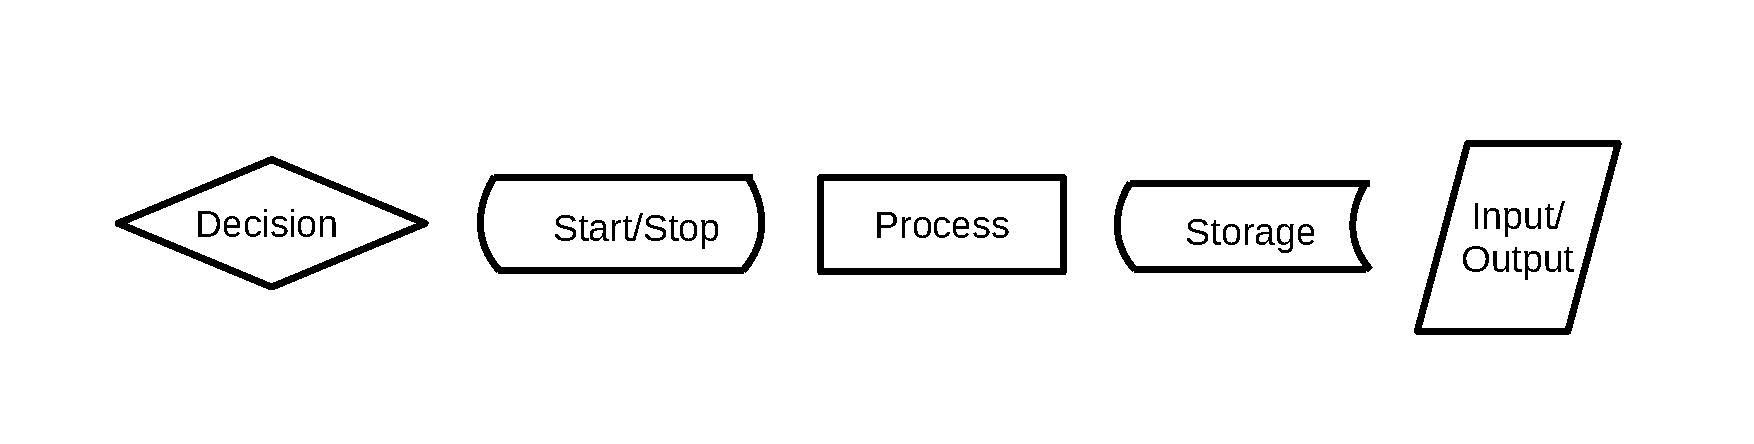
\includegraphics[width=14cm]{FlowchartKey.pdf}\hspace*{\fill}
\end{figure}
\pagebreak

\begin{figure}[H]
\caption{Main Flowchart} \label{fig:LogInFlowchart}
\hfill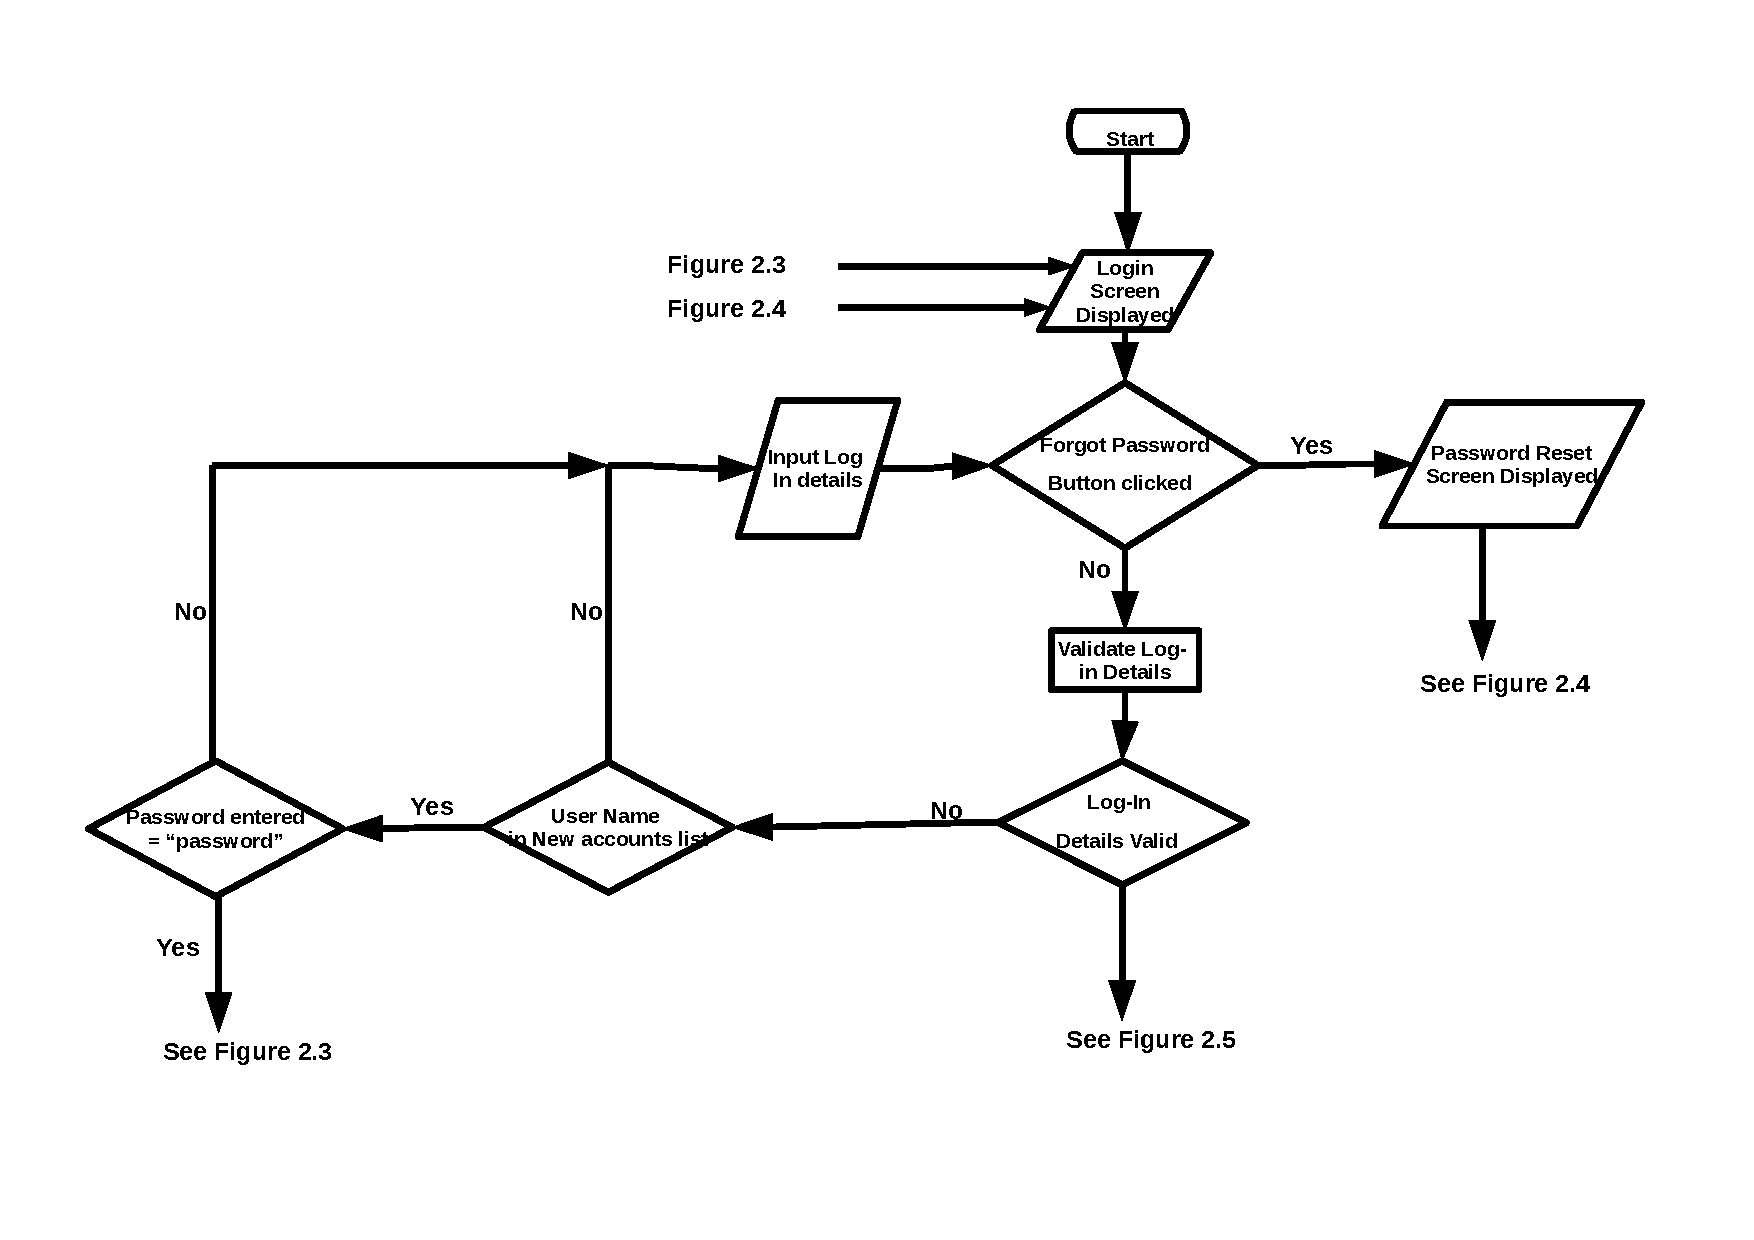
\includegraphics[scale=0.65]{FlowchartMain.pdf}\hspace*{\fill}
\end{figure}
\pagebreak

\begin{figure}[H]
\caption{New Password Flowchart} \label{fig:New Password Flowchart}
\hfill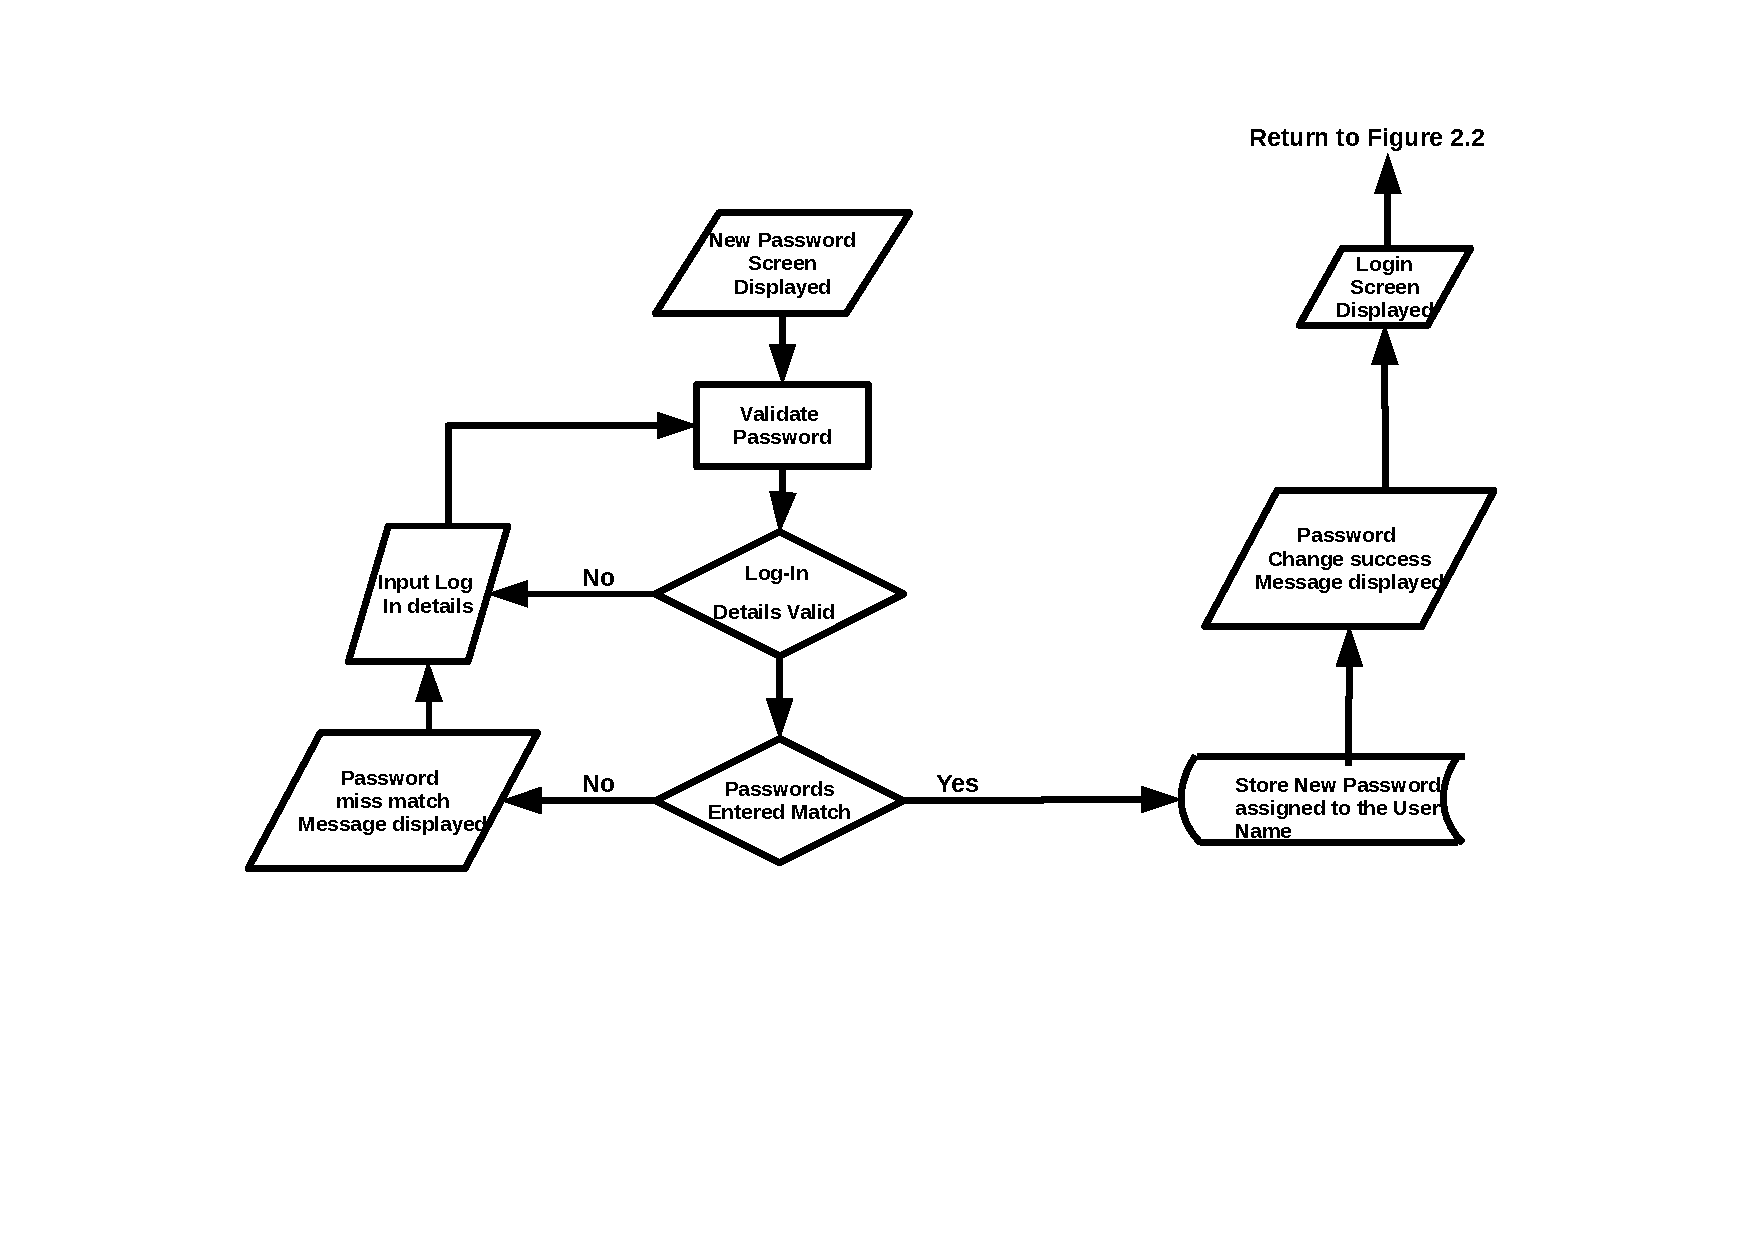
\includegraphics[scale=0.65]{NewPasswordFlowchart.pdf}\hspace*{\fill}
\end{figure}
\pagebreak


\begin{figure}[H]
\caption{Password Reset Flowchart} \label{fig:Password Reset Flowchart}
\hfill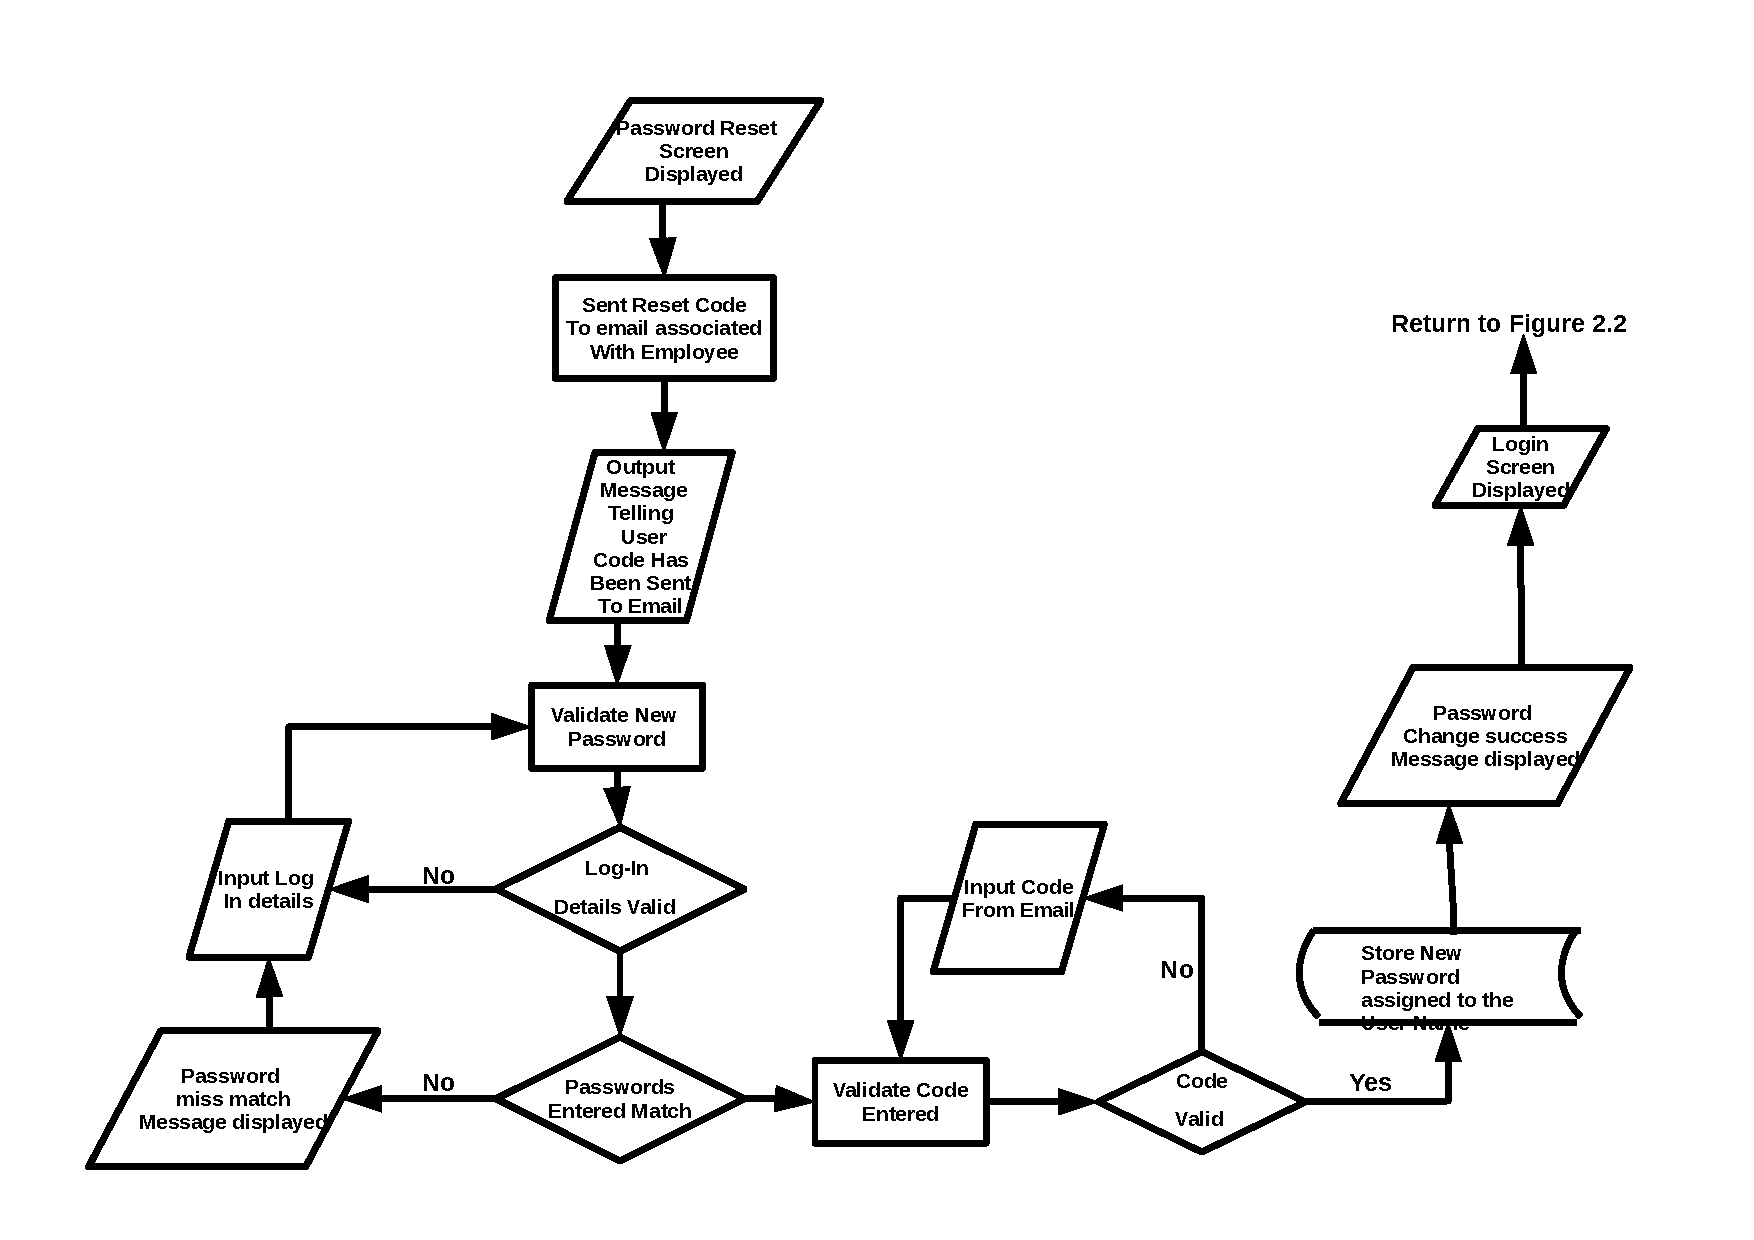
\includegraphics[scale=0.65]{PasswordResetFlowchart.pdf}\hspace*{\fill}
\end{figure}
\pagebreak

\end{landscape}

\begin{figure}[H]
\caption{Options Menu} \label{fig:Options Menu}
\hfill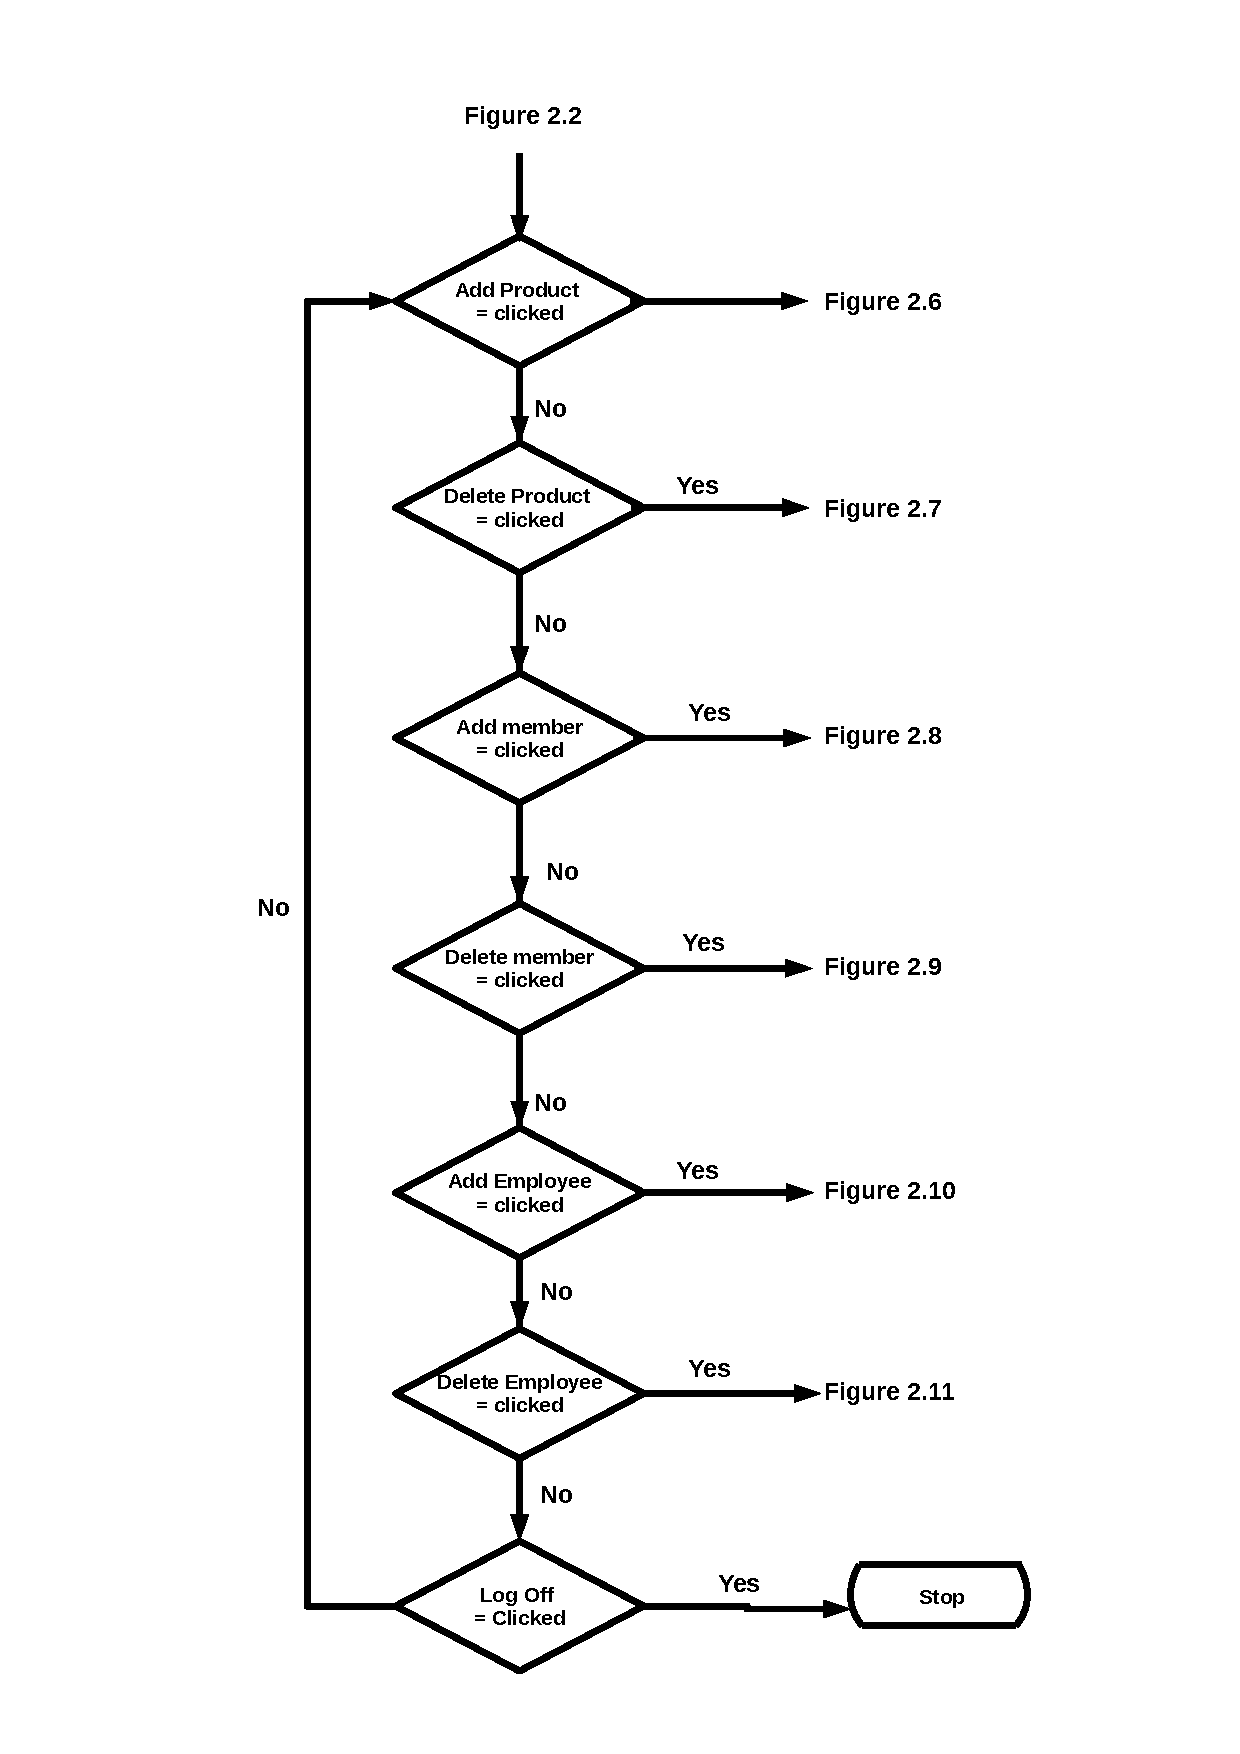
\includegraphics[scale=0.65]{Figure25.pdf}\hspace*{\fill}
\end{figure}
\pagebreak

\begin{landscape}
\begin{figure}[H]
\caption{Add a New Product} \label{fig:Add a New Product}
\hfill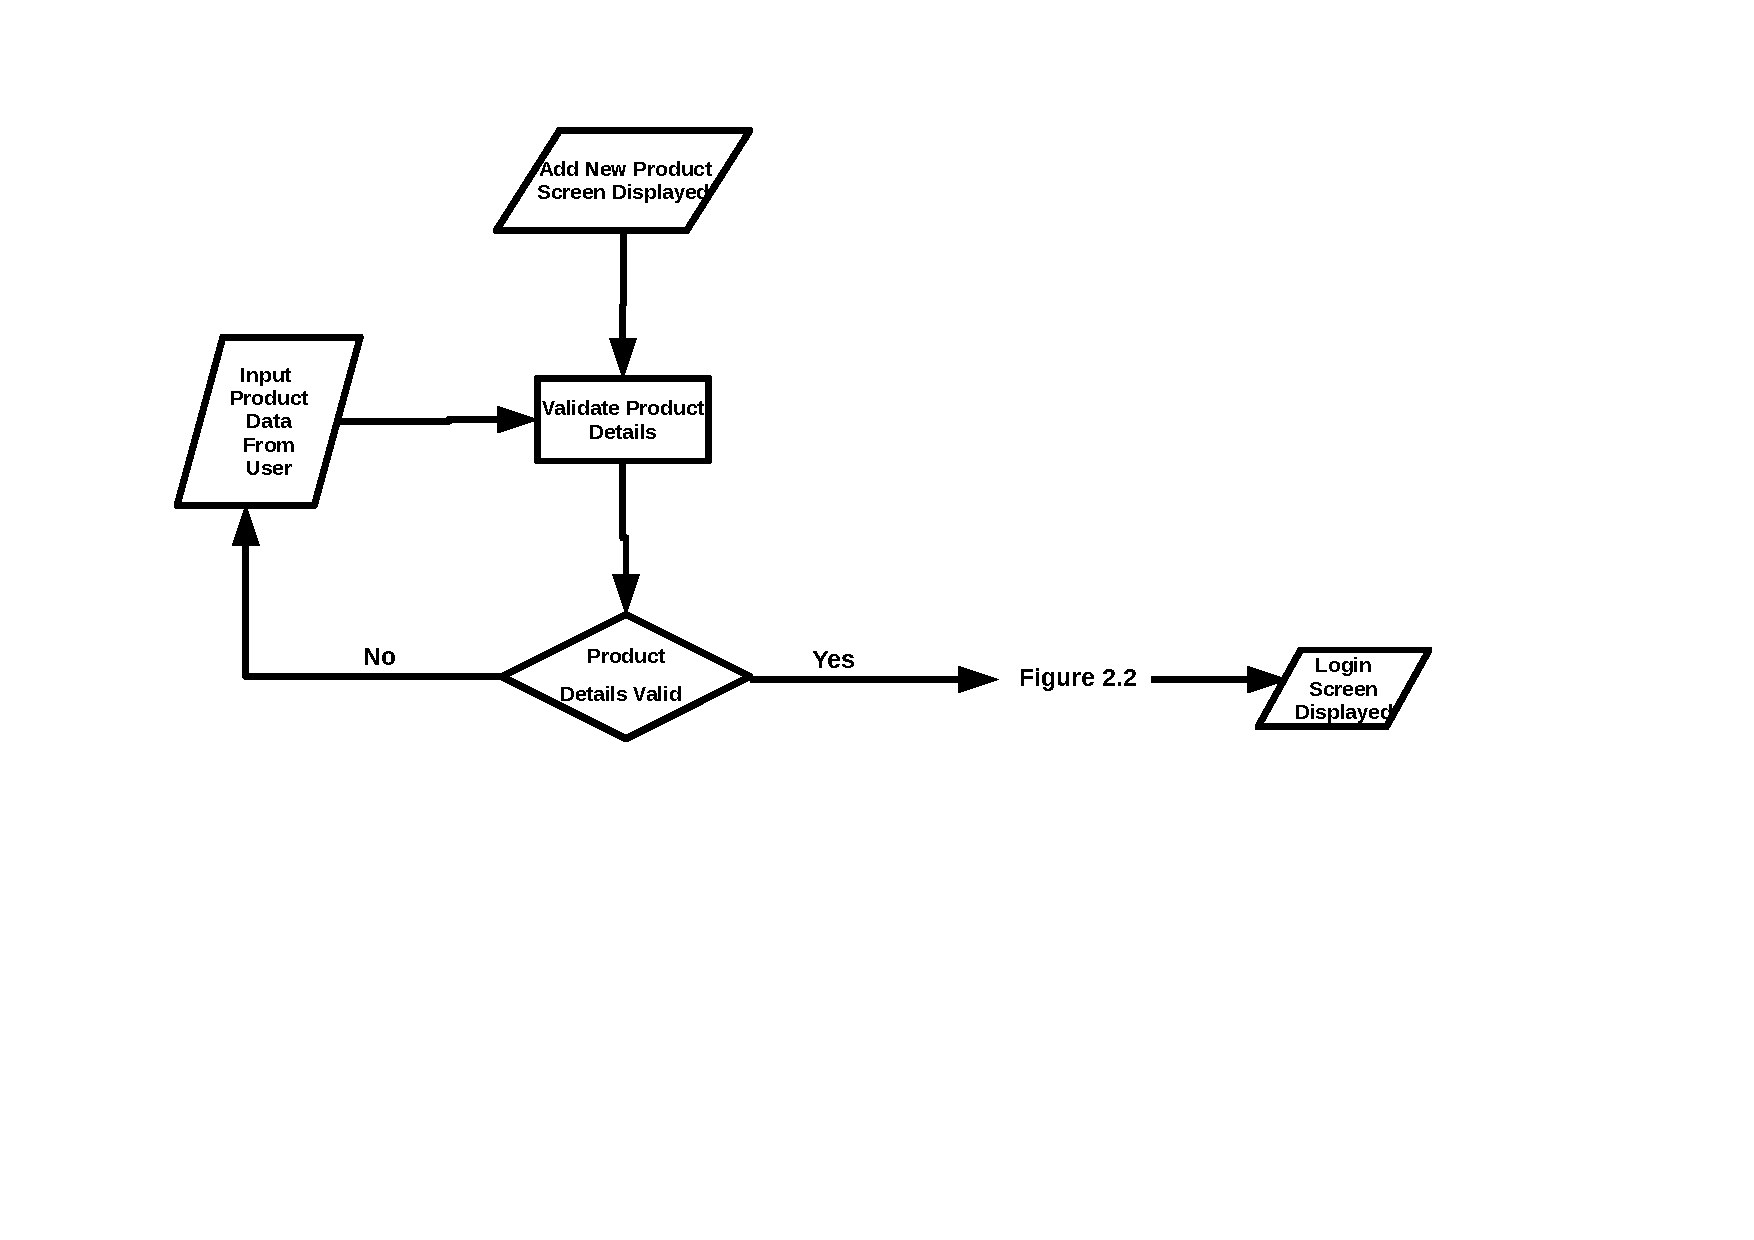
\includegraphics[scale=0.65]{Figure26.pdf}\hspace*{\fill}
\end{figure}
\pagebreak

\begin{figure}[H]
\caption{Delete a Product} \label{fig:Delete a Product}
\hfill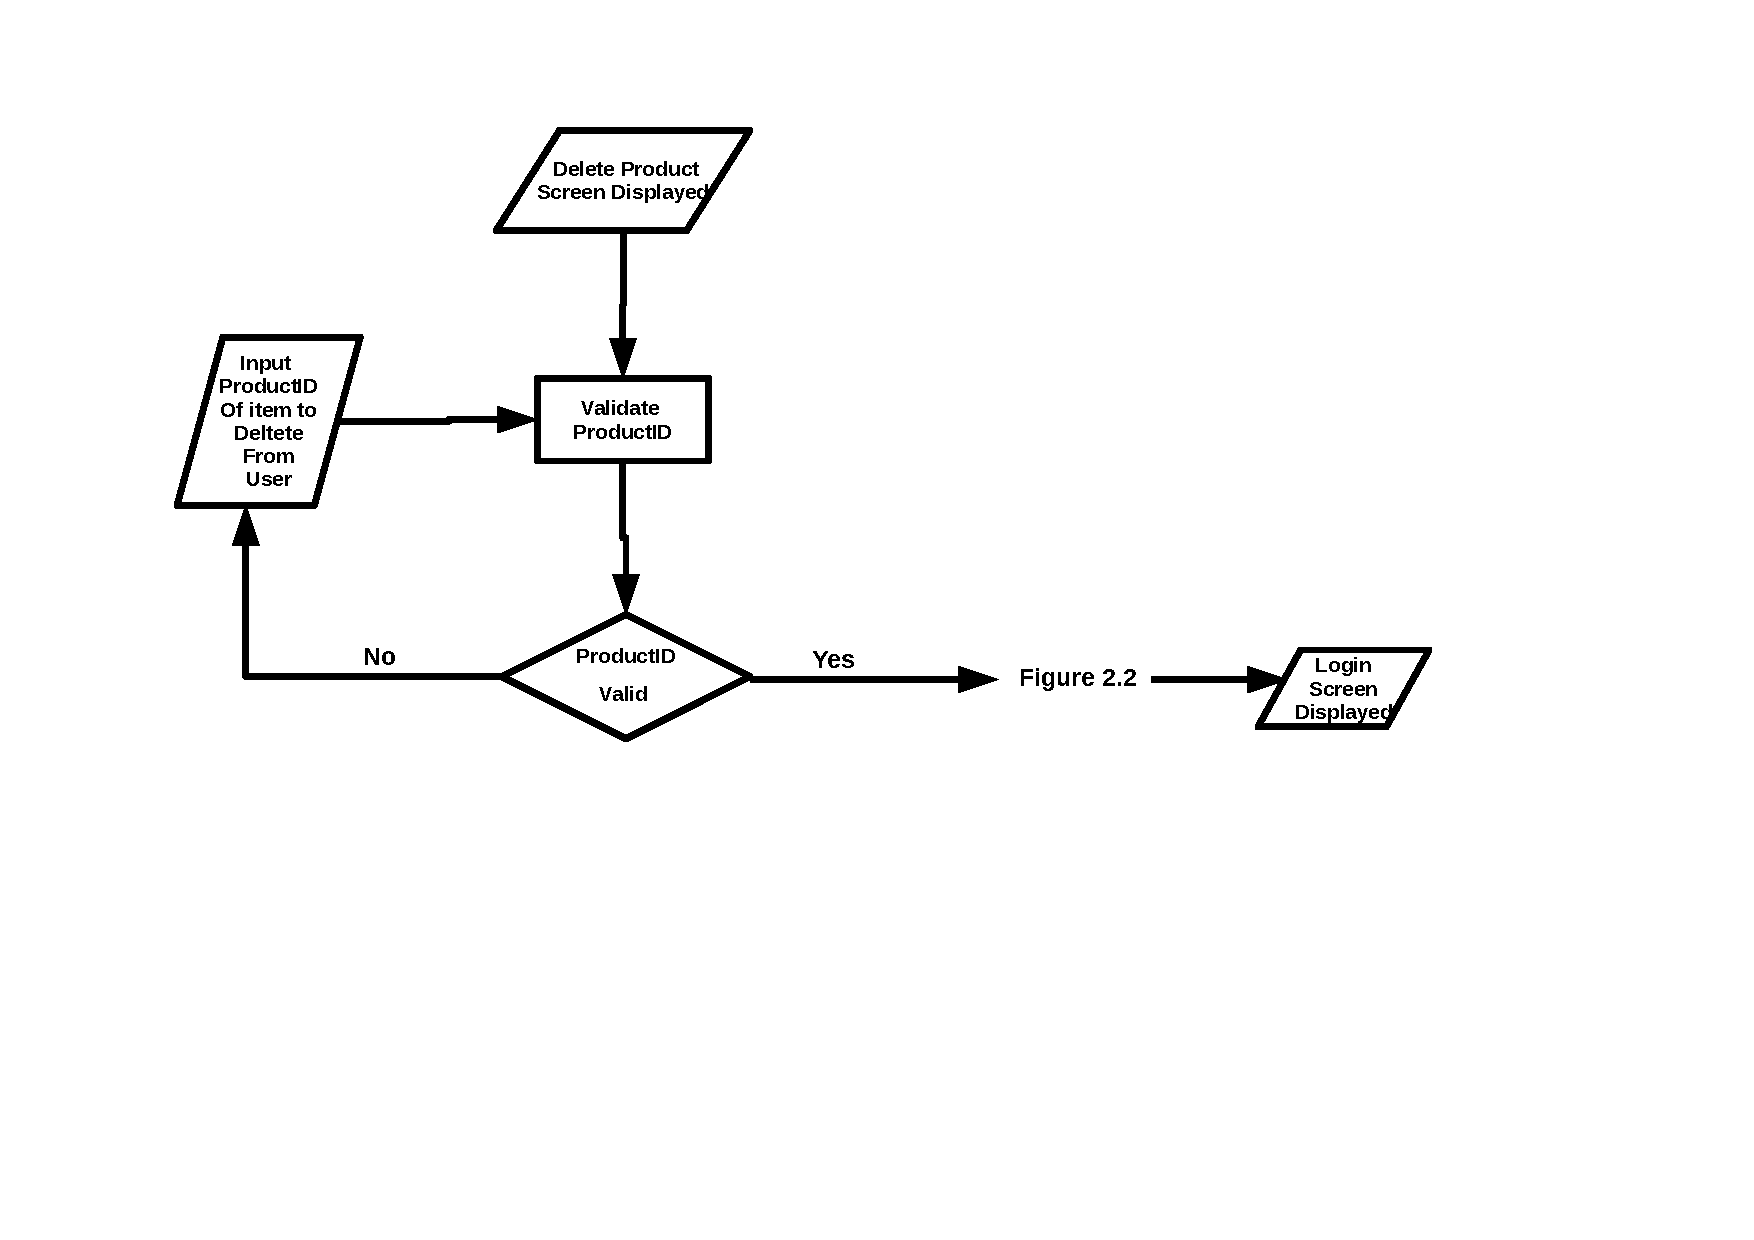
\includegraphics[scale=0.65]{Figure27.pdf}\hspace*{\fill}
\end{figure}
\pagebreak

\begin{figure}[H]
\caption{Add a Member} \label{fig:Add a Member}
\hfill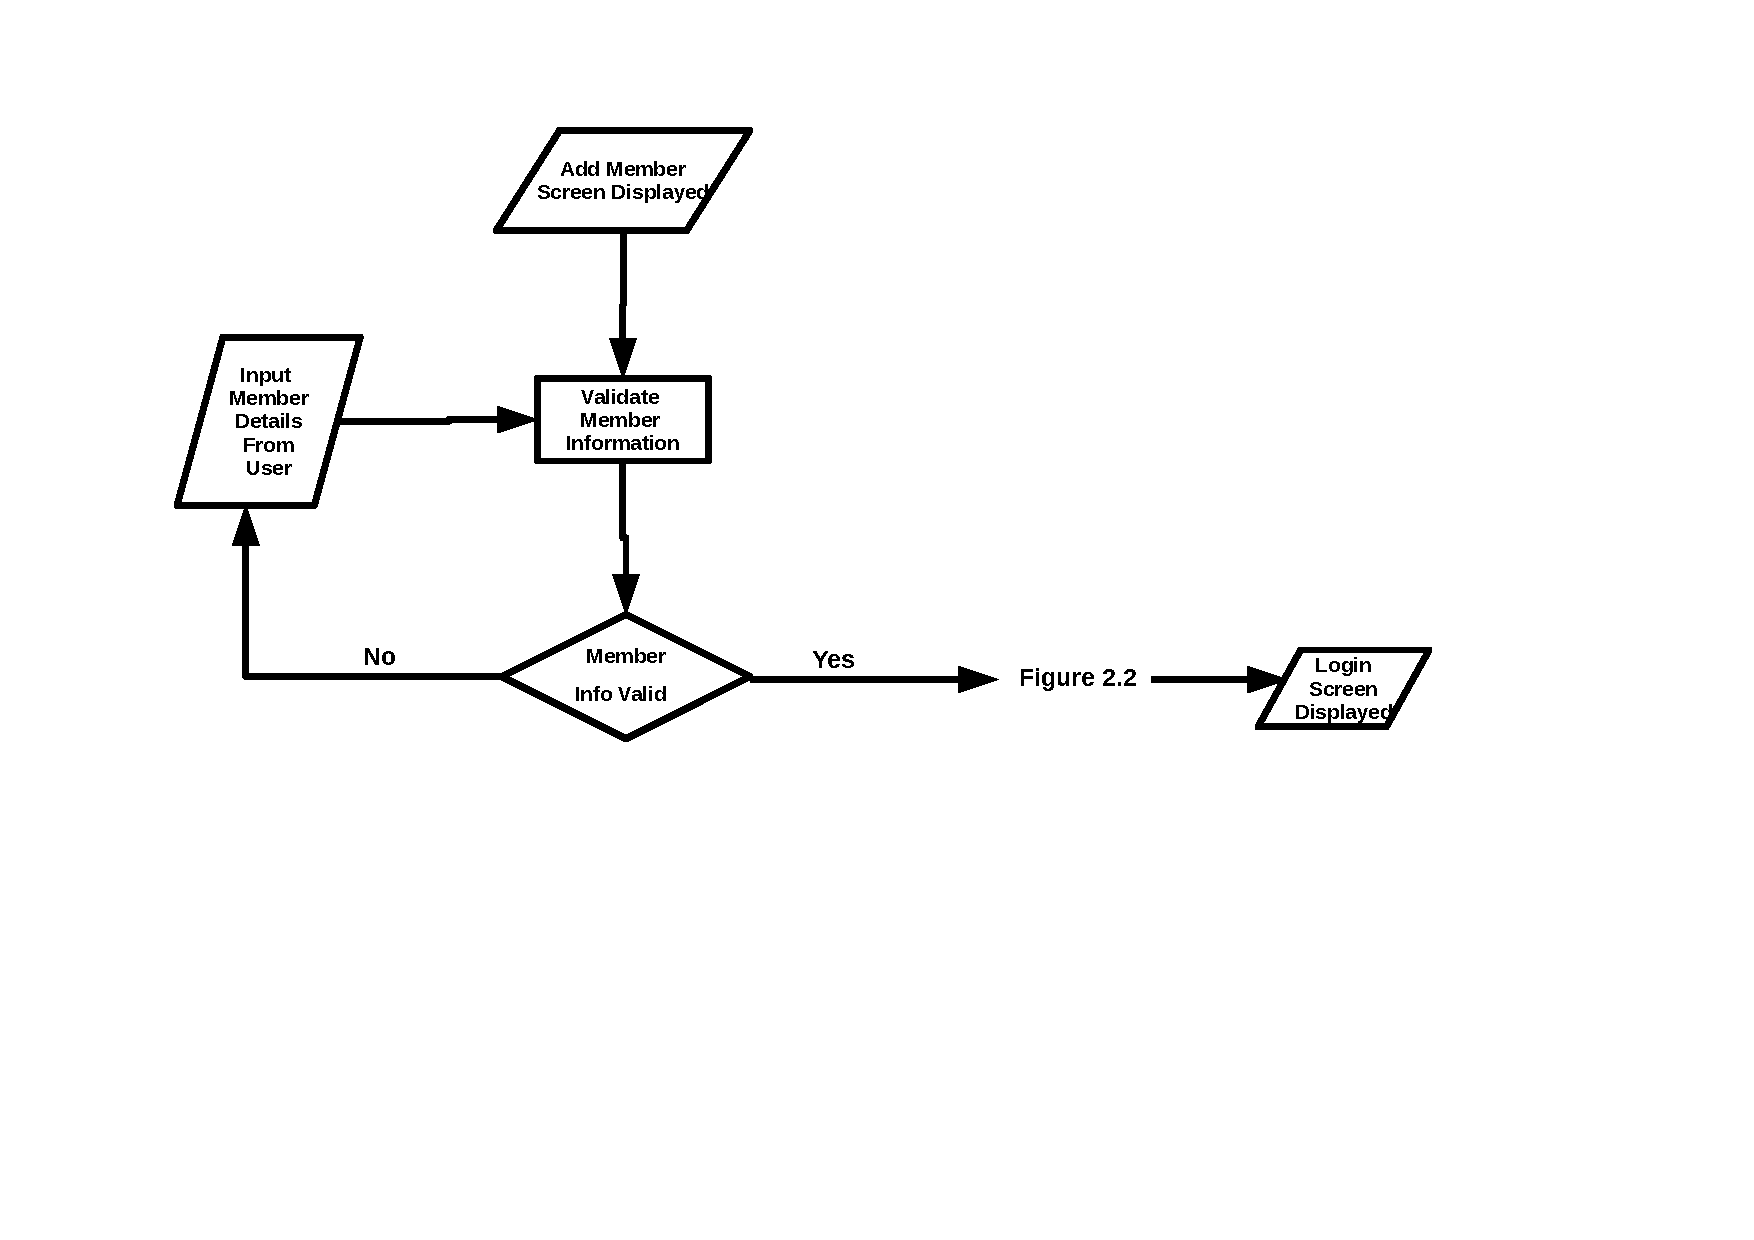
\includegraphics[scale=0.65]{Figure28.pdf}\hspace*{\fill}
\end{figure}
\pagebreak

\begin{figure}[H]
\caption{Delete a Member} \label{fig:Delete a Member}
\hfill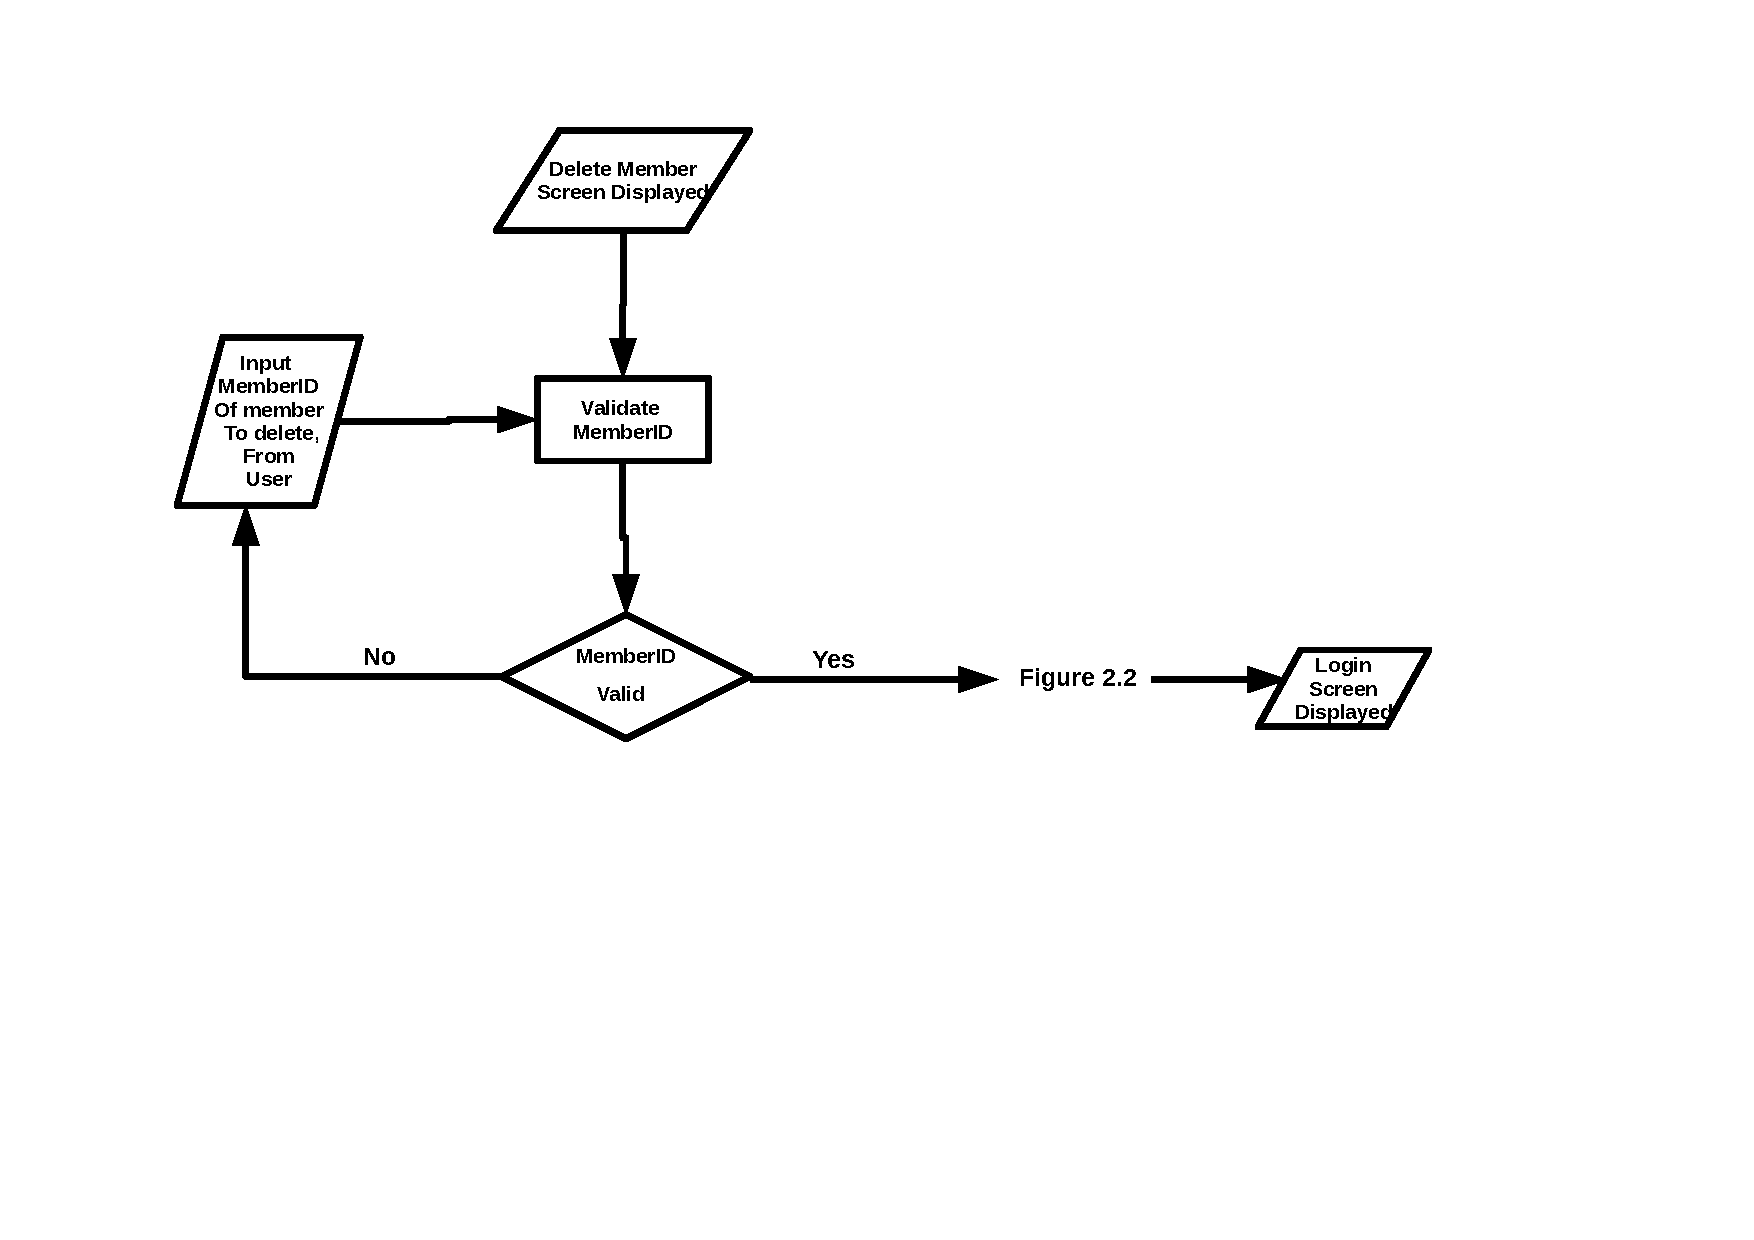
\includegraphics[scale=0.65]{Figure29.pdf}\hspace*{\fill}
\end{figure}
\pagebreak

\begin{figure}[H]
\caption{Add an Employee} \label{fig:Add an Employee}
\hfill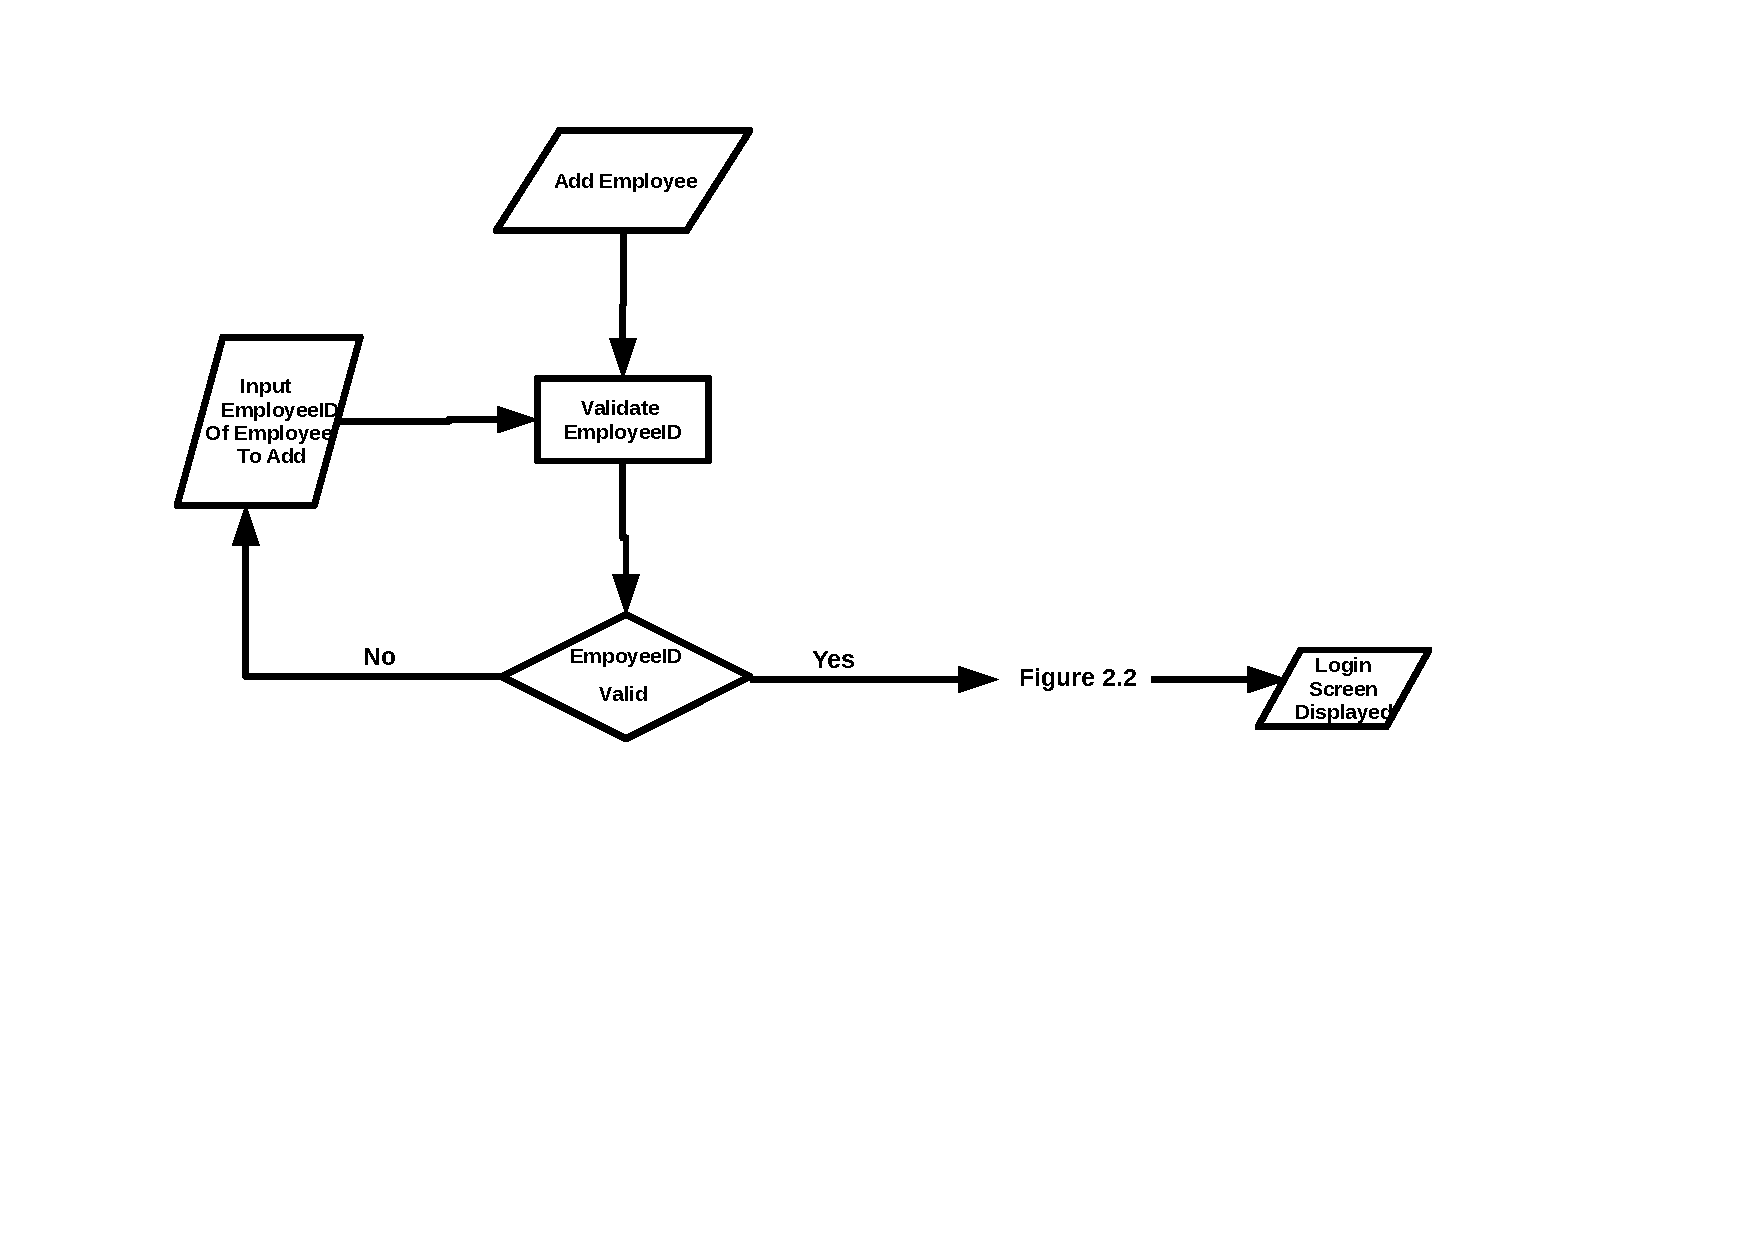
\includegraphics[scale=0.65]{Figure31.pdf}\hspace*{\fill}
\end{figure}
\pagebreak

\begin{figure}[H]
\caption{Delete an Employee} \label{fig:Delete an Employee}
\hfill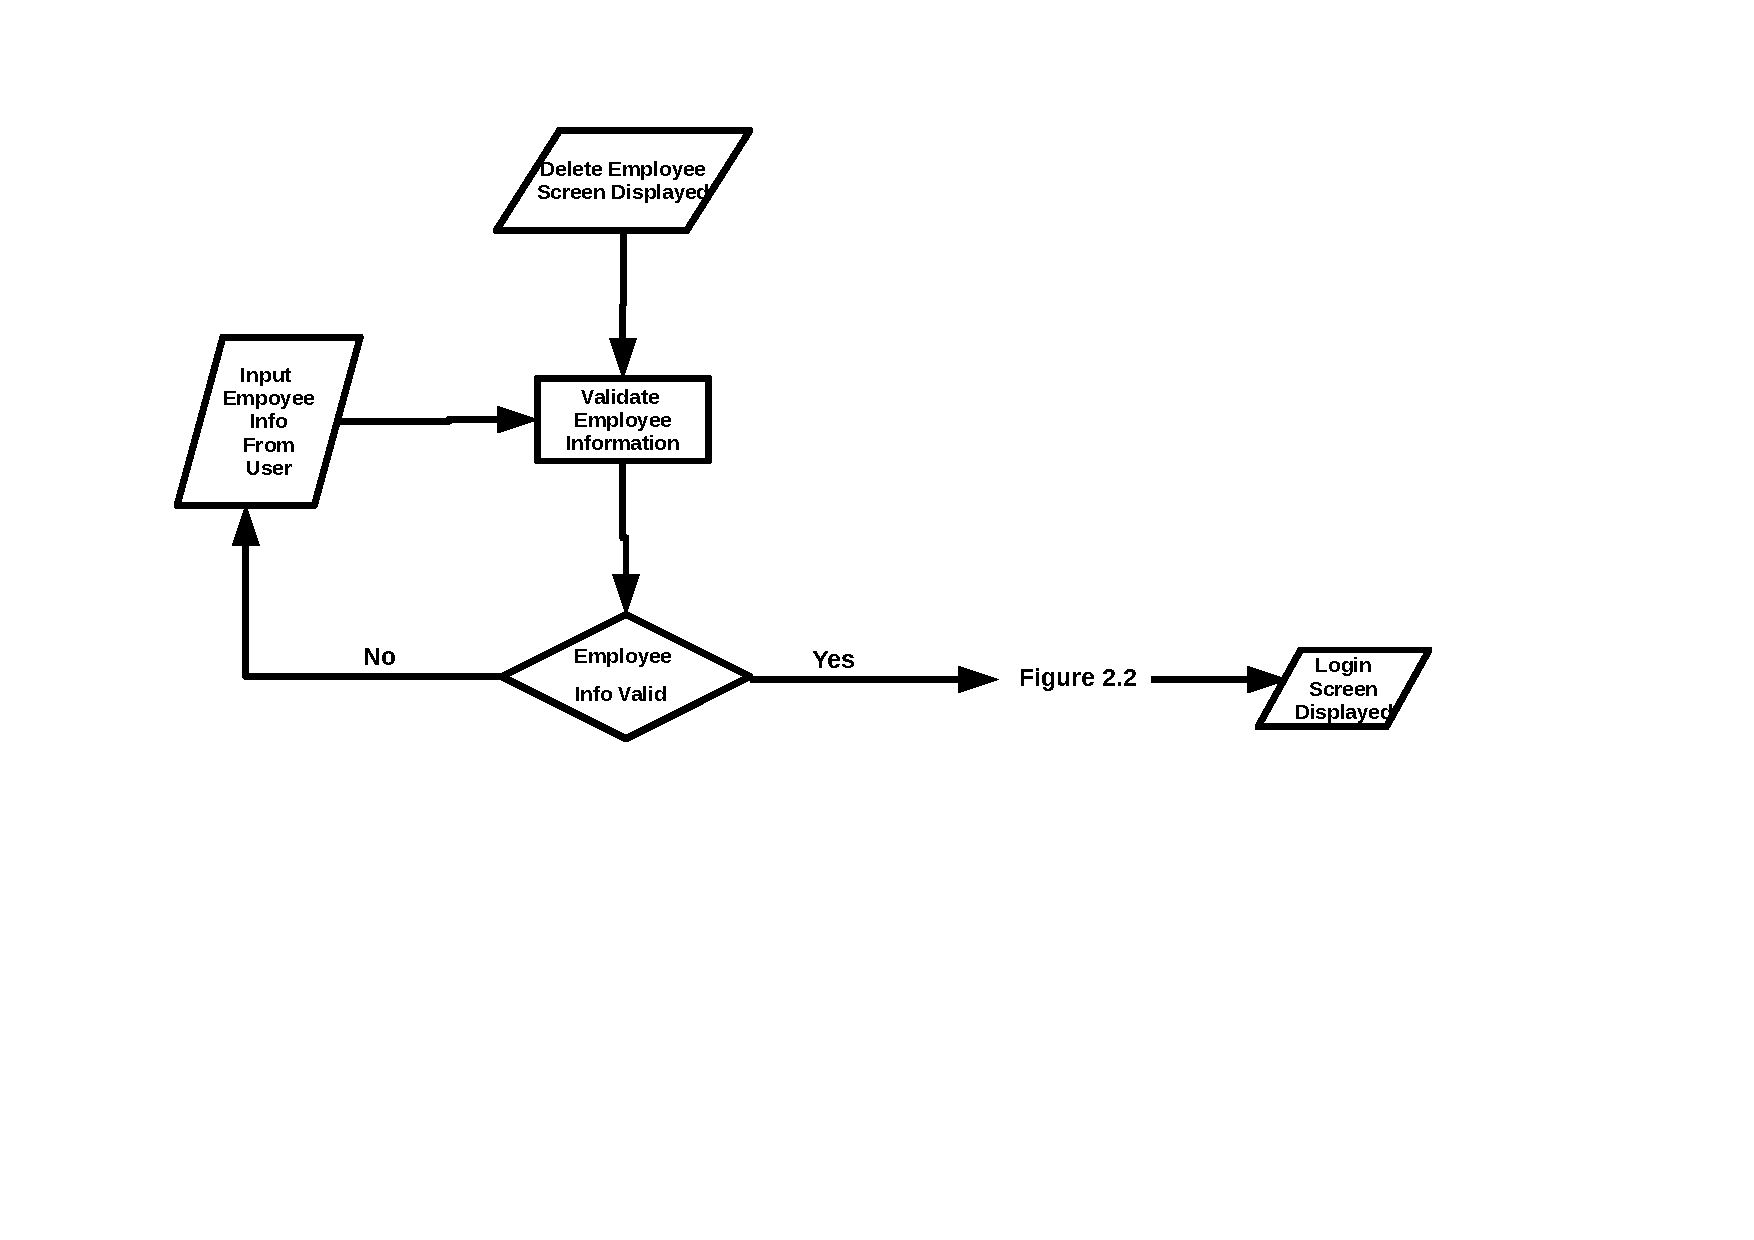
\includegraphics[scale=0.65]{Figure30.pdf}\hspace*{\fill}
\end{figure}
\pagebreak

\end{landscape}
\section{User Interface Designs}


\begin{figure}[H]
\caption{Log In Interface} \label{fig: Log In Interface}
\hfill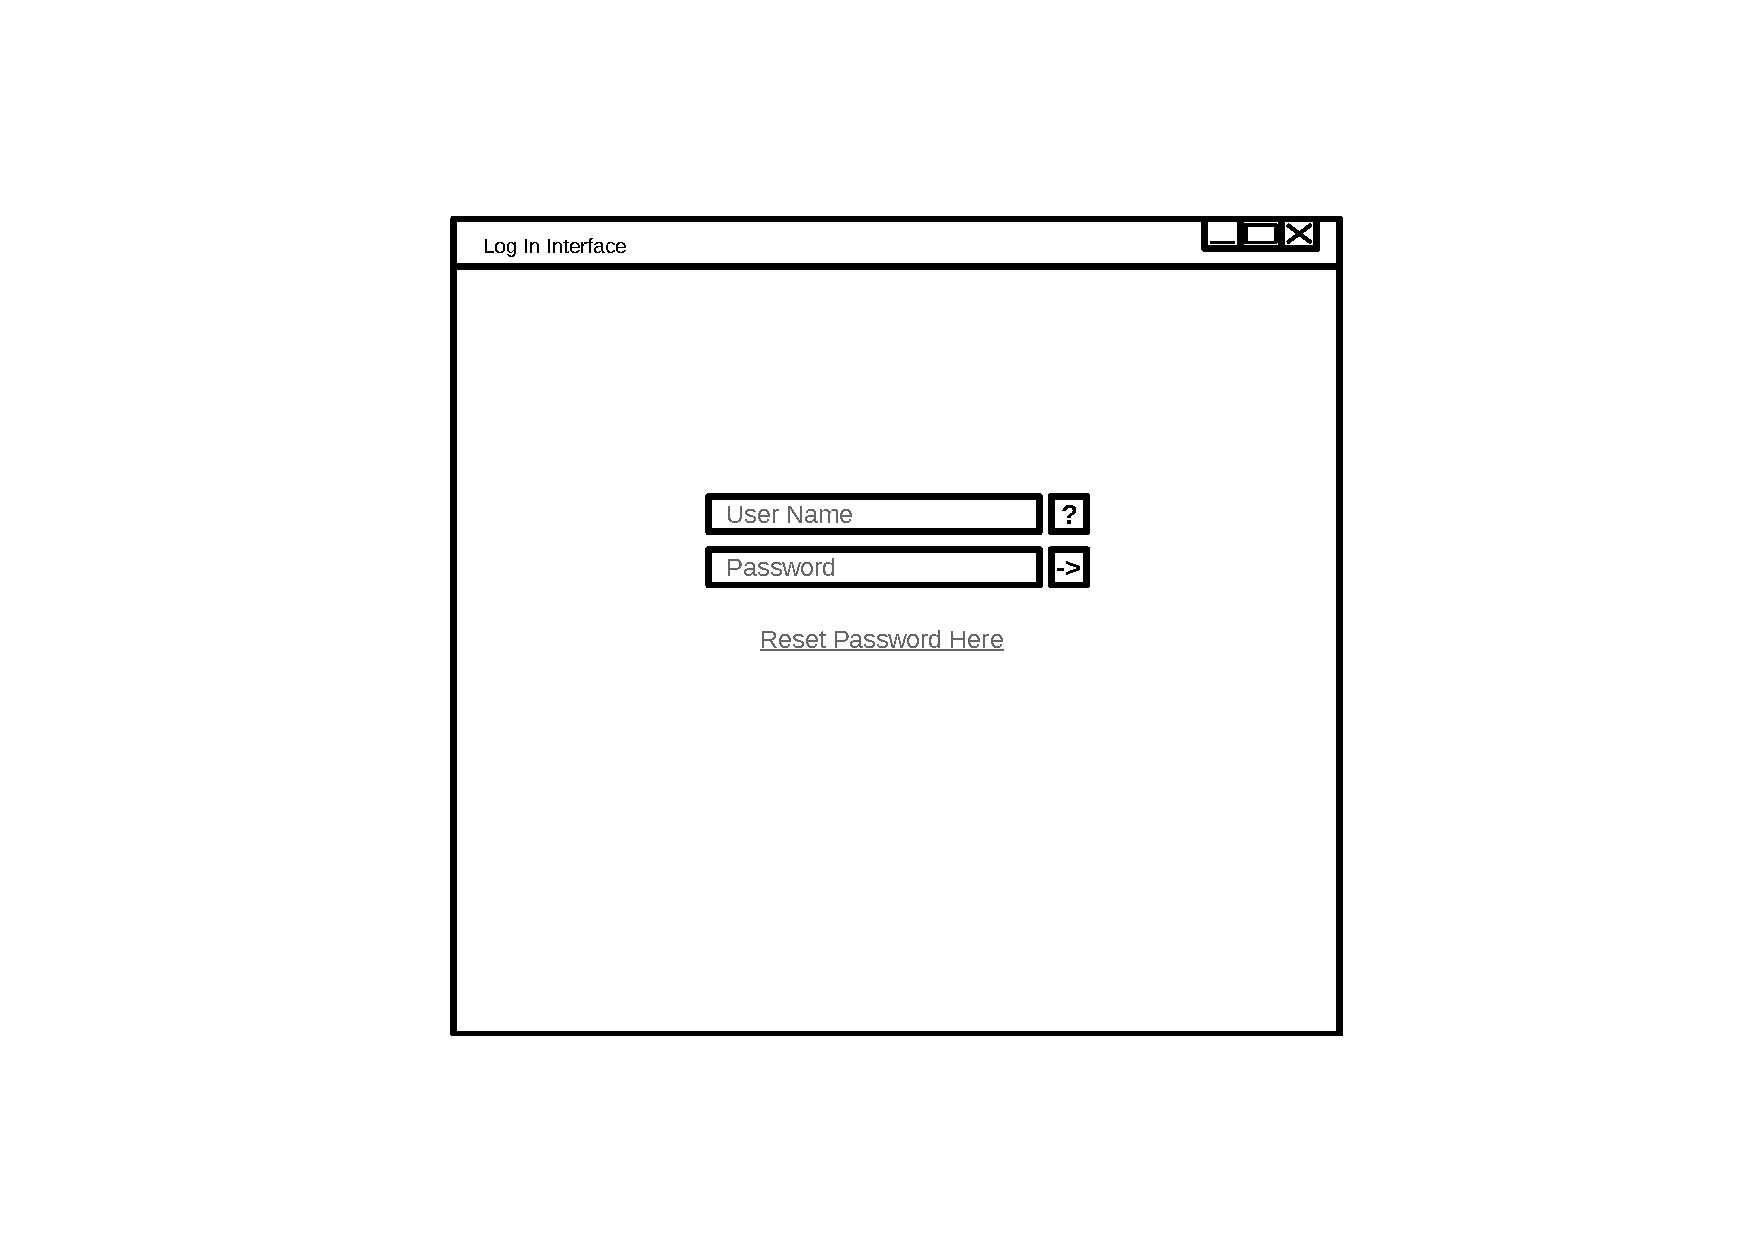
\includegraphics[width = 14cm]{Log-InInterfaceDiagramEdited.pdf}\hspace*{\fill}
\end{figure}


\begin{flushleft}
Looking at Figure 2.12 on Page 51, You can see the Employee Log in interface. The Log In interface contains two fields in which the username and password can be entered and two push buttons, one being the `?' and the other being `->'. The `?' symbol, when clicked, reminds the employee how their username is formed. (First Letter of First Name + Last Name + EmployeeID i.e: MLing03). None of the system is accessible on the log in screen which means that the user MUST log in before they can use the system. This is a security feature as it prevents anyone that does not have a username and password from using the system. The `->' button is simply a click button that checks the employees username and password to see if they are valid. A keyboard shortcut that is commonly assigned to this is `Enter'. \par

If the user clicks on `Reset Password Here' Then the user is directed to a page where they enter a new password to use. A secuirty measure to stop the password being changed by anyone is that the system sends an email to the address assigned to that account, that way, only the employee in which the account is associated with can change the password. \par

\end{flushleft}

\begin{figure}[H]
\caption{Product Search Interface} \label{fig: Product Search Interface}
\hfill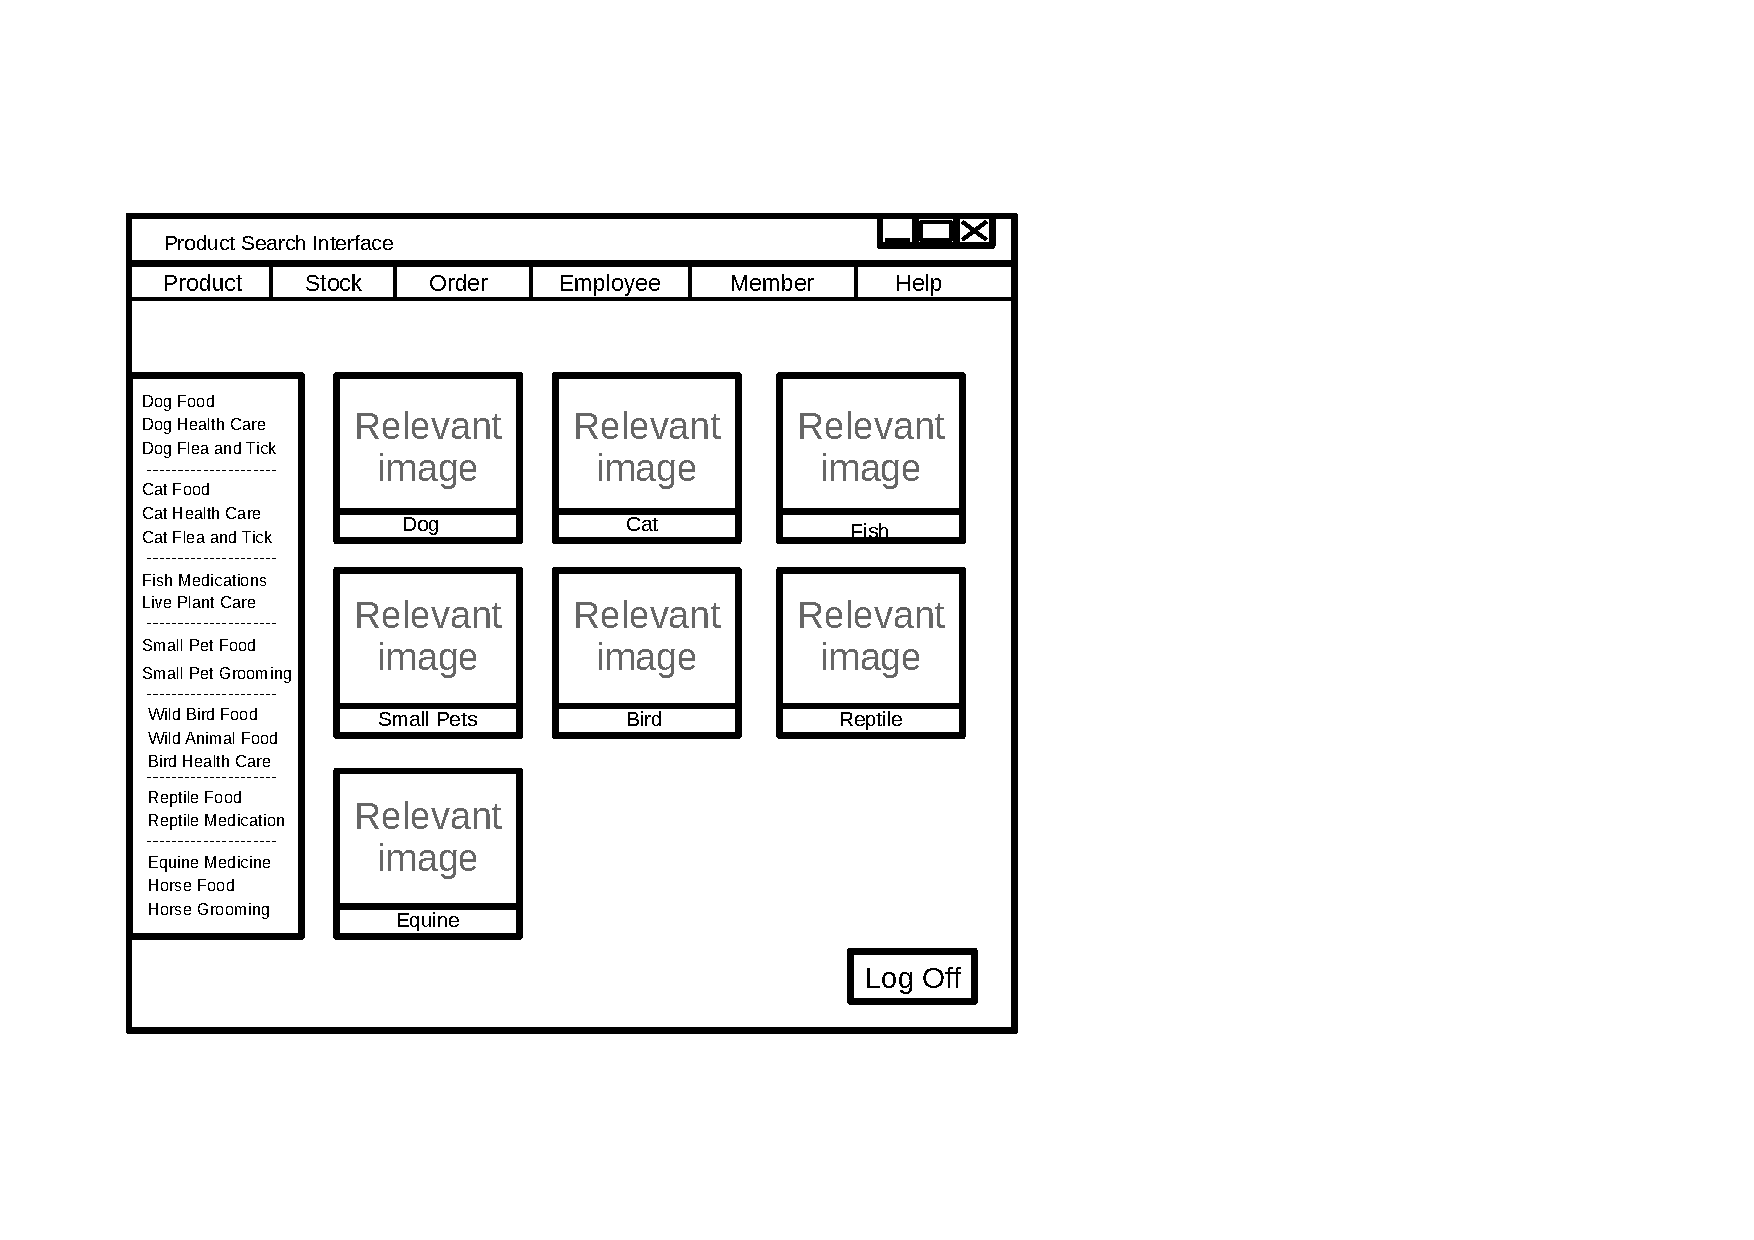
\includegraphics[width = 14cm]{UIDProductSeachInterfaceEdited.pdf}\hspace*{\fill}
\end{figure}

Figure 2.13 is the Product Search Interface, This will also act as the main menu as this will be the most commonly used interface. Once the user has logged in, The six tabs are always displayed at the top of the application, no matter what interface they are on (other than the log in interface). \par

The product Search interface is used when the user wants to find a specific product. This can be done one of three ways. If the user knows the name of the product they are looking for, they can simply use the search bar which is described later in the User Interface Design Section. Alternatively the user can Go to the Product Search interface and click on the large buttons that are made up of an Animal and a picture of that animal, by clicking on that button, The user will then have to click on the category in which the product falls under(i.e food / health care) The user will then be given a table of all the products that fall under that category. The user will be able to sort the products to find the product they are looking for. \par

However, going from a product from one category to a product from another category may be quite confusing going back and forth between categories, pressing multiple buttons. Therefore a list down the left hand side of the page has Each Category Sorted into each Animal. The user can then jsut simply click on the category and they will be taken straight to the products. This method will allow the user to find products faster by reducing time selecting categories. \par

When The user has finished using the system, they can return to the Product Search interface and click the `Log Off' button. This will log the user out and will require an employee to enter their log in details before the system can be accessed again. if the application is closed using the close button in the top right hand corner, without the user logging out, the user will automatically be logged out. However if the user clicks the close button, a warning message will be displayed to confirm they want to close the application. This prevents the application from closing when the user accidentally clicks the close button. \par

\begin{figure}[H]
\caption{Right Click Options For MenuBars} \label{fig:Right Click Options For MenuBars}
\hfill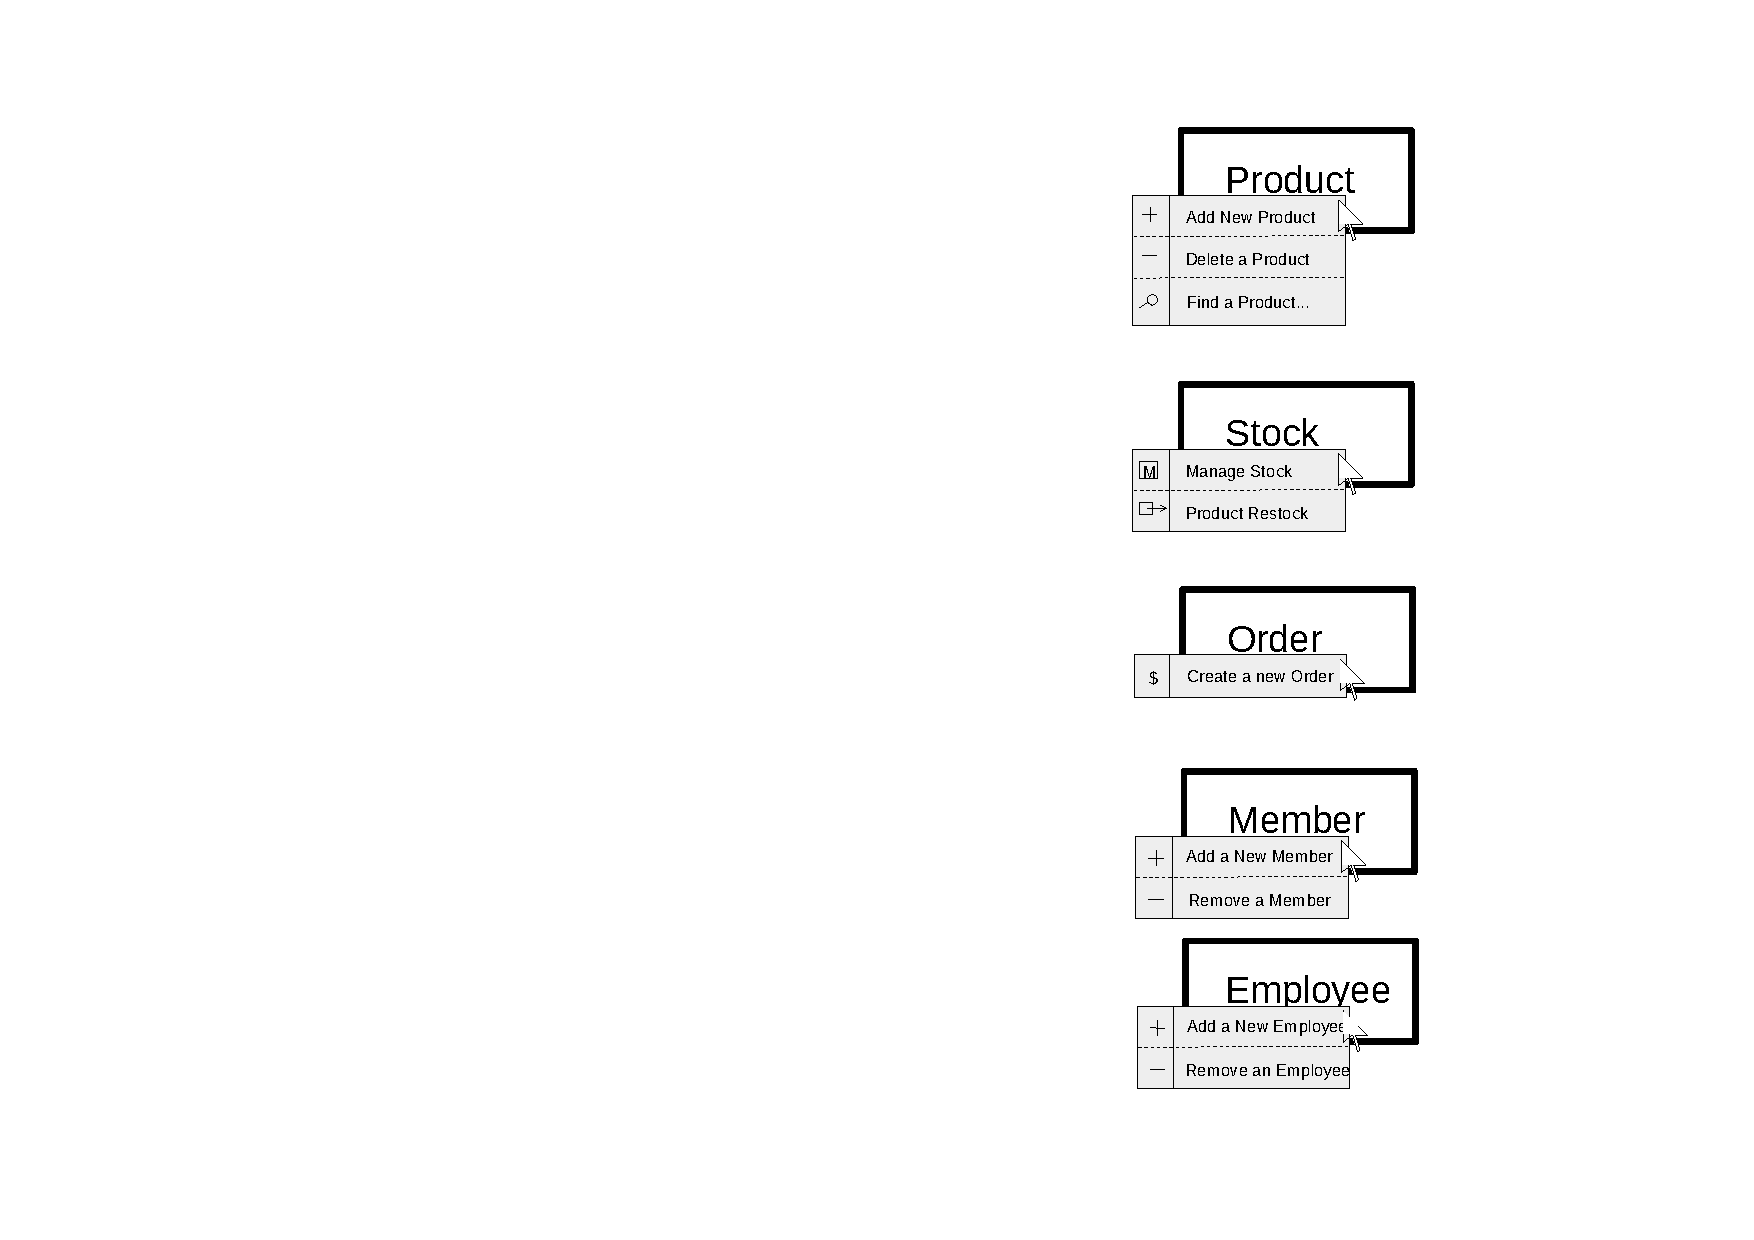
\includegraphics[width = 6cm]{UIDProductSeachInterfaceMenus.pdf}\hspace*{\fill}
\end{figure}

Looking at Figure 2.14 and referring back to Figure 2.13, we can see the options that appear when each tab is clicked. Each option has a symbol next to it to easily identify the option the user wants. When add new product is selected, the user is taken to the add new product interface. Deleting a Product / Member / Employee Account will ask for the ID for the item they user wants to delete, then remove all the data relating to the ID from the sytem. The Manage Stock, Add New Member and Add new Employee buttons will take the user to the corresponding interface. To navigate between the pages, the user can will use the menu to select the page they want to go to. For example, if the user is on the Add new Product screen and wants to go to the Add new Member, They go to The Member Menu then select Add new Member. Their current page will then change to the new page they selected. An example of this is shown below:\par

\begin{figure}[H]
\caption{Right Click Options For MenuBars} \label{fig:Right Click Options For MenuBars}
\hfill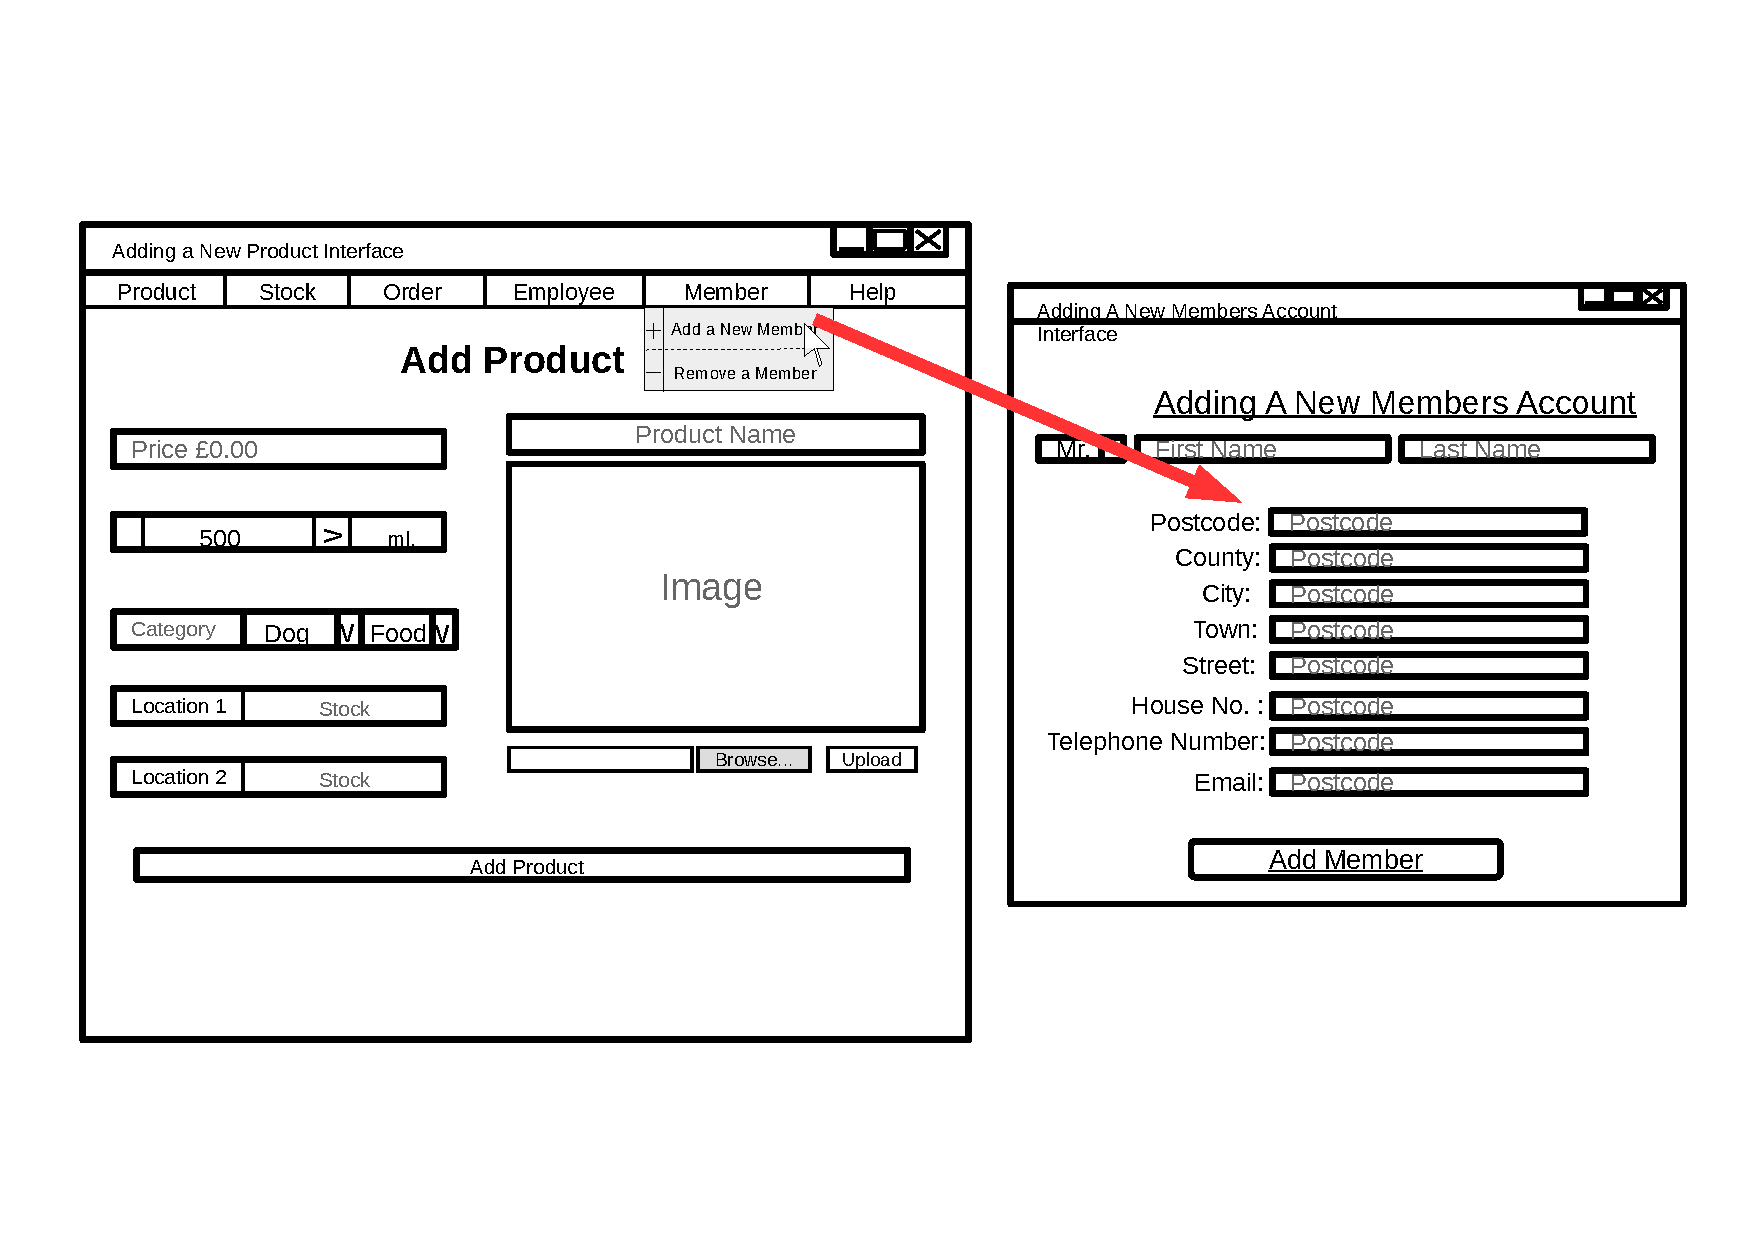
\includegraphics[width = 6cm]{ChangingInterfaceDiagram.pdf}\hspace*{\fill}
\end{figure}

\pagebreak

\begin{figure}[H]
\caption{Adding a New Product} \label{fig:Adding a New Product Interface}
\hfill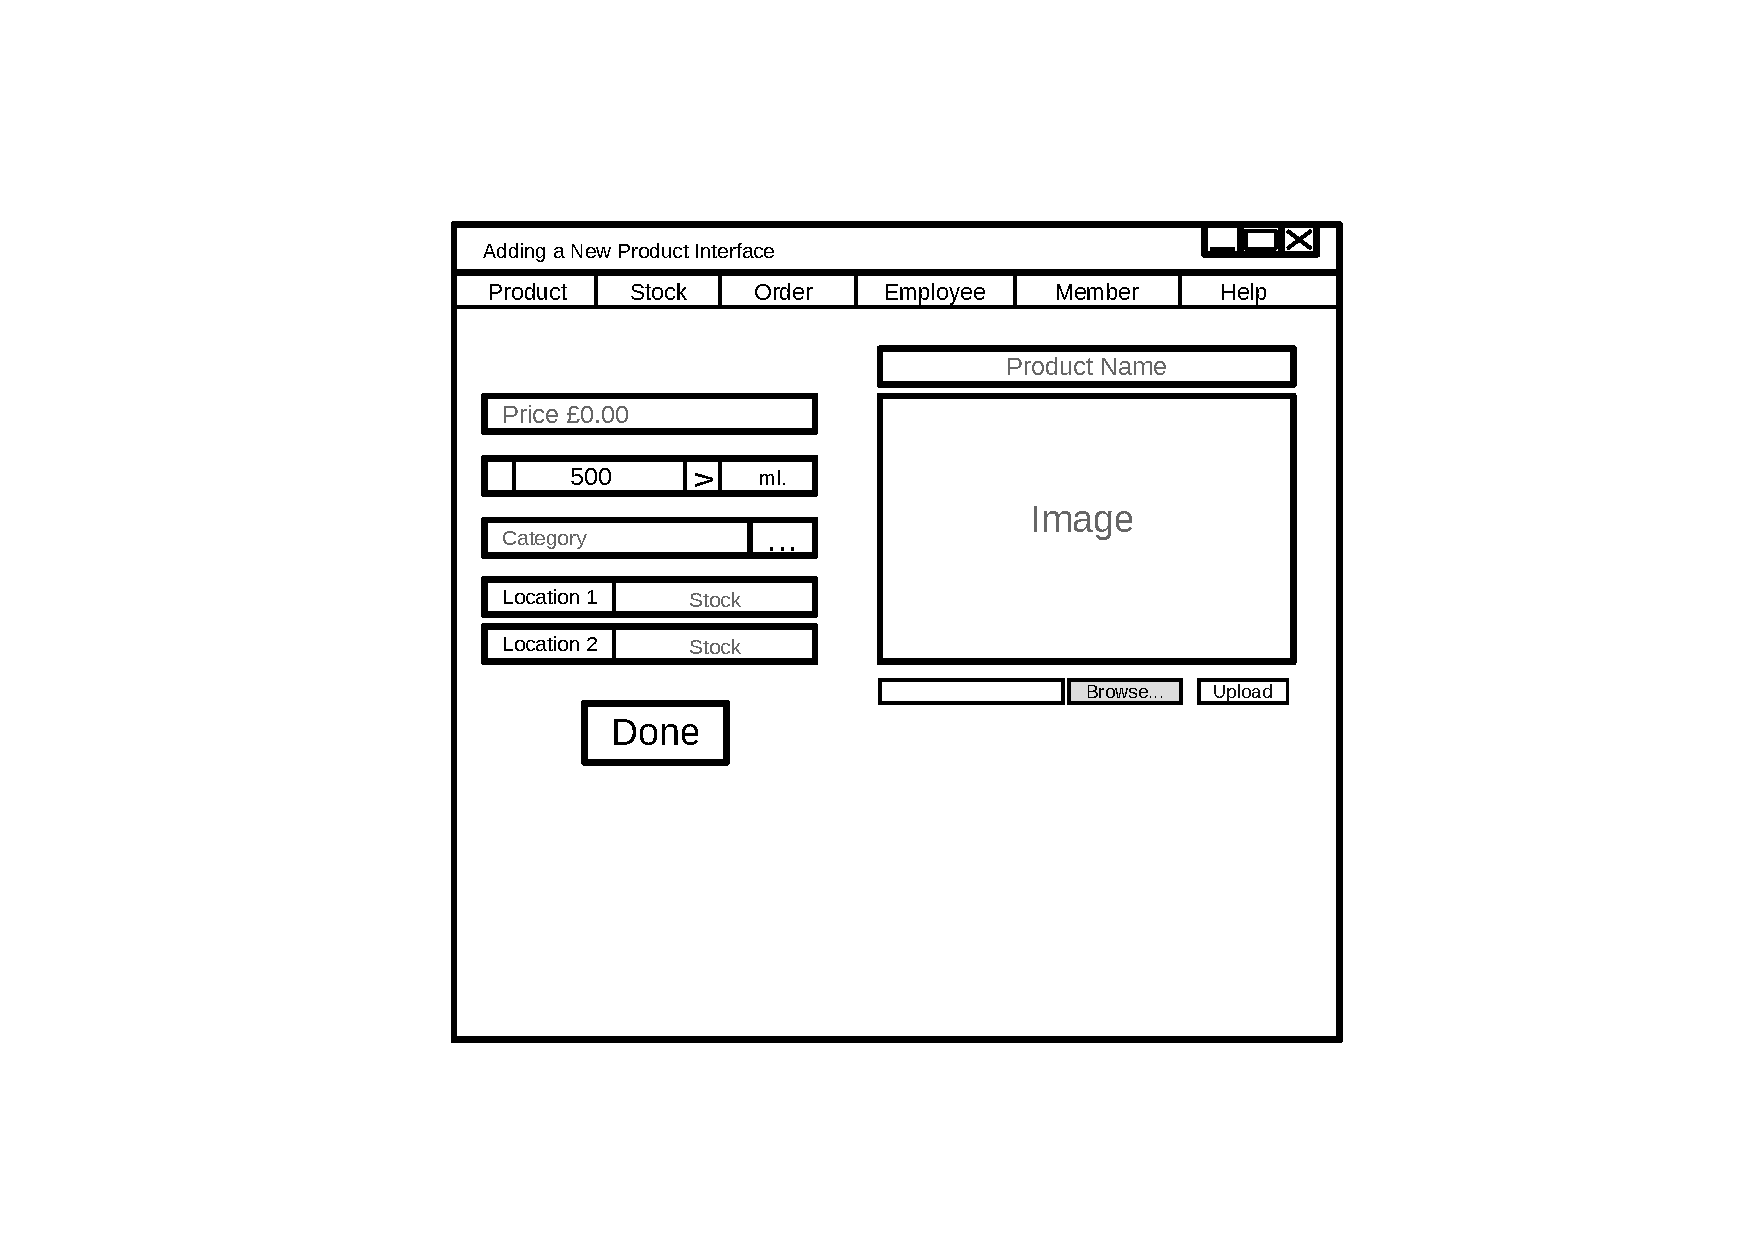
\includegraphics[width = 14cm]{UIDAddingAProductEdited.pdf}\hspace*{\fill}
\end{figure}

Figure 2.15, is the Adding a New Product Interface. Here there is a field in which the user can enter the Product name and the price. To upload an image, the user much click the browse button which will open a window in which the user can select the image file of their choice. once the user has selected the file they must click upload. Once clicked, the upload button will crop the imagine to fit the image area and will display the image to the user, so they can change the image if need be before the product is added to the system. \par

The user has the option to enter any value between 1-1000 in the field that is currently `500' in the diagram.  This field is to specify the specific size of an item. For example there might be two types of the same dog food, one 500 grams one 750 grams. The value is then followed by a drop down menu. \par


\begin{figure}[H]
\caption{Drop Down Menu} \label{fig:Drop Down Menu}
\hfill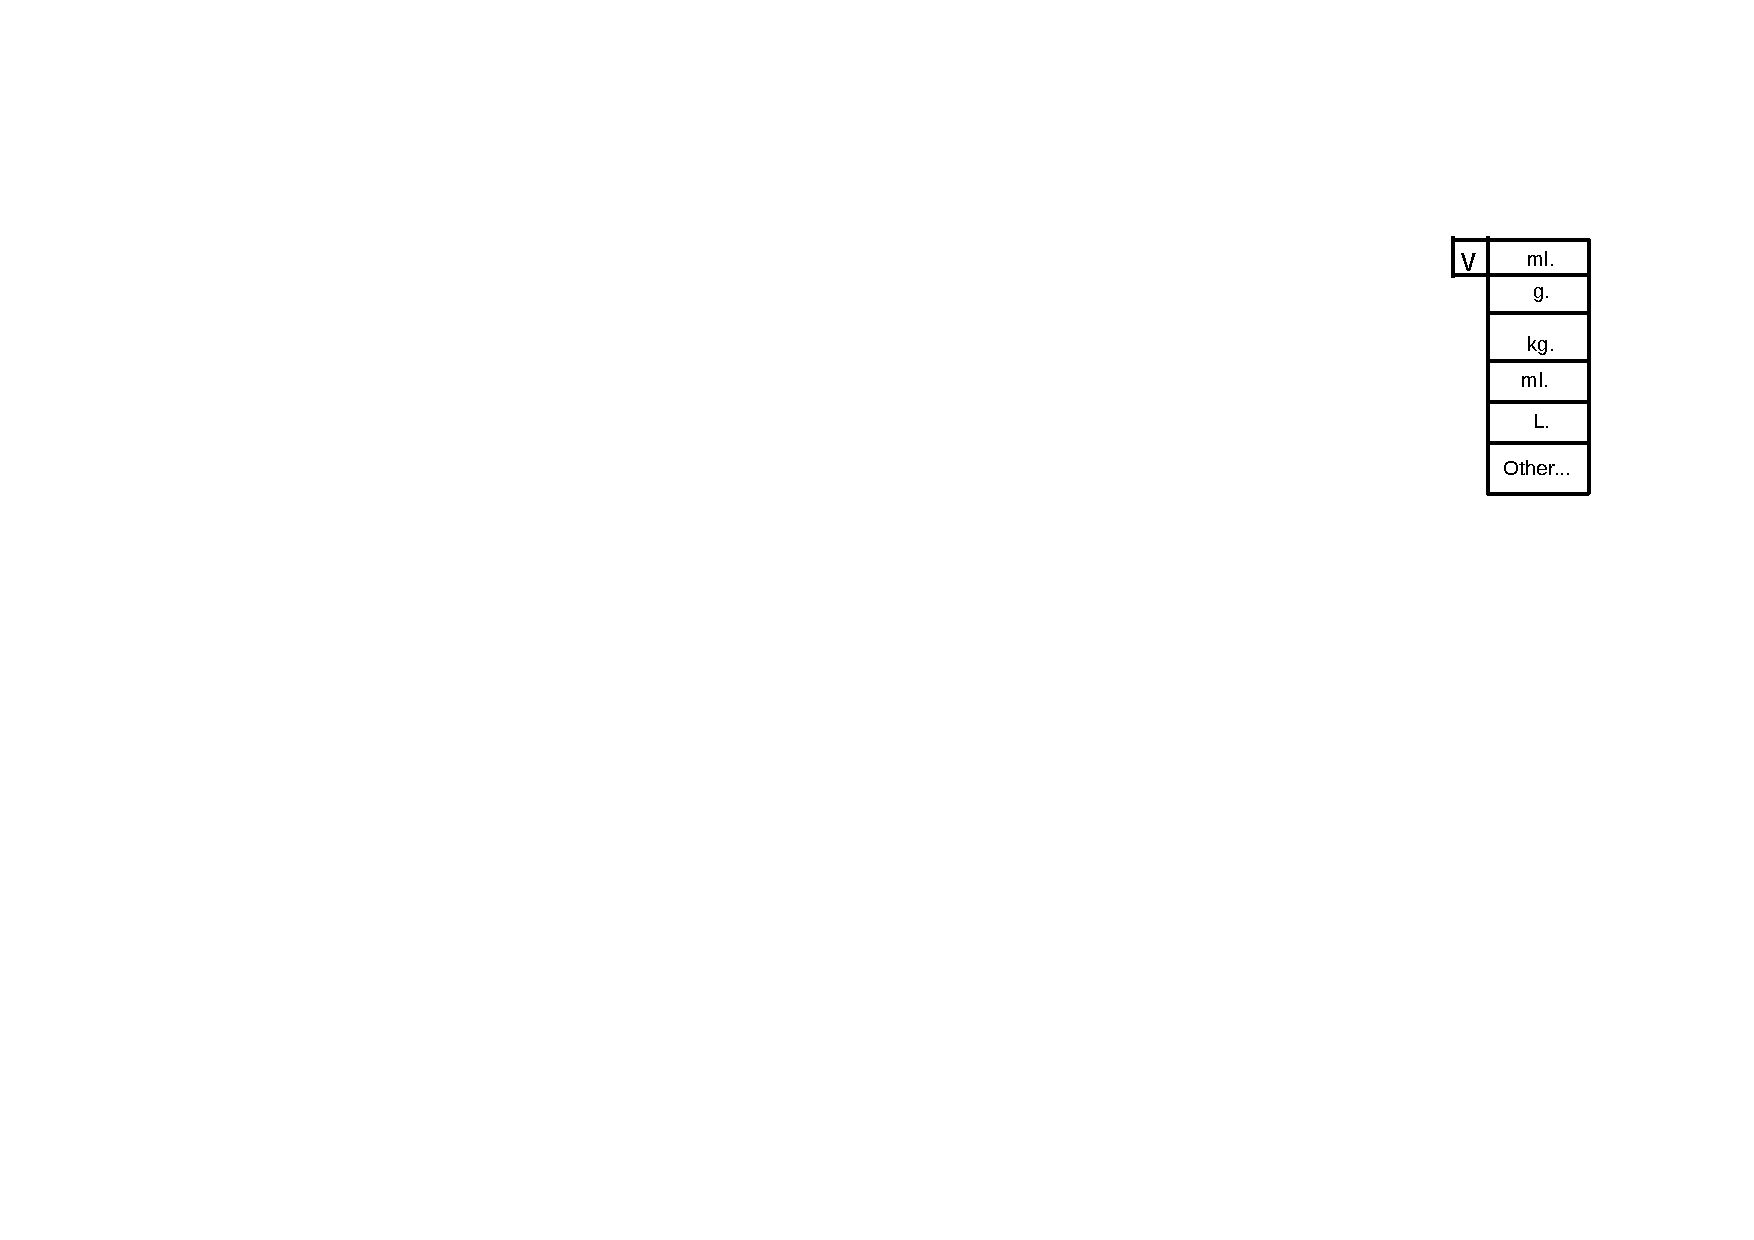
\includegraphics[width = 4cm]{DropDownMenuAddingProduct.pdf}\hspace*{\fill}
\end{figure}

This drop down menu contains the four most common quantities but incase the product does do not fall under any of those quantities, the user can click on the other option, which will allow the user to then enter a custom quantity. \par

The user then has to enter the stock of the product in each location. Once the user has completed all the fields, they can review the information and then click the `Done' button. The `Done' button will then create a New product, with the attributes entered by the user. \par

\begin{figure}[H]
\caption{Adding a New Employee} \label{fig:Adding a New Employee Interface}
\hfill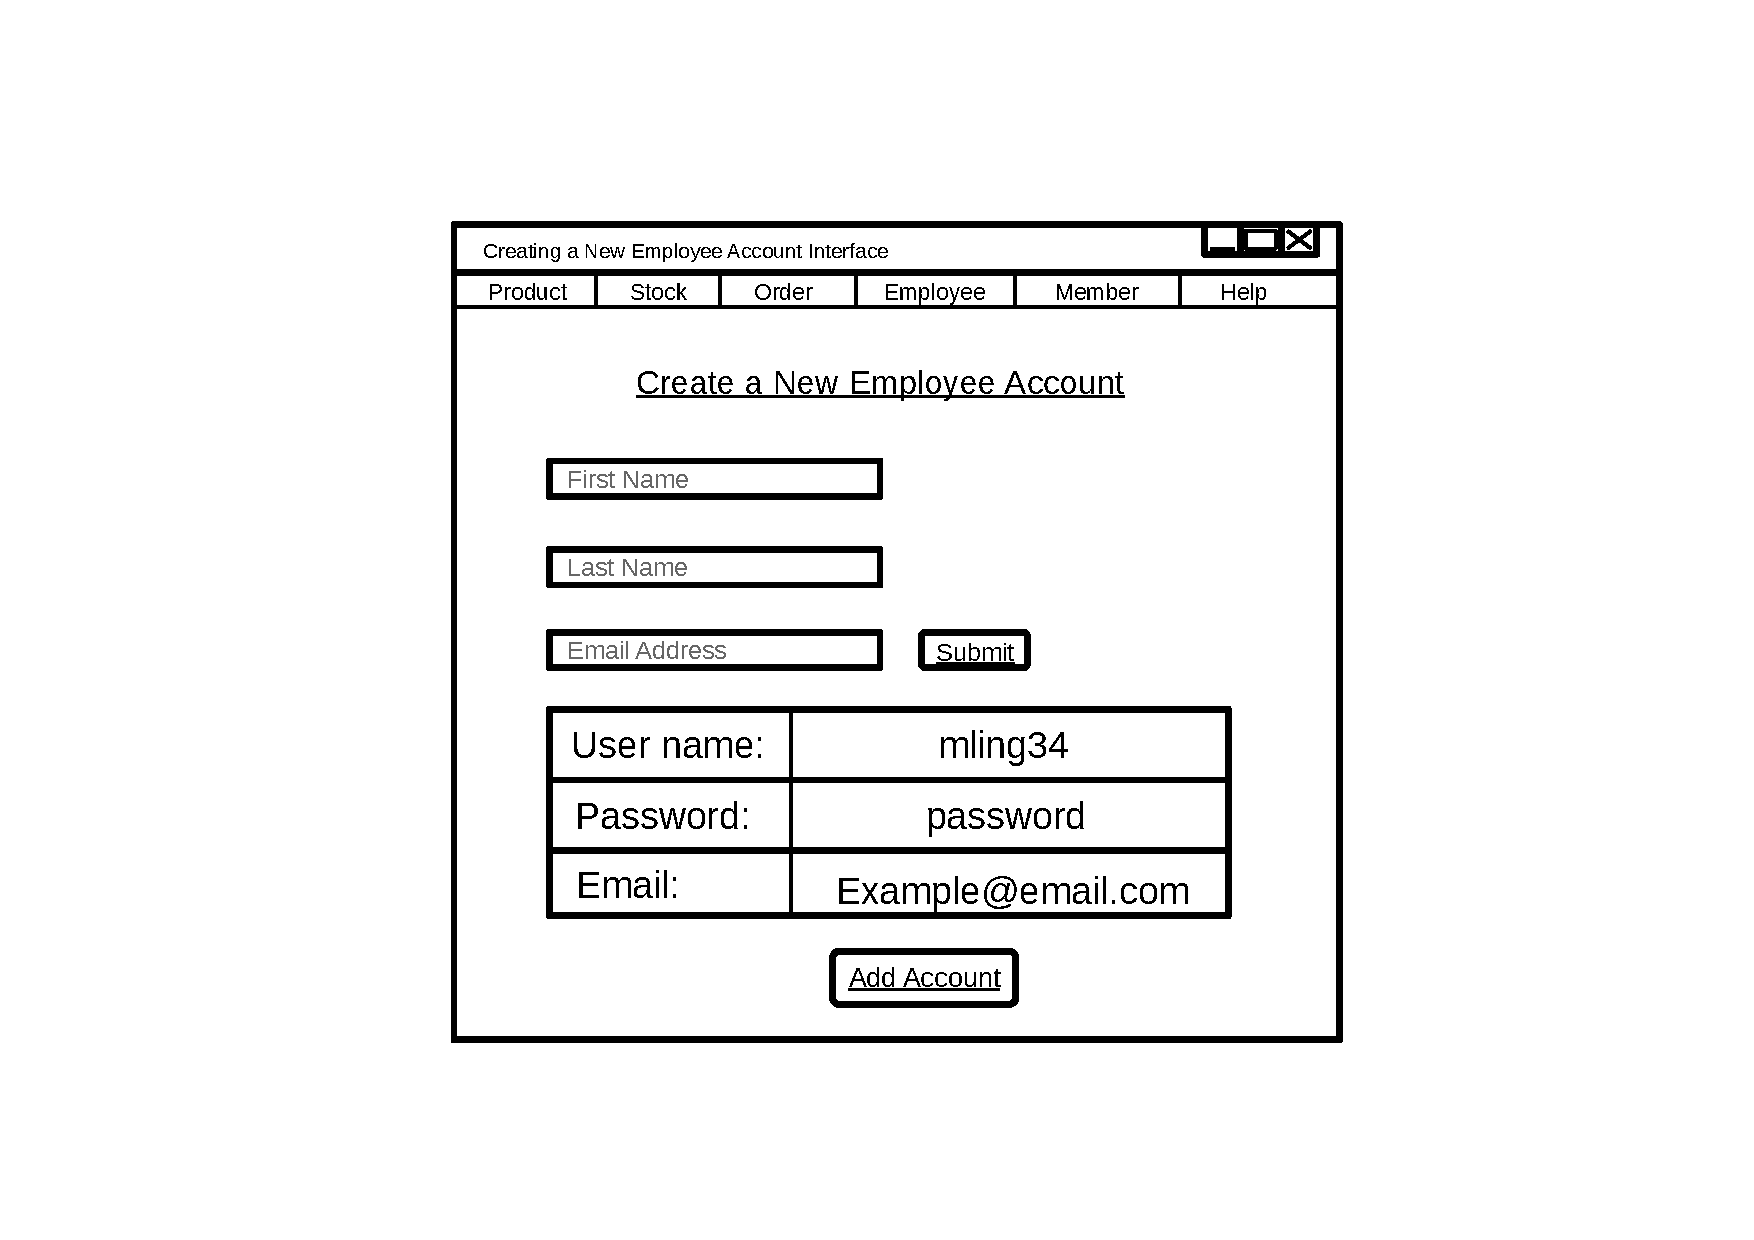
\includegraphics[width = 14cm]{CreatinganEmployeeAccountDiagramEdited.pdf}\hspace*{\fill}
\end{figure}

The `Creating a New Employee Account' interface is very basic. It contains three fields in which the user enters the first name, last name and email address. Once the user has entered the details they can click the `Submit' button. Clicking the `Submit' button will the display the information in the table which will allow the user the review the information they have entered and make changes where necessary. Once the user has entered the correct information they can click the `Add Account' button. This button will then add a new employee to the system with the attributes entered by the user. \par

For security, this interface should only be accessible by my client (the administrator) so employees cannot create and delete other employees. If an Employee that is not an administrator is logged on, the option for add Employee and delete Employee should be grayed out and an appropriate message should be displayed in the drop down menu, telling the user why they cannot access this area of the system. \par

\begin{figure}[H]
\caption{Adding a New Member} \label{fig:Adding a New Member Interface}
\hfill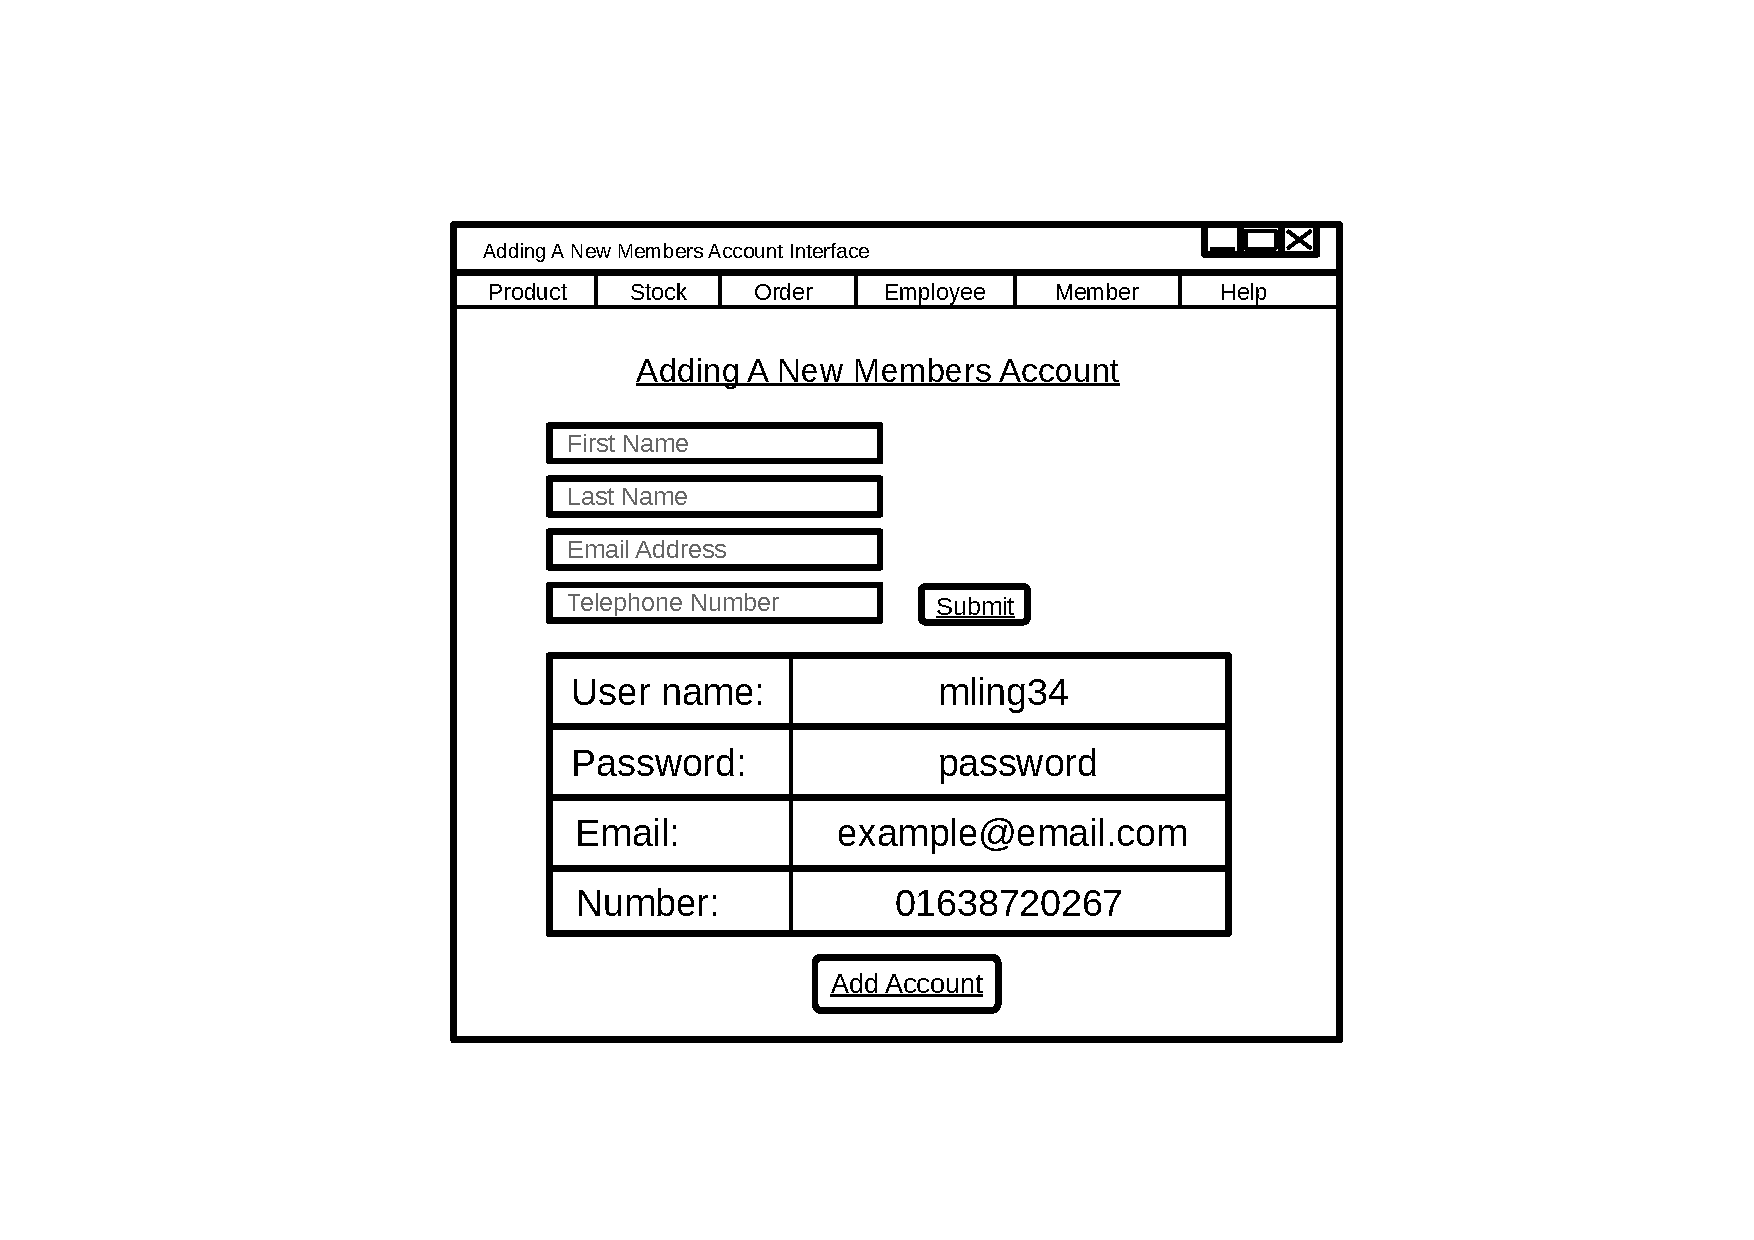
\includegraphics[width = 14cm]{CreatingaMemberDiagramEdited.pdf}\hspace*{\fill}
\end{figure}

Adding a new Member is almost identical to adding a new Employee, however, the user must also enter the member's telephone number. When the user clicks the `Submit' button the information is displayed in a table and the new account is created once the `Add Account' button is pressed. Both the Add a New Member and Add a new Employee interfaces have a large underlined title at the top of the interface. This is to prevent the user from entering the wrong details into the wrong interface. For example the user might accidentally enter a Members information into an Employee Account. The title at the top of each interface is to prevent the suer from choosing the wrong interface. \par

\begin{figure}[H]
\caption{Stock Management Interface} \label{fig:Stock Management Interface}
\hfill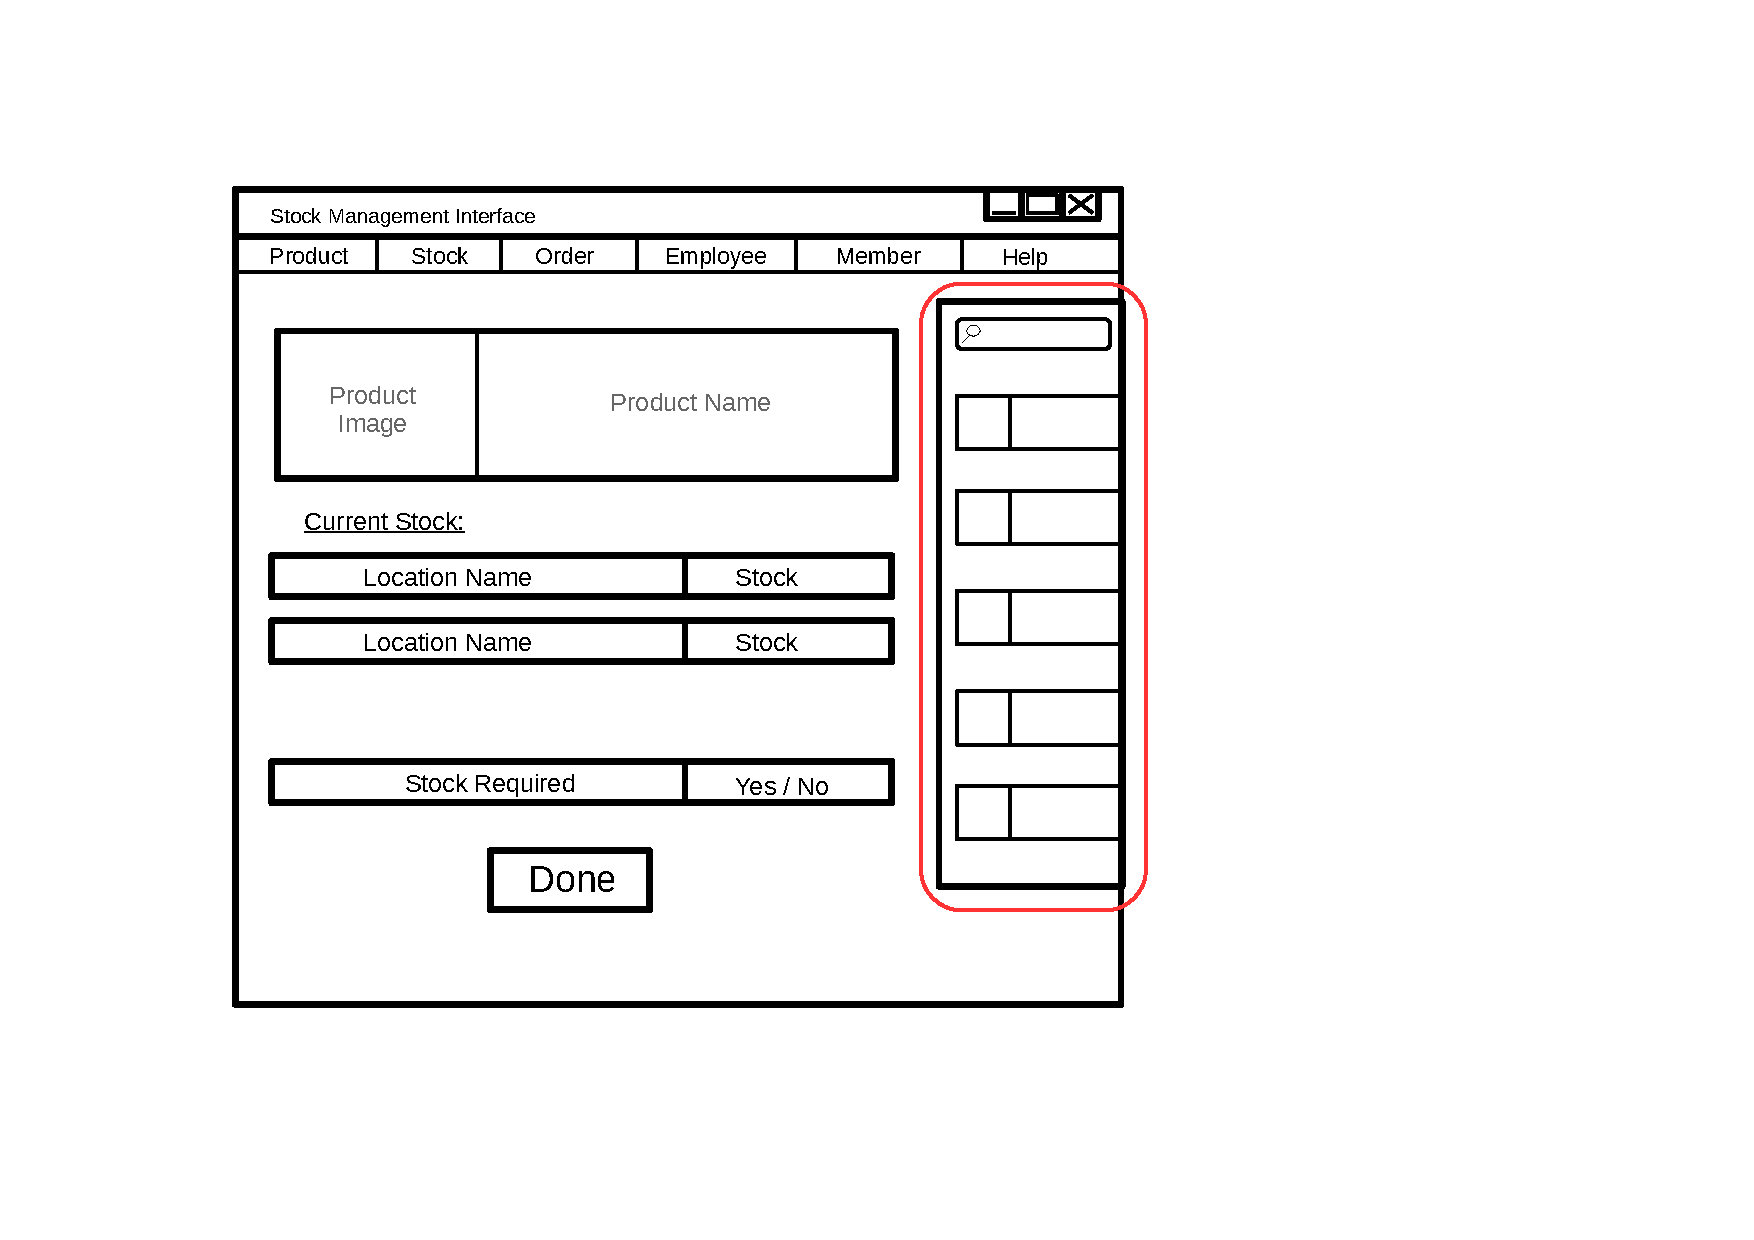
\includegraphics[width = 14cm]{StockManagementDiagramEdited.pdf}\hspace*{\fill}
\end{figure}

Figure 2.19 shows both the Stock Management Interface, but also the search bar. The search bar is circled in red in Figure 2.19, and can be accessed from any of the interfaces other than the log in interface. The search bar allows the User to search for a Product, Employee or Member by entering a string of characters that matches inforamtion stored in the database. for example, entering `food' into the search bar will return any Product with the term `food' in it. \par

  When a match / multiple matches have been found to what is entered into the search field, An image of the product is displayed along with the product name. If the results contain a member or an employee, no image is displalyed just the First and Last name of the member / employee. This sidebar will be accessed using a keyboard shortcut for ease of access and speed of use. \par


\begin{figure}[H]
\caption{Stock Management Interface} \label{fig:Stock Management Interface}
\hfill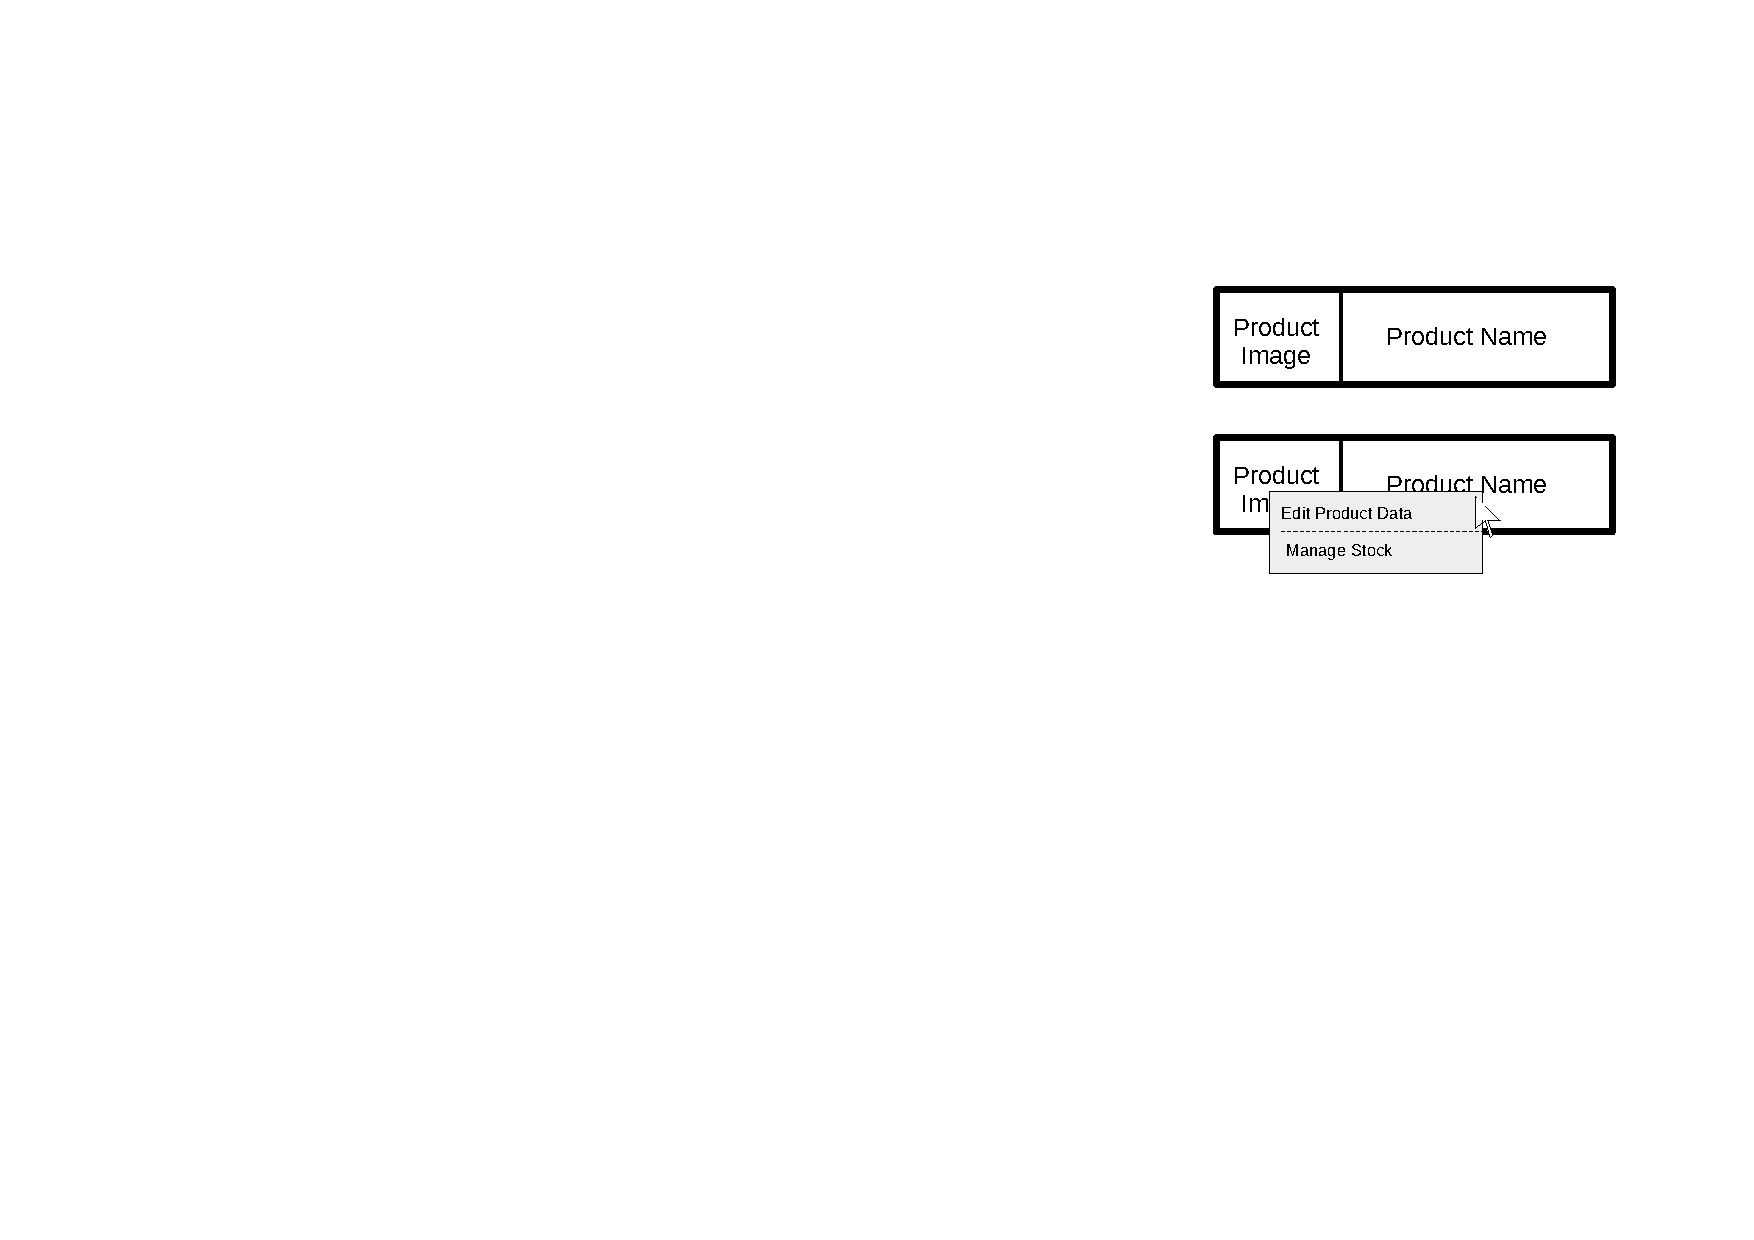
\includegraphics[width = 7cm]{StockManagementDiagramRightClick.pdf}\hspace*{\fill}
\end{figure}

Once the user finds the product they were looking for, they can right click the Product Name or the image and a drop down menu will appear. The user can then either Edit the Product Data or Manage the stock of that specific product. The information about a member is not liekly to change often, but is still possible, therefore, when the user right clicks on the member returned from the search, a similar drop down menu will be displayed and the user will be able to edit the Members details. \par

Going back to Figure 2.19. The stock Management Interface displays the image and name of a product and wil also display the current stock in each location and a will display a boolean variable if more stock of that product is required. The user can change the stock in each location by double left clicking the current stock, which will allow the user to delte the old stock and enter the new stock. Once the user has edited the stock they can hit the `Done' button which will return them to the Product Search Interface.\par

The user will not be able to change the products image or name here. This can be done by going to the Product tab and selecting Edit Product Data. This will take the User to the `Add a new Product Interface, however the information will already be filled out with the information the product the user wants to edit. The user can then change the attributes they want and save the Product with the changed data. 

\subsection{Hardware Specification}
	
The hardware specifications for my clients current computer are: \par

\begin{itemize}
\item Windows 7 Home Edition
\item Intel® Core™ i3-3240T Processor (2.9 GHz)
\item 4 GB DDR3 RAM
\item 1 TB HDD, 7200 rpm
\end{itemize}




I have decided that my client does not mandatory need to purchase any further hardware in order to run my new system. This is because my client's hardware is more than capable of running my new system. Therefore, there shall be no cost for new hardware. My client's hardware is suitable for the purpose of my new system, the processor will be more than capable of running my system. However the computer is roughly 3 years old, meaning that errors within the registry may have occurred which over time slows down the speed of the computer. This factor may or may not effect the speed in which my client can use my new system. My client has more than enough memory to run my system by itself. However, my client may or may not encounter small speed issues when using the system whilst other applications are running such as Google Chrome etc \ldots However most normal programs will not have a major effect the speed of the computer.  My client has a large 1 Terra-byte Hard Disk Drive. The size of this drive is more than capable of storing all of the data within my system. My client does not have to make any mandatory hardware changes, however they may wish to make optional changes to improve the overall performance of the system. my client could purchase a new processor with equal or higher clock speeds, which may increase the overall speed of the computer depending on how old the computer is.  my client could also replace the 1TB Hard Disk Drive with a Solid State drive, this increases the Read / Write speeds of the data stored on the drive as the information is stored in flash memory chips as apposed to magnetic coating on a platter. This means the information can be transfered much faster. However, solid state drives have an extremely high cost compared to Hard disk drives. These changes will be unnecessary and almost unnoticeable.

\section{Program Structure}


\subsection{Top-down design structure charts}

\begin{landscape}
\begin{figure}[H]
\caption{Changing Stock Structure Chart} \label{fig:SotckStructureChart}
\hfill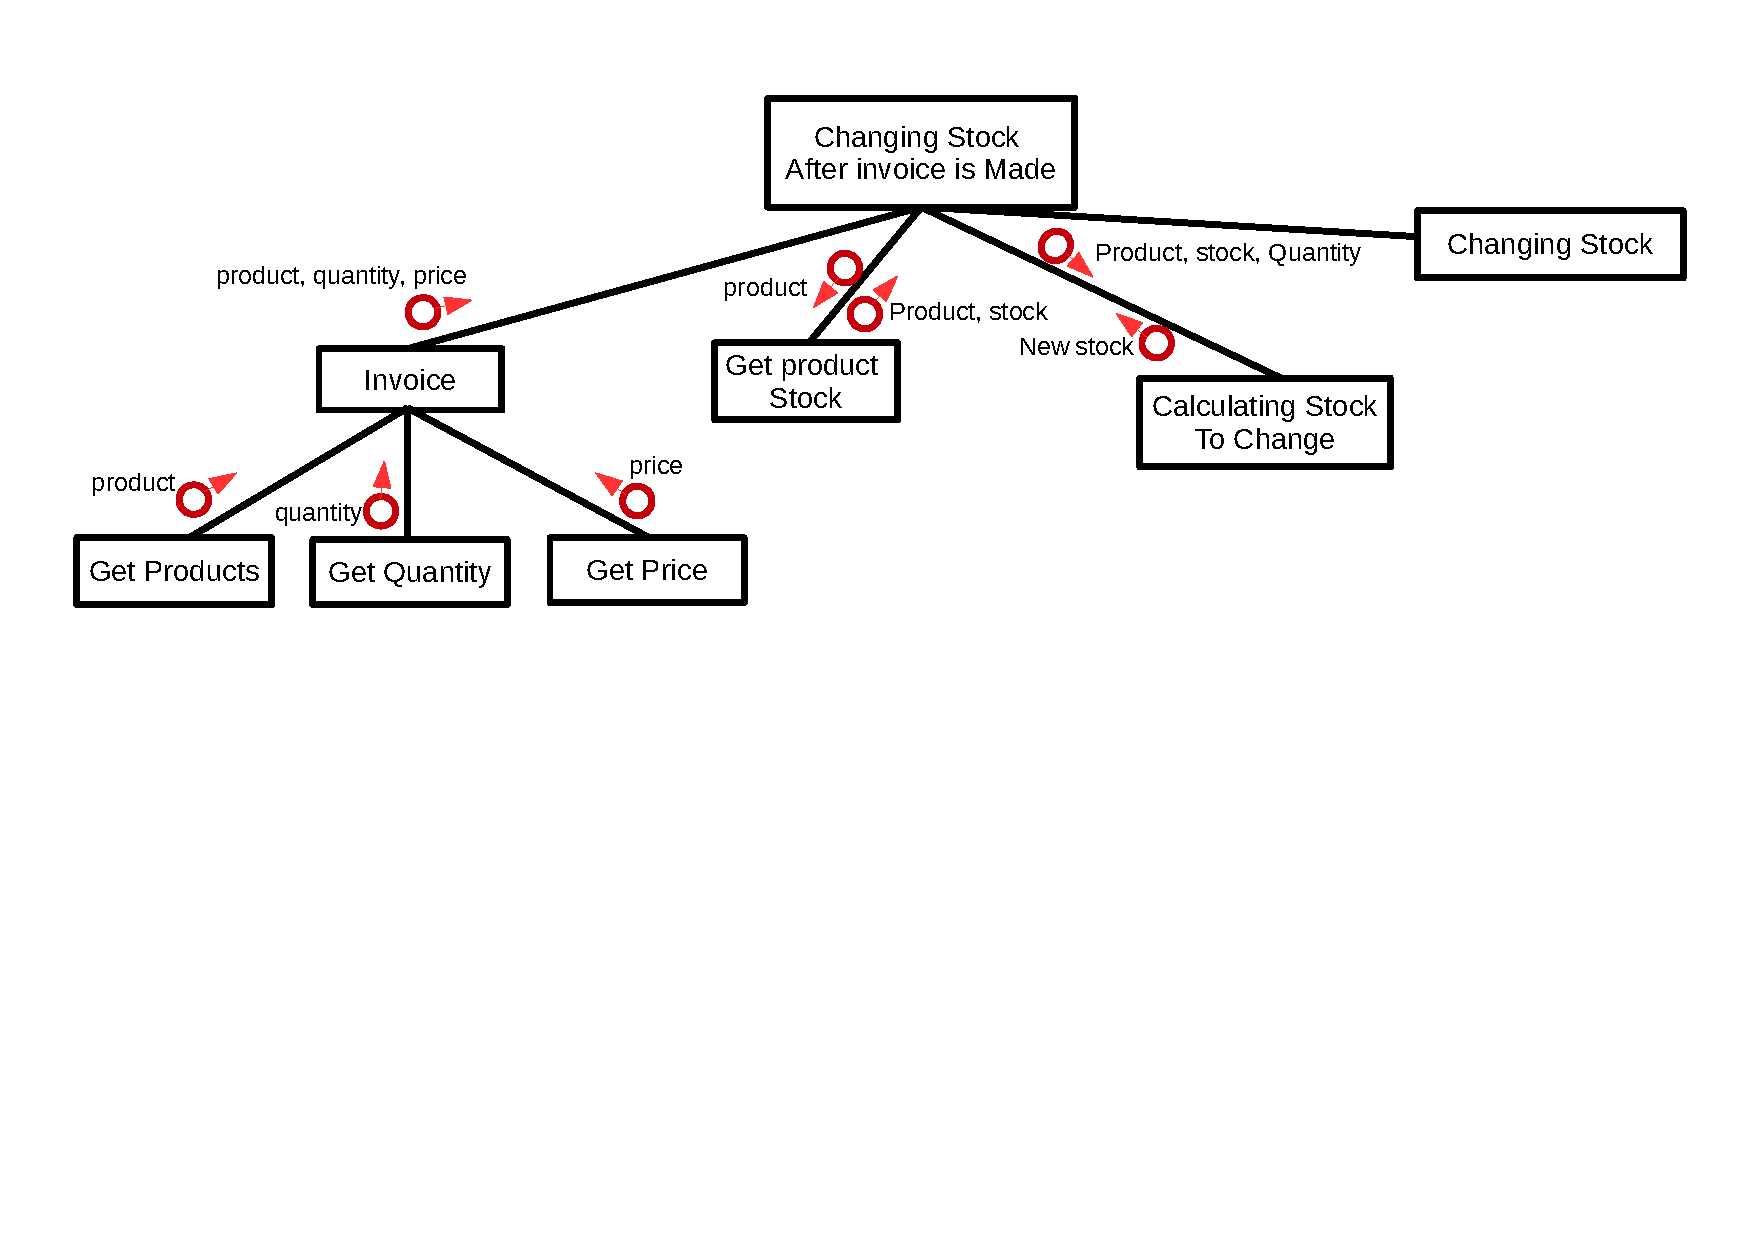
\includegraphics[scale=0.65]{TDSC1.pdf}\hspace*{\fill}
\end{figure}



\begin{figure}[H]
\caption{Password Reset Structure Chart} \label{fig:PasswordStructureChart}
\hfill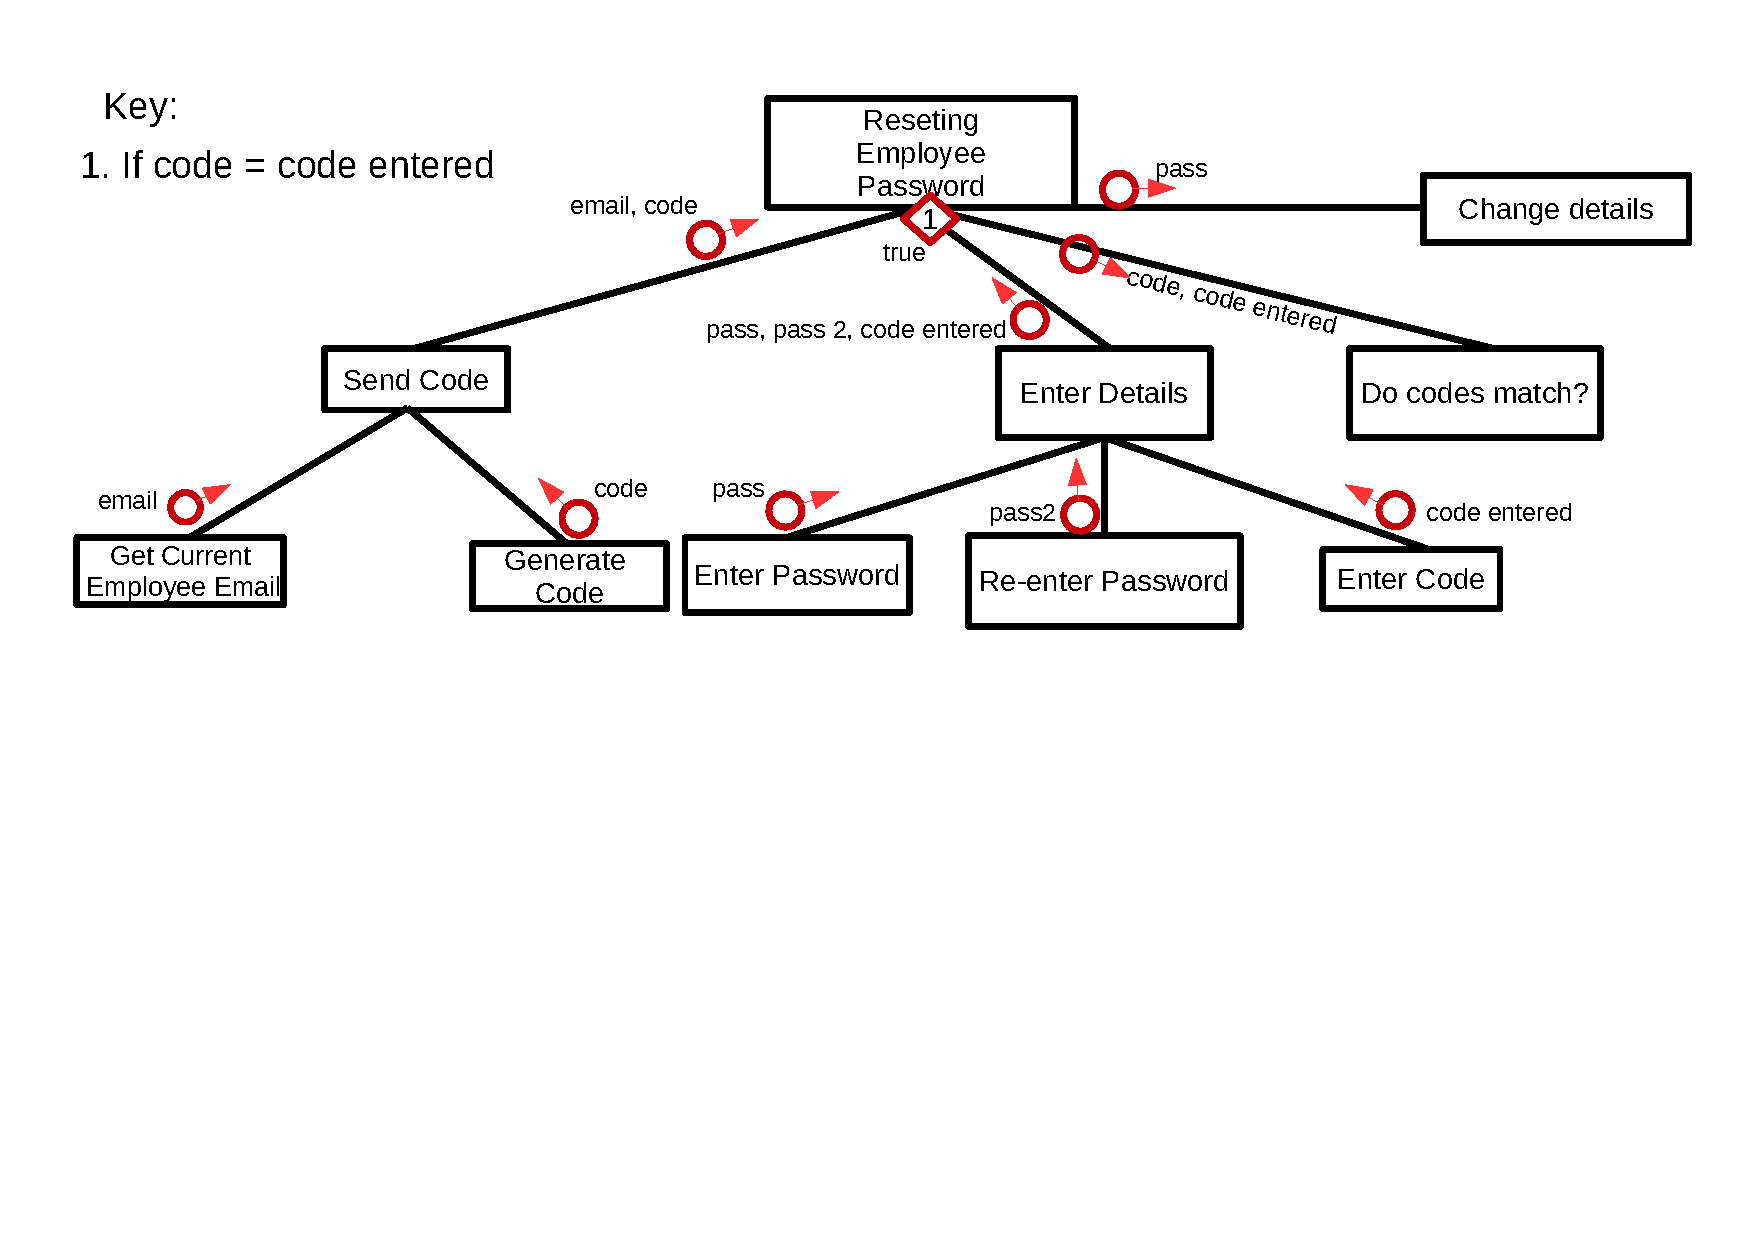
\includegraphics[scale=0.65]{TDSC2.pdf}\hspace*{\fill}
\end{figure}
\end{landscape}


\subsection{Algorithms in pseudo-code for each data transformation process}
\begin{algorithm}[H]
\label{fig:repeat_pseudo_example}
\caption{Adding A New Product}
\begin{algorithmic}[1]
\SET{$ProductName$}{$NameOfProduct$}
\SET{$ProductID$}{$Product_List[ProductID]$}
\SEND{$"Does\ the\ product\ have\ a\ specific\ Size"$}
\RECEIVE{$Size$}
\If{$Size = "Yes"$}
\SEND{$Enter\ The\ Size\ Of\ The\ Product$}
\RECEIVE{$Size$}
\SET{$ProductSize$}{$ProductSize$}
\EndIf
\SET{$ProductQuantity$}{$QuantityOfProductInStock$}
\SET{$ProductPrice$}{$PriceOfProduct$}
\SEND{$"Is\ The\ Price\ of\ the\ product\ been\ reduced\ (On Offer)"$}
\RECEIVE{$Reduction$}
\If {$Reduction > 0$}
\SET{$ProductPrice$}{$ProductPrice * (Reduction / 100)$}
\EndIf 
\end{algorithmic}
\end{algorithm}

\begin{algorithm}[H]
\label{fig:repeat_pseudo_example}
\caption{Adding The Product to The Database}
\begin{algorithmic}[1]
\Function {AddProduct}{ProductName: NewProductName, Category: NewCategory, Price: NewPrice}
\For{$Product$ in $ProductList$ DO}
	\SET{$ProductID$}{$ProductID+1$}
\EndFor
\SET{$ProductName$}{$NewProductName$}
\SET{$Category$}{$NewCategory$}
\SET{$Price$}{$NewPrice$}
\SEND{$Product(ProductID, NewProductName, NewCategory, NewPrice) to ProductDatabase$}
\EndFunction
\end{algorithmic}
\end{algorithm}




\begin{algorithm}[H]
\label{fig:repeat_pseudo_example}
\caption{Searching For a Product}
\begin{algorithmic}[1]
\Function {SearchForProduct}{ProductName: ProductName}
\SET{Count}{0}
\For{Product in ProductList DO}
	\If{$ProductName = ProductName'$ }
		ProductList[Count] = Product
	\EndIf
\EndFor
\EndFunction
\end{algorithmic}
\end{algorithm}


\subsection{Object Diagrams}

\begin{figure}[H]
\caption{Object Diagram} \label{fig:Object Diagram}
\hfill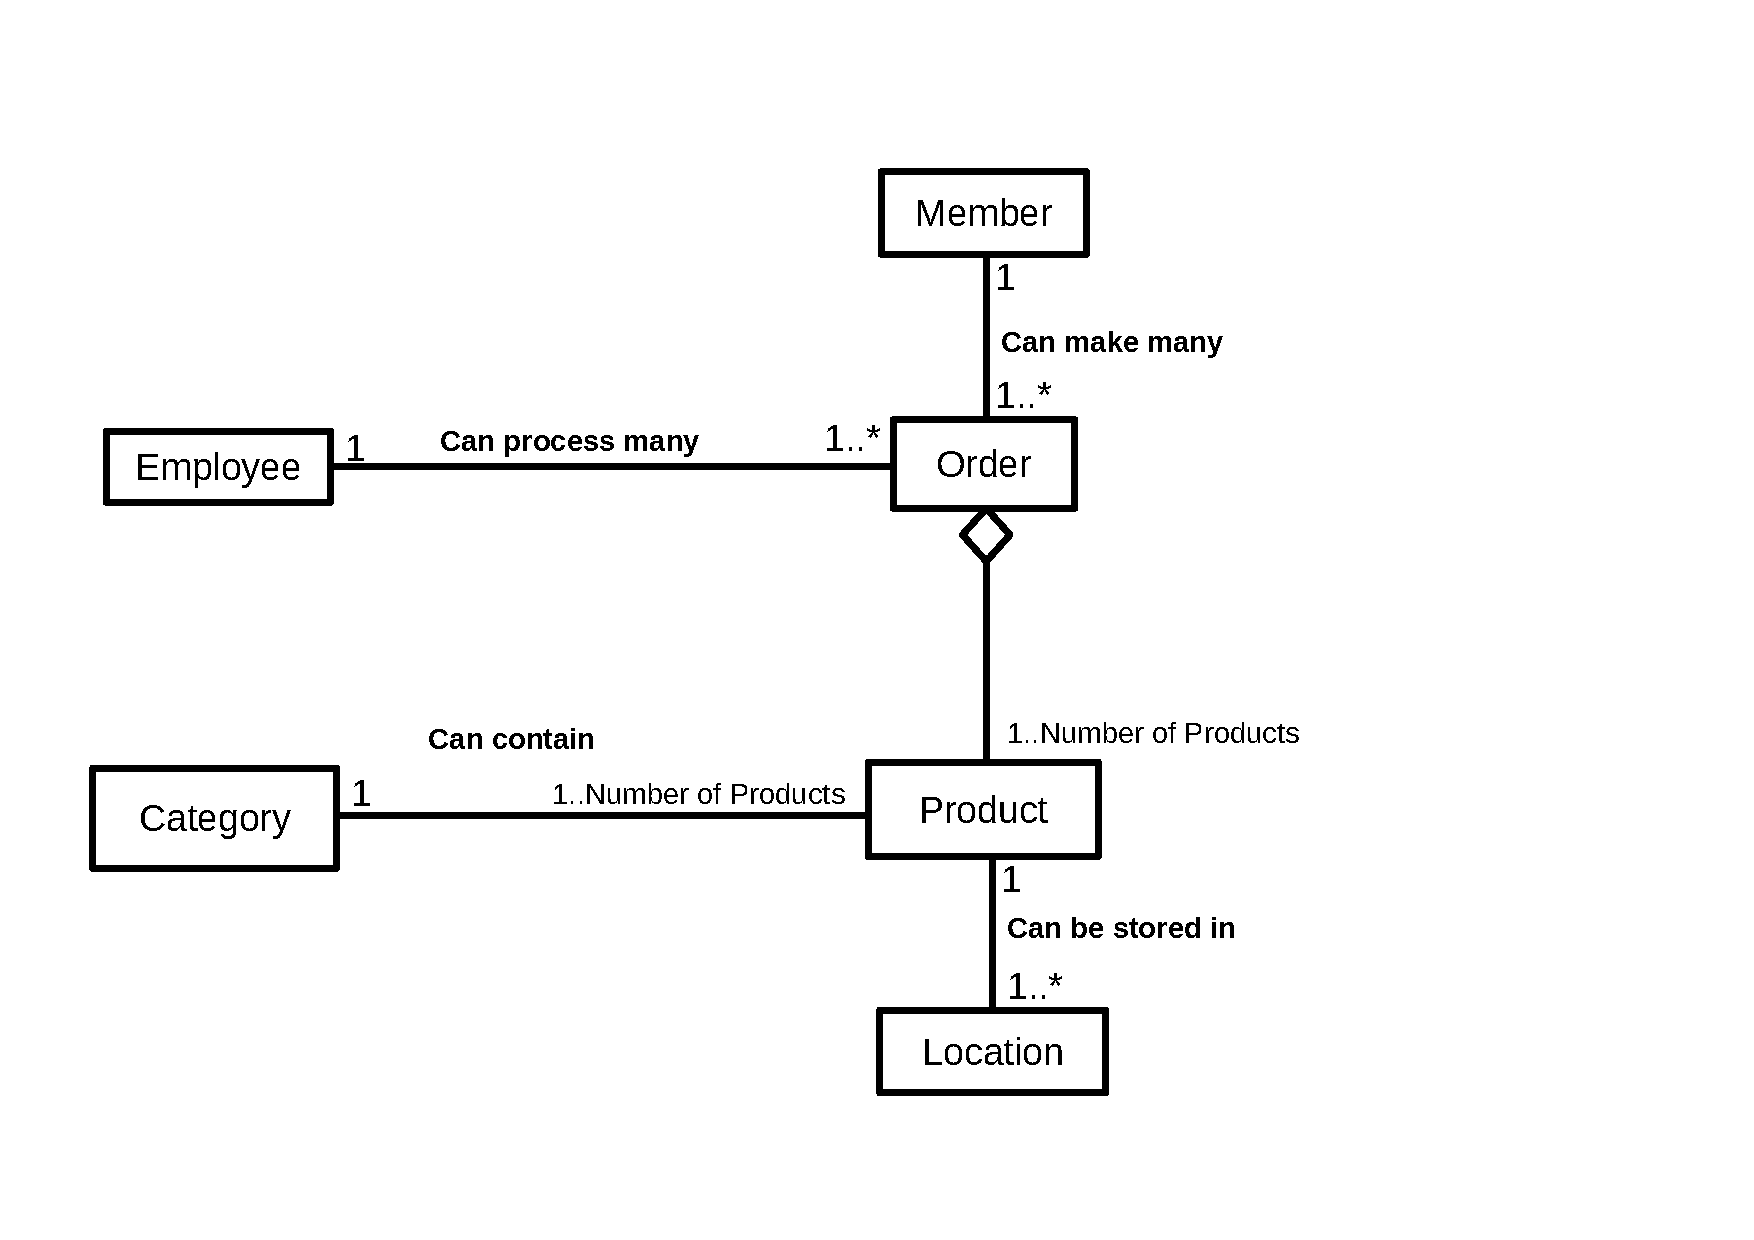
\includegraphics[scale=0.65]{ObjectDiagram.pdf}\hspace*{\fill}
\end{figure}

\subsection{Class Definitions}

\section{Prototyping}

When a user tries to reset their password, there must be a level of verification so that only the User of that account can change the password. Therefore, in my system i wanted to implement a method where if the user would like to reset their password, an email is sent to the email address associated with that Employee Account. This was a problem as i did not know how to send emails through python. \par

After doing some research, i learnt how to send an email from a gmail account to any other email address. When the program below is run, an email is sent to any email address containing a code.

\begin{python}
import smtplib
import random

code = random.randint(1000,9999)
print(code)

content = '{0}'.format(code)

mail = smtplib.SMTP('smtp.gmail.com','587')

mail.ehlo()

mail.starttls()

mail.login('mattling147@gmail.com', password)

mail.sendmail('mattling147@gmail.com','mattling9@hotmail.co.uk',content)

mail.close()

\end{python}

The Code is a 4 digit random number between 1000-9999. this number is generated on line 4 by using the built in `random' function in python. Line 7 then adds the code to the content of the email. To send an email the email and password of an existing gmail account must be entered on line 15. line 17 , (mail.sendmail), contains the Sender Email, The recipient Email and the Contents of the email. The contents of the email is the code generated on line 4, the Sender email is the gmail account that is logged in on on line 15 and the Recipient Email is the email of the employee that is requesting to change their password.


\begin{figure}[H]
\caption{Results From Test 1} \label{fig:Results From Test 1}
\hfill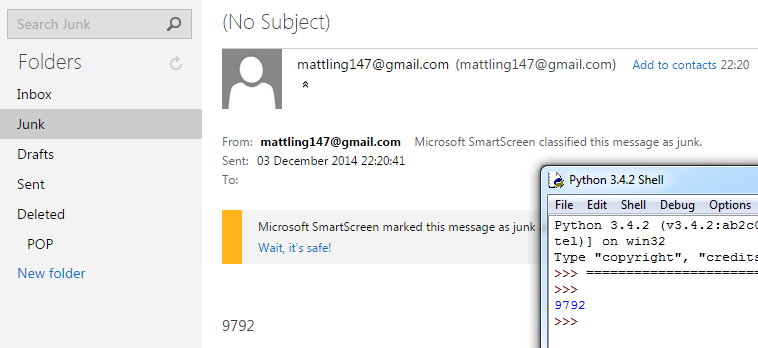
\includegraphics[width = 15cm]{EmailTestEvidence.png}\hspace*{\fill}
\end{figure}


Figure 2.15 shows the results form the first prototype. The `9792' in blue is the code genrated by the random number generator, and i displayed it in the program to ensure it matches the code sent in the email. Looking at the email, i can see that the codes successfully match, however there are a few issues with this prototype. The first issue is that the email is sent with No Subject. This is a problem as it maybe hard for the employee to find the email if it has no subject. Another issue with having no Subject, is that the email has been sent to the junk. This is a problem because the user may expect the email to be received in their inbox as apposed to their junk. Another small problem is that the content of the email is not very user friendly, it simply contains the 4 digit code. \par

\pagebreak

I undertook a second investigation to try fix the problems found in the first investigation. In my second investigation, i found that a message can be formatted so that the To:, From: and Subject can be specified. This is shown from lines 7 - 13 in the Code below.

\begin{python}
import smtplib
import random

code = random.randint(1000,9999)
print(code)

msg = "\r\n".join([
  "From: BeaconVets@Admin.com",
  "To: mattling9@hotmail.co.uk",
  "Subject: Password Reset Link",
  "",
  ("{0}{1}".format("Hello User, \n \n Your Reset Password Link is:  ",str(code)))
  ])

mail = smtplib.SMTP('smtp.gmail.com','587')

mail.ehlo()

mail.starttls()

mail.login('mattling147@gmail.com', password)

mail.sendmail('mattling147@gmail.com','mattling9@hotmail.co.uk',msg)

mail.close()

\end{python}

I gave the subject an appropriate name so that the employee can easily find the email if they search their inbox for it. On Line 12 i have changed the content of the email form just being the four digit code, to greeting the user and describing to the user what the code is for. \par

\begin{figure}[H]
\caption{Results From Test 2} \label{fig:Results From Test 2}
\hfill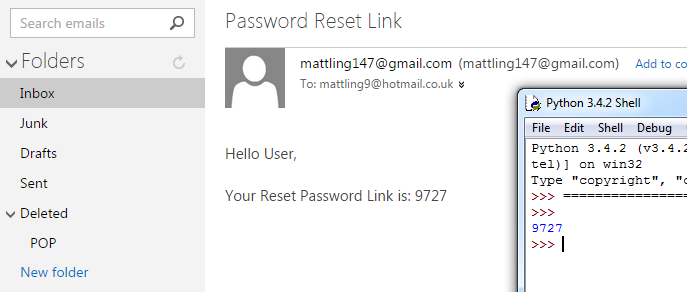
\includegraphics[width = 15cm]{EmailTestWithSubjectEvidence.png}\hspace*{\fill}
\end{figure}

Looking at Figure 2.16 we can see that our problems have been resolved. The email now has a Subject of `Password Reset Link'. The email has also been received in the users inbox rather than their junk, and the content of the email is more user friendly. This Prototype can now be implemented into my system with a few modifications to work with my system. One small improvement that could be made is that the Code could be Displayed in Bold within the email so that it is easily distinguishable between the other text. \par
\pagebreak


A simple test i needed to do, was to find out how to make a button clickable or not, depending on the state of a checkbox. Below is an example of what i want to implement into my system:

\begin{figure}[H]
\caption{Results From Test 2} \label{fig:Results From Test 2}
\hfill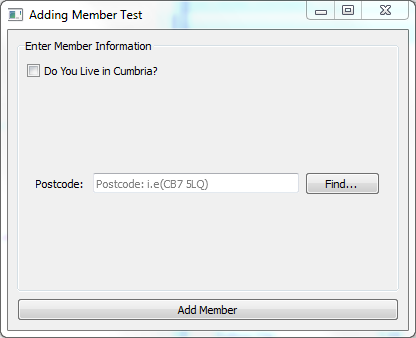
\includegraphics[width = 15cm]{ToggleFindBefore1.png}\hspace*{\fill}
\end{figure}

Here, the tickbox is currently not checked. When the tickbox is not checked i do not want the button to be clickable. However when the user checks the checkbox, i want the button to become clickable. This means that i am going to have to connect a method to the checkbox when it is clicked.
\begin{python}
self.postcode_tickbox.stateChanged.connect(self.change_button_method)
\end{python}
The line above runs the change_button_method whenever the the state of the checkbox is changed (whenever it is checked or unchecked.) In the change_button_method, i need to determine the current state of the checkbox, in order to know whether to change the button to clickable or not clickable.

\begin{python}
self.postcode_tickbox.checkState()
\end{python}

when run, the line above will return true if the checkbox is checked or will return false if the box is not checked. I will also need to change the button to clickable or not clickable. The code below is how to do it.

\begin{python}
self.find_button.setEnabled(False)
\end{python}

When set to False, the button is not clickable, however when set to True, the button becomes clickable. Finally i need to add an IF statement to say for example, IF the checkbox is currently checked, change the push button so it is clickable. The final working IF function is displayed below within the "change_button_method" method.

\begin{python}
def change_button_method(self):
        if self.postcode_tickbox.checkState() == False:
            self.find_button.setEnabled(False)
        else:
            self.find_button.setEnabled(True)
\end{python}

this now changes the state of the push button depending on whether the checkbox is checked or not. Below is evidence of the test sucessfully working:

\begin{figure}[H]
\caption{Results From Test 2} \label{fig:Results From Test 2}
\hfill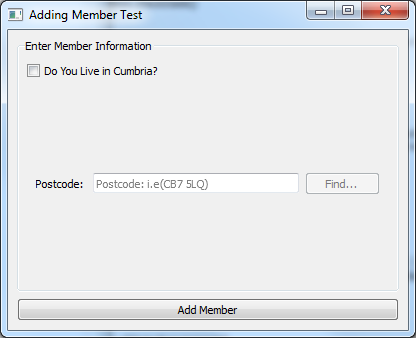
\includegraphics[width = 15cm]{ToggleFindAfter1.png}\hspace*{\fill}
\end{figure}

\begin{figure}[H]
\caption{Results From Test 2} \label{fig:Results From Test 2}
\hfill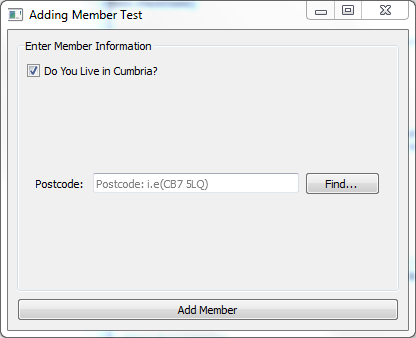
\includegraphics[width = 15cm]{ToggleFindAfter2.png}\hspace*{\fill}
\end{figure}

The User will be able to click the checkbox if they live in Cumbria. They can then enter their postcode and click the find button. Once they click the find button i want the system to be able to find information about their location and to be able to automatically fill it in for them i.e their town, street ect. In order to do this i will need an Array of data containing The relevent information for each postcode. Creating this large array manually in Python is a bad idea as it would take an enormous amount of time and would be an incredibly tedeous process.

 Instead, i did some research and found a CSV File online containing The Postcode, Latitude, Longitude, Town and County of every location in england. This file was 500Mb, which i felt was too large to store the information about every postcode in england.Therefore, i decided just to use the postcodes in Cumbria because this is where the business is situated and where the vast majority of the customers will be from. I removed the columns containing the Longitude and Latitude of the location as this information will not be relevent within my system.After removing The irellivent postcodes and information the file size was reduced to 556Kb. The screenshot below shows what the CSV looks like:

\begin{figure}[H]
\caption{Results From Test 2} \label{fig:Results From Test 2}
\hfill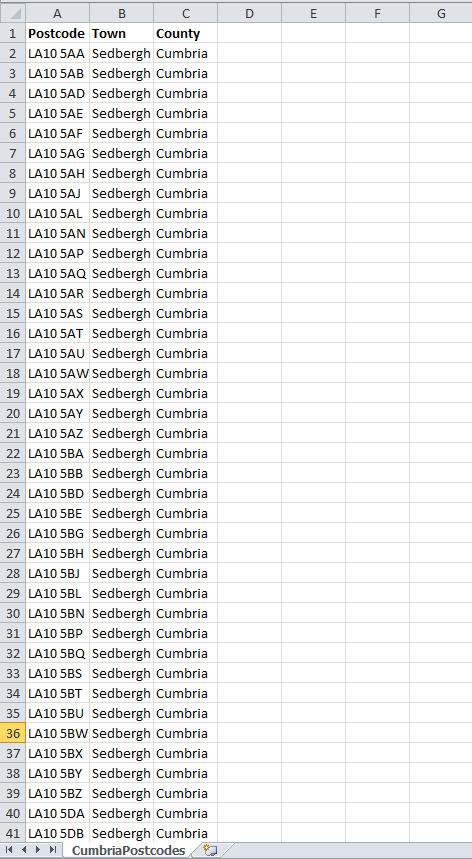
\includegraphics[width = 15cm]{PostcodeScreenshot.png}\hspace*{\fill}
\end{figure}

I want my system to be able to see if the postcode the user entered is in the file, and if it use, use the corresponding data to fill out the Town and County automatically. In order to use the data in the CSV file i have to import the csv module in python. This is doen simplying by doing \begin{python} import csv \end{python} Then, in order to use the data within the file i use the line:

\begin{python}
with open("CumbriaPostcodes.csv", "r")as postcode_file:
                        self.postcodes = csv.reader(postcode_file)
                        for item in self.postcodes:
                                self.address_list.append(item)
\end{python}

The code above opens the CSV file.  \begin{python} "with open("CumbriaPostcodes.csv", "r")as postcode_file:"\end{python} Tells python that it needs to open the file "CumbriaPostcodes.csv", which is the name of the file containing the postcodes and the "r" tells python that i only want to read the data from it. If i wanted to add data i could use either "a" or "w".  \begin{python} "self.postcodes = csv.reader(postcode_file)"  \end{python} assigns self.postcodes to the postcode file. The data within the csv can now be used in python. I now want to Add each Address (Postcode, County and Town) to a list to create an Array. This is done simply by saying:

\begin{python}
 for item in self.postcodes:
                                self.address_list.append(item)
\end{python}

This says that for every line in the csv file, add that line to the self.address_list list. Using self.postcode_entered as the variable that contains the string of the postcode the user enters, I can see if that postcode is in the file by doing:
\begin{python}
for count in range(0, len(self.address_list)):
                                if self.postcode_input in self.address_list[count]:
\end{python}

The FOR loop is run once for each item in the list. In this case its 19,363 times. Then for each address, it checks whether the postcode the user entered matches the postcode for that address. If they do match i want the system to get the county and town and then insert that data to the data fields. If the postcodes do not match, it should move to the next address in the array. If the postcode doesn't match any of the postcodes, an appropriote message should be displayed. The following code simply Assigns the County and Town from the CSV File to the County and Town Data Fields in my system if the postcodes match:

\begin{python}
self.index = self.county.findText(self.address_list[count][2])
                                        self.county.setCurrentIndex(self.index)
                                        self.town.setText(self.address_list[count][1])
\end{python}

self.county is a combo box containg all the counties in England. The user simply selects the county from the list. \begin{python}"self.index = self.county.findText(self.address_list[count][2])" Looks in the county combo box and finds the index of the County that matches the postcode, this index is then assigned to self.index.\begin{python}  "self.county.setCurrentIndex(self.index)" \end{python}simply changes the current index of the combo box to the index of the matching county. Because self.town is a line edit, this can just be directly assigned to the town from the matching address. This is done using:\begin{python}"self.town.setText(self.address_list[count][1])".\end{python} Below is the working example of the test working:

Here we can see that 'CA7 4QT' is a legitimate postcode in the csv file.

\begin{figure}[H]
\caption{Results From Test 2} \label{fig:Results From Test 2}
\hfill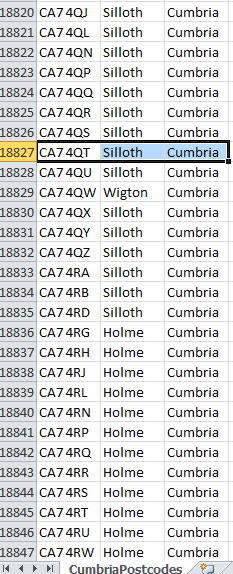
\includegraphics[width = 15cm]{FindingPostcodeEvidence1.png}\hspace*{\fill}
\end{figure}

The postcode is then entered into the postcode field, the checkbox is ticked which enables the find button and the find button is clicked. The find button is connected to the "find_postcode_method" method. Once the button is clicked, you can see that the data fields have been changed correctly. The fields highlighted in green shows that the data is valid.

\begin{figure}[H]
\caption{Results From Test 2} \label{fig:Results From Test 2}
\hfill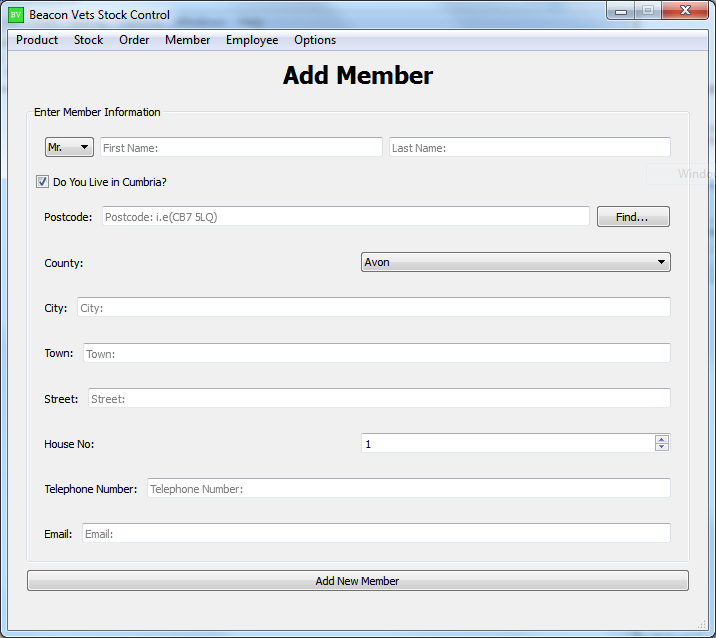
\includegraphics[width = 15cm]{FindingPostcodeEvidence2.png}\hspace*{\fill}
\end{figure}

\begin{figure}[H]
\caption{Results From Test 2} \label{fig:Results From Test 2}
\hfill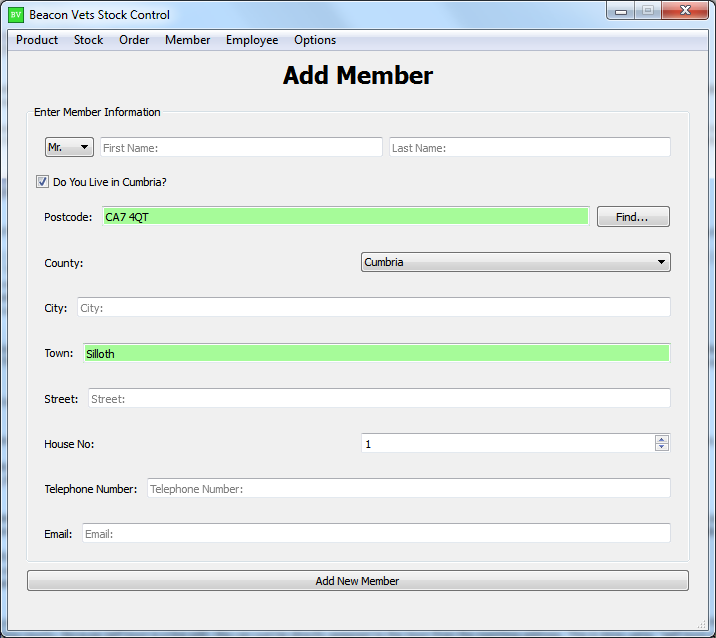
\includegraphics[width = 15cm]{FindingPostcodeEvidence3.png}\hspace*{\fill}
\end{figure}

Another test which i had to prototype was when An image is assigned to a specific product, a copy of that image is stored in my system so if the user deletes the image, there will be a copy of it that the system can use. 

An easy way to make a copy of a file in python is to use the Shutil module. to use this module, i simply imported it using "import shutil". using the method "shutil.copy()" you simply enter the path in which the file comes from including the file name, and then the new path including the new name of the file. To implement this into my system, i use a Dialog box to get the image path from the user, then use the path to copy the image. because im storing all the product images in the same folder, the path the images are going to will be the same. Each image will be named as its associated products ProductID, i.e (15.jpg). Below is a working example of the code where self.path.text() is the original path of the image, supplied by the user and the new path is the folder in which the files are stored.

\begin{python}
path = self.path.text()
new_path = "./ProductImages/01.jpg"
shutil.copy(path, new_path)
\end{python}

The last simple thing that i wanted to prototype was to ensure the postcode is legitimate before it is added. In order for the postcode to be valid it must follow a specific pattern of letters and numbers. I used a regular expression to validate the postcode. to use regular expressions, i simply imported the regular expression module: \begin{python}"import re".\end{python} then to create a regular expression i just did:
\begin{python}
self.pattern = re.compile("[A-Z]{1,2}[0-9][0-9A-Z]?\s?[0-9][A-Z]{2}")
\end{python}
 The regular expression above says that the postcode must have between 1 and 2 letters between A and Z, followed by an number between 0 and 9, then followed by either a number or a letter. after this the postcode must have a space then finally must end with a number between 0 and 9 and 2 letters between A and Z.

to insure the postcode was between A and Z not a and z i used \begin{python}" postcode = postcode.upper()" \end{python}. this simply capitalized all the letters in the postcode.

Below is an exmaple of a valid and a non valid postcode, if the postcode is valid, the system changes the background of the line edit from white to green.

\begin{figure}[H]
\caption{Results From Test 2} \label{fig:Results From Test 2}
\hfill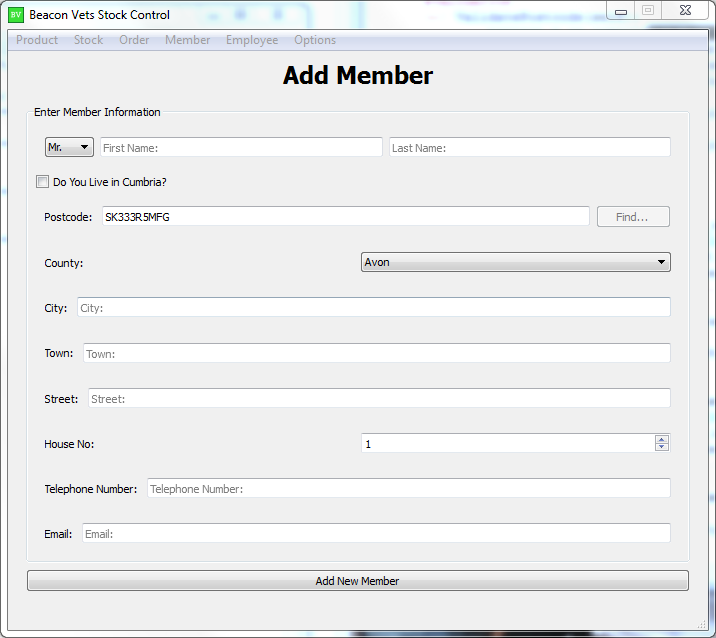
\includegraphics[width = 15cm]{ValidationTest1.png}\hspace*{\fill}
\end{figure}

\begin{figure}[H]
\caption{Results From Test 2} \label{fig:Results From Test 2}
\hfill\includegraphics[width = 15cm]{ValidationTest2.png\hspace*{\fill}
\end{figure}


\section{Definition of Data Requirements}

\subsection{Identification of all data input items}

\begin{itemize}
\item Product Name
\item Size
\item Category
\item Employee First Name
\item Employee Last Name
\item Employee Password
\item Employee Email
\item Date
\item Time
\item Title
\item Member First Name
\item Member Last Name
\item House No
\item Street
\item Town
\item City
\item County
\item Postcode
\item Telephone Number
\item Member Email
\item Location Name
\item Stock
\item Employee Username
\item Quantity
\end{itemize}

\pagebreak

\subsection{Identification of all data output items}

\textbf{Output to user}
\begin{itemize}
\item Members First Name
\item Members Last Name
\item Members Email Address
\item Members Telephone Number
\item Employees First Name
\item Employees Last Name
\item Employees Email
\item Product Restock
\end{itemize}

\textbf{Output to Database}
\begin{itemize}
\item Product Name
\item Size
\item Category
\item Employee First Name
\item Employee Last Name
\item Employee Password
\item Employee Email
\item Date
\item Time
\item Title
\item Member First Name
\item Member Last Name
\item House No
\item Street
\item Town
\item City
\item County
\item Postcode
\item Telephone Number
\item Member Email
\item Location Name
\item Product Stock in each Location
\item Employee Username
\item Quantity
\end{itemize}
\subsection{Explanation of how data output items are generated}

  \begin{tabular}{|p{4cm}|p{4cm}|}
        \hline
	\textbf{Output} & \textbf{ How the Output is Generated}\\ \hline
	{Member First Name} & {The Data is displayed so the Member can review the information they have entered whilst creating a new Member}\\ \hline
	{Members Last Name} & {The Data is displayed so the Member can review the information they have entered whilst creating a new Member}\\ \hline
	{Members Email Address} & {The Data is displayed so the Member can review the information they have entered whilst creating a new Member}\\ \hline
	{Members Telephone Number} & {The Data is displayed so the Member can review the information they have entered whilst creating a new Member}\\ \hline
	{Employee First Name} & {The Data is displayed so the Employee can review the information they have entered whilst creating a new Employee}\\ \hline
	{Employee Last Name} & {The Data is displayed so the Employee can review the information they have entered whilst creating a new Employee}\\ \hline
	{Employee Password} & {The Data is displayed so the Employee can review the information they have entered whilst creating a new Employee}\\ \hline
	{Employee Email} & {The Data is displayed so the Employee can review the information they have entered whilst creating a new Employee}\\ \hline
	\end{tabular}
	
	
 \begin{tabular}{|p{4cm}|p{4cm}|}
        \hline
        	{Product Restock} & {If the total stock of a specific product has gotten lower than the minimum stock allowed.}\\ \hline
	{Product Name} & {Employee inputs Information}\\ \hline
	{Size} & {Employee inputs Information}\\ \hline
	{Category} & {Employee inputs Information}\\ \hline
	{Employee First Name} & {Employee inputs Information}\\ \hline
	{Employee Last Name} & {Employee inputs Information}\\ \hline
	{Employee Password} & {Employee inputs Information}\\ \hline
	{Employee Email} & {Employee inputs Information}\\ \hline
	{Date} & {Employee inputs Information}\\ \hline
	{Time} & {Employee inputs Information}\\ \hline
	{Title} & {Employee inputs Information}\\ \hline
	{Member First Name} & {Employee inputs Information}\\ \hline
	{Member Last Name} & {Employee inputs Information}\\ \hline
	{House No} & {Employee inputs Information}\\ \hline
	{Street} & {Employee inputs Information}\\ \hline
	{Town} & {Employee inputs Information}\\ \hline
	{City} & {Employee inputs Information}\\ \hline
	{County} & {Employee inputs Information}\\ \hline
	{Postcode} & {Employee inputs Information}\\ \hline
	{Telephone Number} & {Employee inputs Information}\\ \hline
	{Member Email} & {Employee inputs Information}\\ \hline
	\end{tabular}
	
 \begin{tabular}{|p{4cm}|p{4cm}|}
        \hline	
	{Location Name} & {Employee inputs Information}\\ \hline
	{Product Stock in each Location} & {Employee inputs Information}\\ \hline
	{Employee Username} & {Employee inputs Information}\\ \hline
	{Quantity} & {Employee inputs Information}\\ \hline
	{Total Price of Order} & {The sum of the prices of the products within the order} \\ \hline
   \end{tabular}

\subsection{Data Dictionary}

    \begin{tabular}{|p{3cm}|p{2cm}|p{1.2cm}|p{2cm}|p{3cm}|}
        \hline
        \textbf{Data} & \textbf{Data Type} & \textbf{Length} & \textbf{Validation} & \textbf{Example Data}\\ \hline
	ProductID & Integer & 100 & Range & 42 \\ \hline
	ProductName & String & 100 & length & OPTEX Ear Drops \\ \hline
	Size & Integer & 1000 & Range & 750 grams \\ \hline
          Price & Real & 250.00 & Range & 9.99 \\ \hline
          Catagory & String & 100 & Length & Dog food \\ \hline
          MemberID & Integer & 300 & Range & 24 \\ \hline
	Title & String & 5 & Length & Mrs. \\ \hline
          MemberFirstname & String & 20 & Length & Thomas \\ \hline
          MemberLastName & String & 20 & Length & Brennan \\ \hline
          House No. & Integer & 200 & Length & 66 \\ \hline
	Street & String & 50 & Length & Market Street \\ \hline
	Town & String & 50 & Length & Fordham \\ \hline
         City & String & 50 & Length & Ely \\ \hline
         County & String & 50 & Length & Cambridgeshire \\ \hline
         Postcode & String & 6 & Length & CB7 5DJ \\ \hline
         Telephone No. & Integer & 12 & Length & 07764563958 \\ \hline
	Member Email & String & 50 & Length & Market Street \\ \hline
	Employee First Name & String & 20 & Length & Matthew \\ \hline
	Employee Last Name & String & 20 & Length & Ling \\ \hline
	Employee Password & String & 18 & Length & Password123 \\ \hline
	Employee Email & String & 30 & Length & example@email.com \\ \hline
	Date & Integer & 10 & Range & 7/11/2014 \\ \hline
	Time & Integer & 5 & Range & 22:11 \\ \hline
	Location Name & String & 20 & Length & Storage Room \\ \hline
  \end{tabular}

\subsection{Identification of appropriate storage media}

My System only needs to be used on one computer. Therefore my system can be stored on a Hard Disk Drive (HDD). a HDD is a good storage method as they are reliable, do not require any maintenance and can store and can store unto about 10 Terra-bytes of data for an extremely low cost. Compared to storing the system on a server, where maintenance is required and would be far more expensive compared to a HDD. My client already has a HDD within their computer therefore, my new system can be stored on that. However, The system will have to be backed up on another storage device. \par

The back up storage device must have a reasonable storage size to store the system and must also be portable. There are multiple solutions here, such as a External Hard Disk Drive, a CD-RW and a flash device such as a memory stick.  The most appropriate storage device would be the CD-RW. This is because it is the least expensive out of all the solutions, however, if not kept in a safe place, the data is most likely to become corrupt on a CD-RW as the mirrored edge of the CD-RW can get scratched. \par

\section{Database Design}

\subsection{Normalisation}

\subsubsection{ER Diagrams}

\begin{figure}[H]
\caption{ER Diagram} \label{fig:ER Diagram}
\hfill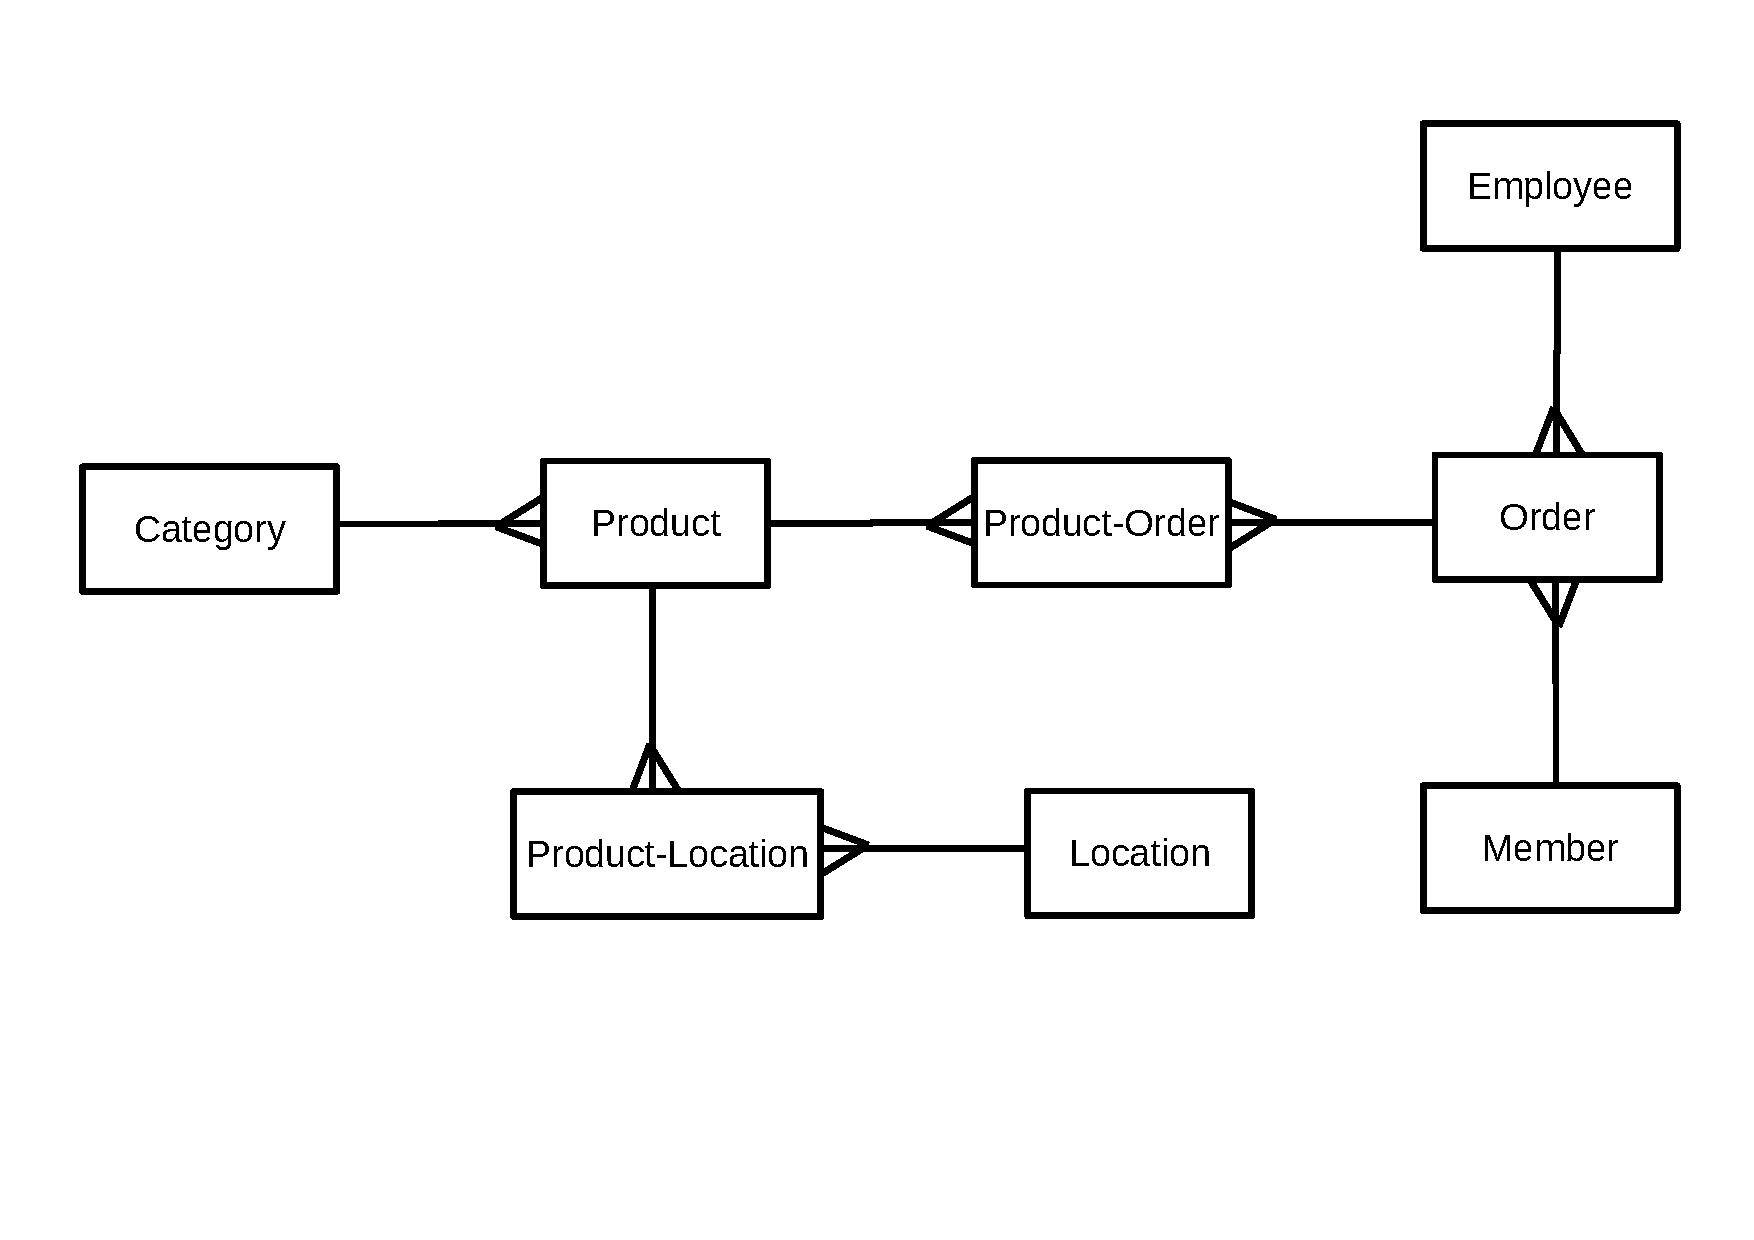
\includegraphics[width=14cm]{ERDiagramDesign.pdf}\hspace*{\fill}
\end{figure}

\subsubsection{Entity Descriptions}

Product(\textbf{ProductID}.Product Name, Size, Price, Stock)

Order(\textbf{OrderID},\textit{MemberID, EmployeeID}, Date, Time)

ProductOrder(\textit{ProductID, OrderID}, Quantity)

Location(\textbf{LocationID}, LocationName)

ProductLocation(\textbf{ProductID},\textit{LocationID})

Category(\textbf{Category})

Employee(\textbf{EmployeeID}, Employee First Name, Employee Last Name, Password, Employee Email)

Member(\textbf{MemberID}, Title, First Name, Last Name, HouseNo., Street, town, City, County, Postcode, TelephoneNo. , Member Email)

\pagebreak

\subsubsection{1NF to 3NF}



\begin{center}
    \begin{tabular}{|p{4cm}|}
        \hline
        \textbf{Un-normalised (UNF)}\\ \hline
	{ProductID}\\ \hline
	{OrderID}\\ \hline
	{ProductName}\\ \hline
	{Size}\\ \hline
	{Catagory}\\ \hline
	{Price}\\ \hline
	{LocationID}\\ \hline
	{Location Name}\\ \hline
	{Stock}\\ \hline
	{Quantity}\\ \hline
	{Date}\\ \hline
	{Time}\\ \hline
	{MemberID}\\ \hline
	{Title}\\ \hline
	{First Name}\\ \hline
	{Last Name}\\ \hline
	{House / Flat No.}\\ \hline
	{Street}\\ \hline
	{Town}\\ \hline
	{City}\\ \hline
	{County}\\ \hline
	{Postcode}\\ \hline
	{Telephone Number}\\ \hline
	{Memebr Email}\\ \hline
	{Employee ID}\\ \hline
	{Employee FirstName}\\ \hline
	{Employee LastName}\\ \hline
	{Employee Password}\\ \hline
	{Employee Email}\\ \hline
   \end{tabular}
\end{center}	
	
	

\begin{center}
    \begin{tabular}{|p{4cm}|p{4cm}|}
        \hline
	 \multicolumn{2}{|c|}{1NF} \\ \hline
	\textbf{Repeating} & \textbf{ Non Repeating}\\ \hline
	\textbf{ProductID}  & \textbf{OrderID}\\ \hline
	\textbf{OrderID} & {Date}\\ \hline
	{Product Name} & {Time}\\ \hline
	{Size} & {MemberID}\\ \hline
	{Category} & {Title}\\ \hline
	{Price} & {Member First Name}\\ \hline
	{LocationID} & {Member Last Name}\\ \hline
	{LocationName} & {House / Flat No.}\\ \hline
	{Stock} & {Street}\\ \hline
	{Quantity} & {Town}\\ \hline
	{} & {City}\\ \hline
	{} & {County}\\ \hline
	{} & {Postcode}\\ \hline
	{} & {Telephone No.}\\ \hline
	{} & {Member Email}\\ \hline
	{} & {Employee ID}\\ \hline
	{} & {Employee First Name}\\ \hline
	{} & {Employee Last Name}\\ \hline
	{} & {Password}\\ \hline
	{} & {Employee Email}\\ \hline
   \end{tabular}
\end{center}

\pagebreak

\begin{center}
    \begin{tabular}{|p{4cm}|p{4cm}|p{4cm}|}
        \hline
	 \multicolumn{3}{|c|}{2NF} \\ \hline
	\textbf{ProductID}  & \textbf{OrderID} & \textbf{ProductID}\\ \hline
	\textbf{OrderID} & {Date} & {Product Name} \\ \hline
	{Quantity} & {Time} & {Size} \\ \hline
	{} & {MemberID} & {Category} \\ \hline
	{} & {Title} & {Price} \\ \hline
	{} & {First Name} & {Stock} \\ \hline
	{} & {Last Name} & {LocationID} \\ \hline
	{} & {House / Flat No.} & {Location Name} \\ \hline
	{} & {Street} & {Stock} \\ \hline
	{} & {Town} & {} \\ \hline
	{} & {City} & {} \\ \hline
	{} & {County} & {} \\ \hline
	{} & {Postcode} & {} \\ \hline
	{} & {Telephone Number} & {} \\ \hline
	{} & {Member Email} & {} \\ \hline
	{} & {EmployeeID} & {} \\ \hline
	{} & {Employee First Name} & {} \\ \hline
	{} & {Employee Last Name} & {} \\ \hline
	{} & {Password} & {} \\ \hline
	{} & {Employee Email} & {} \\ \hline	
    \end{tabular}
\end{center}

\begin{flushleft}
\begin{center}
    \begin{tabular}{|p{3cm}|p{3cm}|p{3cm}|p{2cm}|}
        \hline
	 \multicolumn{4}{|c|}{3NF} \\ \hline
	\textbf{Product ID}  & \textbf{Product-Order ID} & \textbf{Order ID} & \textbf{Employee ID} \\ \hline
	{Product Name} & \textit{ProductID} & \textit{Member ID} & {Employee First Name} \\ \hline
	{Size} & \textit{Order ID} & \textit{Employee ID} & {Employee Last Name} \\ \hline
	{Price} & {Quantity} & {Date} & {Password} \\ \hline
	{Stock} & {} & {Time} & {Employee Email} \\ \hline
	{} & {} & {} & {}\\ \hline
	{} & {} & {} & {}\\ \hline
	\textbf{Member ID} & \textbf{Product ID} & \textbf{Location ID} & \textbf{Category}\\ \hline
	{Title} & \textit{Location ID} & {Location Name} & {}\\ \hline
	{First Name} & {} & {} & {}\\ \hline
	{Last Name} & {} & {} & {}\\ \hline
	{House / Flat No.} & {} & {} & {}\\ \hline
	{Street} & {} & {} & {}\\ \hline
	{Town} & {} & {} & {}\\ \hline
	{City} & {} & {} & {}\\ \hline
	{County} & {} & {} & {}\\ \hline
	{Postcode} & {} & {} & {}\\ \hline
	{Telephone Number} & {} & {} & {}\\ \hline
	{Memebr Email} & {} & {} & {}\\ \hline
    \end{tabular}
\end{center}
\end{flushleft}

\subsection{SQL Queries}

I have used python to format the following SQL Statements:
\begin{python}
"""create ProductTable(
 ProductID INTEGER,
 ProductName TEXT,
 Category TEXT,
 Price INTEGER,
 PRIMARY KEY(ProductID))
\end{python}

This is the SQL Statement for creating a new product table. The attributes ProductName, Category and Price are entered by the user, and the ProductID is assigned to the product automatically. The next SQl statement then adds a product to the table.
\begin{python}
"""insert into
Product(ProductName,Category,Price,Stock) values (product_name, category, price, stock)
\end{python}

the attributes product name, category, price and stock are entered by the user and passed into the product table created in the previous SQL statement. One the table has multiple products in it, finding products quickly may become an issue. The next SQL statement allows the user to search for a specific product.
\begin{python}
        	"""select *
        	 from Product
        	 where ProductName = ProductNameSearch
\end{python}

Once the user has found the product they want there are many different things the user can do with the data. If the user notices inaccuracy in the product data they can edit ti using the following SQL statement.
\begin{python}
	"""update Product set
	ProductName = NewProductName
	 Category = NewCategory
 	Price = NewPrice
 	where ProductID = ProductIDSearch
\end{python}
If the user decides they want to remove the product entirely instead of editing the data they can use the following SQL statement. The user enters the ProductID of the Product in which they would like to remove form the table, The ProductID is assigned to the variable `ProductIDToDelete' This is then passed into the SQL statement and the product is deleted form the table and database.
\begin{python}
	"""delete from Product
 where ProductID = ProductIDToDelete
\end{python}
If the user does not know the specific name of the product but they know what category the product comes under, the following SQL Statement allows the user to enter a category, and all the products that fall under that category are displayed in the table.
\begin{python}
	"""select ProductName, Category
	from Product
	where Category = EnterCategory
\end{python}

\section{Security and Integrity of the System and Data}

\subsection{Security and Integrity of Data}

My system will store personal information about the members and also the employees. Therefore, my system must follow the Data Protection Act. This means that the Database should be kept upto date, removing any data that is older than roughly 5 or 6 years old. This can be done when the system first starts up. The system can check the date in which the data was added and if the data has been in the database for over 6 years it shall be removed from the database. Before any of the data in the system can be accessed, a user must must Log in to the system with a username and password combination. This allows only authorized users to handle the data. Inaccuracies in databases can sometimes be caused by erroneous data being entered by the user. For example is the user wanted to enter the word `Password' they may accidentally enter `Password'. This sort of error can lead to data becoming inaccurate, to minimize the risk of this happening, as many drop down menus and choice buttons will be supplied as possible. I will also need to include Referral Integrity to my database. This will add checks when adding, removing and deleting data to all the fields are complete and no key data is missing.

\subsection{System Security}
To access any data on the system, a correct employee username and password must be entered. To further secure the data, employee accounts can only be added and deleted through the admin account (my clients account). None of the system will be accessable until a correct username and password combination is entered. An additional Security step, could be to ensure all employee passwords are updated every 30 days. To ensure my system follows the Data Protection Act, my system must: \par \par
\begin{itemize}
\item Must not be Transfered to Other Countries
\item Must be stored securely, to ensure that it is only accessed by authorized people
\item The data in the system should not be passed onto any other computer
\item Any data older than 6 years old should be destroyed.
\item The data should be updated regularly to ensure it is accurate.
\item Only data that is necessary should be stored.
\end{itemize}
\section{Validation}


\begin{tabular}{|p{2cm}|p{2cm}|p{3.5cm}|p{4cm}|}
        \hline
        \textbf{Data} & \textbf{Example} & \textbf{Validation / Verification} & \textbf{Comments} \\ \hline
	ProductName &  OPTEX Ear Drops & Presence check & To ensure that the Product Name is entered.\\ \hline
	Size & 750 grams & Valid Integer check \par Presence check & To enusre a Size is entered and to make sure that only an interger is entered between 1 - 1000 \\ \hline
          Price & 9.99 & Valid Integer Check \par Valid Range Check \par Presence Check & To ensure a price is entered and to ensure only integers are entered and the price entered is between £0.01 - £500.00\\ \hline
          Catagory &  Dog food &  Presence check &  To ensure a Category is entered \\ \hline
	Title &  Mrs. & Range Check \par Presence check & To ensure a Title is entered between 1 and 5 characters \\ \hline
          Member Firstname & Thomas & String Check \par Presence check & To ensure a name is entered and to ensure the name does nto contain integers or other characters.\\ \hline
          Member LastName & Brennan & String Check \par Presence check & To ensure a last name is entered and to ensure the name only contains letters.\\ \hline
          House No. &  66 & Range Check \par Integer check \par Presence Check & To ensure a Hosue Number is entered and to ensure its an integer between 1-500\\ \hline
	Street &  Market Street & Presence Check & to ensure a street is entered\\ \hline
	Town &  Fordham & Presence Check & to ensure a town is entered\\ \hline
         City &  Ely & Presence Check & to ensure a city is entered\\ \hline
         County & Cambridge & Presence Check & to ensure a county is entered\\ \hline
         Postcode & CB7 5DJ & Postcode Check \par Presence Check \par Format Check & To ensure a postcode is entered, to ensure it is in the correct format. A Validation table for postcodes is specified below. \\ \hline
\end{tabular}

\begin{tabular}{|p{2cm}|p{2cm}|p{3.5cm}|p{4cm}|}
        \hline
         Telephone No. & 07764563958 & Presence Check \par Length Check \par Integer Check & To ensure a phone number is entered, that the phone number only contains intergers and is exactly 11 characters long. \\ \hline
	Member Email & 31477@ longroad.ac.uk & Presence check \par Format Check & There must be an email present and it must contain the `@' symbol.\\ \hline
	Employee First Name & Matthew & Presence check \par Integer Check & The user must enter a name and it must not contain integers \\ \hline
	Employee Last Name &  Ling & Presence check \par Integer Check & The user must enter a name and it must not contain integers \\ \hline
	Employee Password & Password123 & Presence Check \par Length Check & a password must be entered but it may be no longer than 18 characters. \\ \hline
	Employee Email &  example@ email.com & Presence check \par Format Check & There must be an email present and it must contain the `@' symbol. \\ \hline
	Date &  7/11/2014 & Presence check \par Format check \par Range check & a date must be entered it must be in the format DD/MM/YYYY, and the Days must be in range 1-31, month must be in rang 1-12 and year must be in range 2014 - 2114\\ \hline
	Time &  22:11 & Presence Check \par Format Check \par Range check & A time must be entered, it must be in the format HH:MM where the hour must be a two digit number in range 00-24 and the minutes must be a two digit number in range 00-59\\ \hline
	Location Name & Storage Room & Presence Check \par Integer Check & A name must be entered but must not containa any integegers \\ \hline
  \end{tabular}

\pagebreak


\begin{figure}[H]
\caption{Postcode Validation table} \label{fig: Postcode Validation table}
\begin{tabular}{|p{2cm}|p{3cm}|p{2cm}|}
        \hline
        \textbf{Format} & \textbf{Coverage} & \textbf{Example} \\ \hline
        \textbf{AA9A 9AA} & EC1-EC4, NW1W, SE1P, SW1 & EC1A 1BB \\ \hline
        \textbf{A9A 9AA} & E1W, N1C, N1P & W1A 0AX \\ \hline
        \textbf{A9 9AA} & B, E, G, L, M, N, S, W & M1 1AE \\ \hline
         \textbf{A99 9AA} & B, E, G, L, M, N, S, W & B33 8TH \\ \hline
         \textbf{AA9 9AA} & All Other Postcodes & CB7 5LQ \\ \hline
         \textbf{AA99 9AA} & All Other Postcodes & DN55 1PT \\ \hline
  \end{tabular}
\par
\par
  The format is as follows, where \textbf{A} signifies a letter and \textbf{9} signifies a digit.
\end{figure}



\section{Testing}
\begin{landscape}

\subsection{Outline Plan}
\begin{center}
    \begin{tabular}{|p{2cm}|p{5cm}|p{5cm}|p{4cm}|}
        \hline
        \textbf{Test Series} & \textbf{Purpose of Test Series} & \textbf{Testing Strategy} & \textbf{Strategy Rationale}\\ \hline
	1. & Test the flow of control between the user interfaces & Top Down Testing &  \\ \hline
	2. & Test validation of data inputs & Bottom Up testing Testing &  Each input and output will be tested when they're developed\\ \hline
	3. & Test Data is stored in the correct location & Black-Box Testing & \\ \hline
	4. & Test algorithms and SQL statements to ensure the output is correct & Black box testing &\\ \hline
	5. & Test the system fulfills the specification & Acceptance testing & \\ \hline

    \end{tabular}
\end{center}

\subsection{Detailed Plan}
\pagebreak

\begin{flushleft}
    \begin{longtable}{|p{1.5cm}|p{2.5cm}|p{2.5cm}|p{2cm}|p{2cm}|p{2cm}|p{2cm}|p{2cm}|}
        \hline
        \textbf{Test Series} & \textbf{Purpose of Test} & \textbf{Test Description} & \textbf{Test Data} & \textbf{Test Data Type (Normal/ Erroneous/ Boundary)} & \textbf{Expected Result} & \textbf{Actual Result} & \textbf{Evidence}\\ \hline
	1.01 & Test the Arrow button to see if it works successfully & The Arrow Button Should change to the Product Search Interface if log in details are correct & Click the arrow button & Normal & The Product Search Interface should be displayed &&  \\ \hline
	1.02 & Test the keyboard shortcut assigned to the arrow button works successfully & The Keyboard Shortcut Should change to the Product Search Interface if log in details are correct & Press the Keyboard Shortcut after legitimate log in details are entered &  Normal &The Product Search Interface should be displayed &&  \\ \hline
	1.03 & Test the Reset Password Here Link & When clicked the Link should change to the reset password interface & Left mouse click on the Reset Password Link &  Normal & The Reset Password Interface should be displayed &&  \\ \hline
	1.04 & Test the Log Off button to see if it works successfully & Left mouse clicking the log off button should return back to the log in interface & Left mouse click Log off button &  Normal & The Log in interface should be displayed && \\ \hline
	1.05 & Test to see if the Add new product option works successfully & The user should left click on the product tab then left click on the Add new product Option. & Left click Add new product button &  Normal &  The interface should change to the Add new product interface&& \\ \hline
	1.06 & Test to see if the Delete Product button works & Clicking on the product tab then clicking on the delete product option & Left mouse click Delete a product button &  Normal & Interface should change to Delete a product interface&& \\ \hline
	1.07 & Test to see if the manage stock button works successfully & Clicking on the Manage Stock button to see what the outcome is & The Manage Product button, under the Stock tab should be left clicked &  Normal & The Stock Management interface should be displayed. && \\ \hline
	1.08 & Test to see if the Product restock button works & Clicking the Product restock button to see the result & left clicking the Stock tab then left clicking the Product restock tab &  Normal & The Stock management interface should be displayed. && \\ \hline
	1.09 & Test to see if the add a new member button works & The Add new member button should change to the Add new memebr interface & Left clicking the add new member button under the member tab &  Normal & the Add new member interface should be displayed&& \\ \hline
	1.10 & Testing to see what happens when remove member is clicked & left clicking the delete member button and recording outcome & Left clicking remove a member under the member tab & Normal & the Remove a member interface should be displayed && \\ \hline
	1.11 & Test to see if the add a new employee button works & The Add new employee button should change to the Add new employee interface & Left clicking the add new employee button under the employee tab &  Normal & the Add new employee interface should be displayed&& \\ \hline
	1.12 & Testing to see what happens when remove employee is clicked & left clicking the employee member button and recording outcome & Left clicking remove a employee under the employee tab & Normal & the Remove a employee interface should be displayed && \\ \hline
	2.01 & Testing valid characters and range of Product Name & entering a range of different characters to see which ones are valid & Test123@+ & Normal & The string Test should be accepted however, the characters `123' and `@+' should not be accepted as they are integers and special characters && \\ \hline
	2.02 & testing to see which file types are valid for Product Image & entering a range of file types to see which are valid & test.jpg, test.bnp, test.txt, test.png, test.gif, test.doc, test.pdf & Normal & The only accepted file types should be .jpg and .png. No other file extensions should be valid. && \\ \hline
	2.03 & Testing to see which characters are valid in Price & entering a range of characters into price to see which are accepted & test123@+ & Normal & Only 123 should be accepted because  a price cannot contain letters or special characters && \\ \hline
	2.04 & Testing to see which characters are valid in Stock & entering a range of characters into the stock field and seeing which are valid & test123@+ & Normal & The letters `test' and special characters `@+' should be invalid because as the stock is only defined by integers.&& \\ \hline
	2.05 & Testing to see which characters are valid in Name & Entering a range of characters into name and seeing which ones are valid & Test123@+ & Normal & Only the letters `test' should be valid as a name cannot contain integers or special characters.&& \\ \hline
	2.06 & seeing which characters are valid in email & seeing if a valid email is required to enter into this field & Bob.com, Bob@email, Bob@email.com & Normal & Only Bob@Email.com should be accepted. No string should be accepted unless it contains the `@' symbol followed by at least one `.' && \\ \hline
	2.07 & testing for validation in telephone number & entering different numbers into the field to see which are valid & 999, 01234567890, 012345678987654 & Normal & Only 01234567890 should be valid as `999' is too short and 012345678987654 is too long. && \\ \hline
	3.01 & Ensuring all product data is stored in the product table & Entering a product then ensuring all of its data is input into the Product table & Normal & Product: Dog Food & The ProductName should be Dog Food and the rest of the data should be stored in the Product Table && \\ \hline
	3.02 & Ensuring all member data is stored in the member table & Entering a member then ensuring all of its data is input into the member table & Normal & Member: Bruce Wayne & The MemberName should be Bruce Wayne  and the rest of the data should be stored in the Member Table && \\ \hline
	3.03 & Ensuring all Employee data is stored in the Employee table & Entering a employee then ensuring all of its data is input into the Employee table & Normal & Employee: Clark Kent & The EmployeeName should be Clark Kent and the rest of the data should be stored in the Employee Table && \\ \hline
	4.01 & Ensuring the product table is created properly & Creating the product table and adding a product to ensure its working properly & adding product: Dog Food & normal & The Table should be created and the product Dog Food should be added successfully. Al the data should be in its corresponding column && \\ \hline
	4.02 & Deleting a product from the database &  Entering a ProductID to delete then seeing if it was deleted successfully & ProductID = 2 & normal & The product database should be viewed, then a productID from a Product should be taken from the database should. this ProductID should be entered into the SQL statement. If the statement worked, the product should no longer be in the database && \\ \hline

    \end{longtable}
\end{flushleft}
\end{landscape}